% -*- mode: LaTeX; TeX-PDF-mode: t; -*-
% Add the listed directories to the search path
% (allows easy moving of files around later)
% these paths are searched AFTER local config kpsewhich

% *.sty, *.cls
\makeatletter
\def\input@path{{@resources/texlive/texmf-local/tex/latex//}
        ,{@resources/texlive/latex//}
        ,{@local//}
        }
\makeatother
\makeatletter
\def\bibinput@path{{@resources/texlive/texmf-local/tex/latex//}
        ,{@resources/texlive/latex//},
        ,{@local//}
        }
\makeatother
  % allow latex to find custom stuff
% LaTeX path to the root directory of the current project, from the directory in which this file resides
% and path to econtexPaths which defines the rest of the paths like \FigDir
\providecommand{\econtexRoot}{}\renewcommand{\econtexRoot}{.}
\providecommand{\econtexPaths}{}\renewcommand{\econtexPaths}{\econtexRoot/Resources/econtexPaths}
% The \commands below are required to allow sharing of the same base code via Github between TeXLive on a local machine and Overleaf (which is a proxy for "a standard distribution of LaTeX").  This is an ugly solution to the requirement that custom LaTeX packages be accessible, and that Overleaf prohibits symbolic links

\providecommand{\econtex}{\econtexRoot/Resources/texmf-local/tex/latex/econtex}
\providecommand{\pdfsuppressruntime}{\econtexRoot/Resources/texmf-local/tex/latex/pdfsuppressruntime}
\providecommand{\econark}{/Volumes/Sync/GitHub/llorracc/SolvingMicroDSOPs/SolvingMicroDSOPs-Latest/.resources/texmf-local/tex/latex/local-econark}
\providecommand{\econtexSetup}{\econtexRoot/Resources/texmf-local/tex/latex/econtexSetup}
\providecommand{\econtexShortcuts}{\econtexRoot/Resources/texmf-local/tex/latex/econtexShortcuts}
\providecommand{\econtexBibMake}{\econtexRoot/Resources/texmf-local/tex/latex/econtexBibMake}
\providecommand{\econtexBibStyle}{\econtexRoot/Resources/texmf-local/bibtex/bst/econtex}
\providecommand{\econtexBib}{economics}
\providecommand{\economics}{\econtexRoot/Resources/texmf-local/bibtex/bib/economics}
\providecommand{\notes}{\econtexRoot/Resources/texmf-local/tex/latex/handout}
\providecommand{\handoutSetup}{\econtexRoot/Resources/texmf-local/tex/latex/handoutSetup}
\providecommand{\handoutShortcuts}{\econtexRoot/Resources/texmf-local/tex/latex/handoutShortcuts}
\providecommand{\handoutBibMake}{\econtexRoot/Resources/texmf-local/tex/latex/handoutBibMake}
\providecommand{\handoutBibStyle}{\econtexRoot/Resources/texmf-local/bibtex/bst/handout}

\providecommand{\FigDir}{\econtexRoot/Figures}
\providecommand{\CodeDir}{\econtexRoot/Code}
\providecommand{\DataDir}{\econtexRoot/Data}
\providecommand{\SlideDir}{\econtexRoot/Slides}
\providecommand{\TableDir}{\econtexRoot/Tables}
\providecommand{\ApndxDir}{\econtexRoot/Appendices}

\providecommand{\ResourcesDir}{\econtexRoot/Resources}
\providecommand{\rootFromOut}{..} % APFach back to root directory from output-directory
\providecommand{\LaTeXGenerated}{\econtexRoot/LaTeX} % Put generated files in subdirectory
\providecommand{\econtexPaths}{\econtexRoot/Resources/econtexPaths}
\providecommand{\LaTeXInputs}{\econtexRoot/Resources/LaTeXInputs}
\providecommand{\LtxDir}{}
\providecommand{\EqDir}{Equations} % Put generated files in subdirectory


\documentclass[BufferStockTheory]{subfiles}
   

% LaTeX path to the root directory of the current project, from the directory in which this file resides
% and path to econtexPaths which defines the rest of the paths like \FigDir
\providecommand{\econtexRoot}{}\renewcommand{\econtexRoot}{.}
\providecommand{\econtexPaths}{}\renewcommand{\econtexPaths}{\econtexRoot/Resources/econtexPaths}
% The \commands below are required to allow sharing of the same base code via Github between TeXLive on a local machine and Overleaf (which is a proxy for "a standard distribution of LaTeX").  This is an ugly solution to the requirement that custom LaTeX packages be accessible, and that Overleaf prohibits symbolic links

\providecommand{\econtex}{\econtexRoot/Resources/texmf-local/tex/latex/econtex}
\providecommand{\pdfsuppressruntime}{\econtexRoot/Resources/texmf-local/tex/latex/pdfsuppressruntime}
\providecommand{\econark}{/Volumes/Sync/GitHub/llorracc/SolvingMicroDSOPs/SolvingMicroDSOPs-Latest/.resources/texmf-local/tex/latex/local-econark}
\providecommand{\econtexSetup}{\econtexRoot/Resources/texmf-local/tex/latex/econtexSetup}
\providecommand{\econtexShortcuts}{\econtexRoot/Resources/texmf-local/tex/latex/econtexShortcuts}
\providecommand{\econtexBibMake}{\econtexRoot/Resources/texmf-local/tex/latex/econtexBibMake}
\providecommand{\econtexBibStyle}{\econtexRoot/Resources/texmf-local/bibtex/bst/econtex}
\providecommand{\econtexBib}{economics}
\providecommand{\economics}{\econtexRoot/Resources/texmf-local/bibtex/bib/economics}
\providecommand{\notes}{\econtexRoot/Resources/texmf-local/tex/latex/handout}
\providecommand{\handoutSetup}{\econtexRoot/Resources/texmf-local/tex/latex/handoutSetup}
\providecommand{\handoutShortcuts}{\econtexRoot/Resources/texmf-local/tex/latex/handoutShortcuts}
\providecommand{\handoutBibMake}{\econtexRoot/Resources/texmf-local/tex/latex/handoutBibMake}
\providecommand{\handoutBibStyle}{\econtexRoot/Resources/texmf-local/bibtex/bst/handout}

\providecommand{\FigDir}{\econtexRoot/Figures}
\providecommand{\CodeDir}{\econtexRoot/Code}
\providecommand{\DataDir}{\econtexRoot/Data}
\providecommand{\SlideDir}{\econtexRoot/Slides}
\providecommand{\TableDir}{\econtexRoot/Tables}
\providecommand{\ApndxDir}{\econtexRoot/Appendices}

\providecommand{\ResourcesDir}{\econtexRoot/Resources}
\providecommand{\rootFromOut}{..} % APFach back to root directory from output-directory
\providecommand{\LaTeXGenerated}{\econtexRoot/LaTeX} % Put generated files in subdirectory
\providecommand{\econtexPaths}{\econtexRoot/Resources/econtexPaths}
\providecommand{\LaTeXInputs}{\econtexRoot/Resources/LaTeXInputs}
\providecommand{\LtxDir}{}
\providecommand{\EqDir}{Equations} % Put generated files in subdirectory



% \usepackage{econark-ifsubfile} is in main preamble
% where it sets macros indicating that the doc being
% compiled is NOT a subfile.
% \usepackage{econark-ifsubfile} in the subfile preamble
% is NOT EXECUTED when the content is read in by main
% so this correctly defines what is needed
\usepackage{econark-ifsubfile}

% Get xrefs -- esp to apndx -- from main file; only works if main file has already been compiled
\xrsetup{BufferStockTheory}
\externaldocument{BufferStockTheory}
  
\begin{document}

\hypertarget{The-Problem}{}
\section{Theoretical Foundations}\label{sec:Theory}

This section formalizes the consumer income fluctuation problem and proves the existence of a limiting non-degenerate solution. In doing so, we also introduce our consumer patience conditions and use them to derive the consumer's MPCs. The MPCs are formulae, for any period $t$ earlier than the terminal period $T$, for the maximum and minimum MPCs as wealth approaches zero and infinity.  If the environment is that of an infinite-horizon `income fluctuation problem,' our formulae yield the limiting upper and lower bounds of the limiting non-degenerate solution.


We first state the finite horizon problem and then define the limiting solution as the limit of finite horizon solutions as the terminal period becomes arbitrarily distant. This way, the economic intuition of limiting consumer behaviour can be directly linked to consumer behaviour in life-cycle models (see \cite{gpLifeCycle} for an instance where buffer stock saving is discussed in the context of a life-cycle model). Nonetheless for the class of problems we consider, a non-degenerate limiting solution, if it exists, is mathematically equivalent (\cite{bertsekas2012dynamic}, Ch. 1.) to a stationary solution to an infinite stochastic sequence problem commonly used in the literature (for example, \cite{mstIncFluct}). 

\label{sec:Foundations}
\subsection{Setup}\label{subsec:Setup}

We start by stating the consumer problem with permanent income growth in levels and then normalize by permanent income. The normalized problem then becomes the subject of our formal results in the paper. 

Our time index $t$ can take on values in $\{T,T-1,T-2,\dots \}$. We assume that our consumer has a Constant Relative Risk Aversion (CRRA) per-period utility function, $\uFunc(c)=\frac{c^{1-\CRRA}}{1-\CRRA}$, where $\CRRA>1$. The term $\DiscFac$ is the (strictly positive) discount factor. In each period $t$, the consumer faces independently and identically distributed (iid) income shocks, with the permanent shock given by $\permShk_{t} \in \Reals_{++}$ and the transitory shock by $\tranShkAll_{t} \in \Reals_{+}$.\footnote{Formally, we assume $\left\{\permShk_{t},\tranShkAll_{t}\right\}_{t=-\infty}^{T}$ is a sequence of iid random variables defined on a common probability space $(\Omega, \Sigma, \mathbb{P})$. When used without the time subscript, $\permShk$ and $\tranShkAll$ are the canonical random variables with distributions $\mathbb{P}\circ \permShk_{0}^{-1}$ and $\mathbb{P}\circ \tranShkAll_{0}^{-1}$, respectively.}

In each $t$, the finite horizon value function for the problem in levels will be denoted by $\vFuncLvl_{t}$, with $\vFuncLvl_{t}\colon \Reals_{++}^{2}\rightarrow \Reals$. Value, $\vFunc_{t}(\mLvl_{t}, \permLvl_{t})$, depends on two strictly positive state variables: `market resources' $\mLvl_{t}$ and permanent income $\permLvl_{t}$.
After the terminal period, we assume the consumer cannot die in debt:
%
\begin{equation}\label{eq:NoDebtAtDeath}
\cLvl_{T} \leq  \mLvl_{T} .
\end{equation}
%
Letting $\vFuncLvl_{T+1} = 0$, it follows that the value function for the terminal period satisfies $\vFuncLvl_{T} = \uFunc(\mNrm_{T})$.
For $t<T$, the finite-horizon value functions are recursively defined by:

%
\begin{verbatimwrite}{Equations/supfn}
  \begin{align}\label{eq:levelRecProblem}
    \vFuncLvl_{t}(\mLvl_{t}, \permLvl_{t})\colon & = \max_{0 < \cLvl_{t} \leq \mLvl_{t}} \uFunc(\cLvl_{t}) + \DiscFac \Ex_{t}\vFuncLvl_{t+1}(\mLvl_{t+1}, \permLvl_{t+1}), \qquad (\mLvl_{t}, \permLvl_{t})\in \Reals_{++}^{2} \tag{$\mathscr{P}_{L}$}
  \end{align}
\end{verbatimwrite}
  \begin{align}\label{eq:levelRecProblem}
    \vFuncLvl_{t}(\mLvl_{t}, \permLvl_{t}) & = \max_{0 \leq\cLvl_{t} \leq \mLvl_{t}} \uFunc(\cLvl_{t}) + \DiscFac \Ex_{t}\vFuncLvl_{t+1}(\mLvl_{t+1}, \permLvl_{t+1}) \tag{$\mathscr{P}_{L}$}
  \end{align}

\noindent where i) $\cLvl_{t}$ is the level of consumption at time $t$, ii) $\Ex_{t}$ is the expectation operator over the shocks $\permShk_{t+1}$ and $\tranShkAll_{t+1}$\hypertarget{checkRestrictions}{}\hypertarget{DBCparts}{}, and iii) $\mLvl_{t+1}$ is determined from this period's $\mLvl_{t}$ and choice of $\cLvl_{t}$ as follows:\footnote{For maximal clarity, we have separately described every step in the dynamic budget evolution.
The steps are broken down also so that the notation of the paper will correspond exactly to the variable names in the \href{https://github.com/econ-ark/HARK} toolkit, because it is required for solving life cycle problems.}%$^{,}$\footnote{Allowing a stochastic interest factor would complicate the notation but not affect the points we want to address; however, see~\cite{benhabibWealth},~\cite{maTodaRich}, and~\cite{mstIncFluct} for the implications of capital income risk for the distribution of wealth and other interesting questions not considered here.}
%
\begin{verbatimwrite}{Equations/DBCparts}
  \begin{equation}\label{eq:DBCparts} % Don't define it if already defined
    \begin{split}
      \aLvl_{t}     & = \mLvl_{t}-\cLvl_{t}  \\
      \kLvl_{t+1}   & = \aLvl_{t} \notag \\
      \permLvl_{t+1}  & = \permLvl_{t} \underbrace{\PermGroFac\permShk_{t+1}}_{:= \Rnd{\PermGroFac}_{t+1}} \notag \\
      \mLvl_{t+1}  & =   \underbrace{\Rfree \kLvl_{t+1}}_{:= \bLvl_{t+1}}  +\underbrace{\permLvl_{t+1}\tranShkAll_{t+1}}_{:= \yLvl_{t+1}}. \notag
    \end{split}
  \end{equation}
\end{verbatimwrite}
  \begin{equation}\label{eq:DBCparts} % Don't define it if already defined
    \begin{split}
      \aLvl_{t}     & = \mLvl_{t}-\cLvl_{t}  \\
      \kLvl_{t+1}   & = \aLvl_{t} \notag \\
      \permLvl_{t+1}  & = \permLvl_{t} \underbrace{\PermGroFac\permShk_{t+1}}_{:= \Rnd{\PermGroFac}_{t+1}} \notag \\
      \mLvl_{t+1}  & =   \underbrace{\Rfree \kLvl_{t+1}}_{:= \bLvl_{t+1}}  +\underbrace{\permLvl_{t+1}\tranShkAll_{t+1}}_{:= \yLvl_{t+1}}. \notag
    \end{split}
  \end{equation}

%
The consumer's assets at the end of $t$, $\aLvl_{t}$, translate one-for-one into capital $\kLvl_{t+1}$ at the beginning of the next period.
In turn, $\kLvl_{t+1}$ is augmented by a fixed interest factor $\Rfree$ to become the consumer's financial (`bank') balances $\bLvl_{t+1} = \Rfree \kLvl_{t+1}$.`Market resources,' $\mLvl_{t+1}$,  are the sum of financial wealth $\Rfree \kLvl_{t+1}$ and noncapital income $\yLvl_{t+1}=\permLvl_{t+1}\tranShkAll_{t+1}$ (permanent noncapital income $\permLvl_{t+1}$ multiplied by the transitory shock $\tranShkAll_{t+1}$).
Permanent noncapital income $\permLvl_{t+1}$ is derived from $\permLvl_{t}$ by application of a growth factor $\PermGroFac$,\footnote{A time-varying $\PermGroFac$ has straightforward consequences for the analysis below; this is an option allowed for in the \href{https://econ-ark.org}{HARK} toolkit.} modified by the permanent income shock $\permShk_{t+1}$, and the resulting idiosyncratic growth factor for permanent income is written as $\Rnd{\PermGroFac}_{t+1}$.

Letting $n$ denote the planning horizon, the finite-horizon problems furnish a sequence of value functions $\{\vFuncLvl_{T},\vFuncLvl_{T-1},\ldots,\vFuncLvl_{T-n}\}$ and associated consumption functions $\{\cFuncLvl_{T},\cFuncLvl_{T-1},\ldots,\cFuncLvl_{T-n}\}$.
The limiting consumption function, denoted by $\usual{\cFuncLvl}(\mLvl,\permLvl) = \lim\limits_{n \rightarrow \infty} \cFuncLvl_{T-n}(\mLvl,\permLvl)$, will be called a `non-degenerate limiting solution' if  neither $\usual{\cFuncLvl}=0$ everywhere (for all $(\mLvl,\permLvl)$) nor $\usual{\cFuncLvl}=\infty$ everywhere.

Before turning to the normalized problem, we present the income process and its implications for the consumer problem.
The following assumption defines the income process.

\begin{assumI}\label{ass:shocks}(Friedman-Muth Income Process).
For each $t$:
\begin{enumerate}
\item The permanent shock, $\permShk_{t}$, satisfies $\Ex[{\permShk}_{t}]=1$ and  $\permShk_{t}\in [\permShkIndMin,\permShkIndMax]$ s.t. $0 < \permShkIndMin \leq 1$ and $1 \leq \permShkIndMax < \infty$. 
\item The transitory shock, $\tranShkAll_{t}$, satisfies: 
\begin{verbatimwrite}{Equations/TranShkDef}
  \begin{equation}
    \tranShkAll_{t}=
    \begin{cases}
      0\phantom{_{t+1}/\pNotZero} & \text{with probability $\pZero > 0$} \\
      \tranShkEmp_{t}/\pNotZero      & \text{with probability $\pNotZero  $}, % \equiv 1-\pZero
    \end{cases} \label{eq:TranShkDef}
  \end{equation}
\end{verbatimwrite}
  \begin{equation}
    \tranShkAll_{t}=
    \begin{cases}
      0\phantom{_{t+1}/\pNotZero} & \text{with probability $\pZero > 0$} \\
      \tranShkEmp_{t}/\pNotZero      & \text{with probability $\pNotZero  $} % \equiv 1-\pZero
    \end{cases} \label{eq:TranShkDef}
  \end{equation}

\noindent for iid random variable $\tranShkEmp_{t}$,  with $\Ex[{\tranShkEmp}_{t}]=1$ and $ \tranShkEmp_{t} \in [\Min{\tranShkEmp}, \bar{\tranShkEmp}]$ s.t.
$\tranShkEmpMin >0$ and $\Min{\tranShkEmp} \leq 1 \leq \Max{\tranShkEmp} < \infty$.

\end{enumerate} 
\end{assumI}

Following~\cite{zeldesStochastic}, the income process incorporates a small probability $\pZero$ that income will be zero (a `zero-income event').
At date $T-1$, the (strictly positive) probability $q$ of zero income in period $T$ will prevent the consumer from spending all resources, because saving nothing would mean arriving in the following period with zero bank balances and thus facing the possibility of being required to consume 0, which would yield utility of $-\infty$.
This logic holds recursively from $T-1$ back, so  the consumer will never spend everything, giving rise to what \cite{aiyagari:ge} dubbed a `natural borrowing constraint.'\footnote{We specify zero as the lowest-possible-income event without loss of generality \citep{aiyagari:ge}.} (Thus, the upper-bound constraint on consumption in the problem \eqref{eq:levelRecProblem} will not bind.)


\hypertarget{PDV}{}

The model looks more special than it is.
In particular, a positive probability of zero-income events may seem objectionable (despite empirical support).
However, a nonzero minimum value of $\tranShkAll$ (motivated, say, by the existence of unemployment insurance) could be handled by capitalizing the present discounted value (PDV) of minimum income into current market assets,\footnote{So long as unemployment benefits are proportional to $\permLvl_{t}$; see the discussion in Section~\ref{subsubsec:ratio}.} and transforming that model back into this one.
And no key results would change if the transitory shocks were persistent but mean-reverting (instead of iid).\@ Also, the assumption of a positive point mass for the worst realization of the transitory shock is inessential, but simplifies the proofs and is a powerful aid to intuition.


\begin{comment}
Following footnotes and text were removed from the discussion above


\footnote{\cite{rabaultBorrowing} and~\cite{lsIncFluct} analyze cases where the shock processes have unbounded support.} 

and when $\permShkIndMin=\permShkIndMax=1$ the model becomes the degenerate case with no permanent shocks
\end{comment}

\hypertarget{The-Problem-Can-Be-Rewritten-in-Ratio-Form}{}
\hypertarget{The-Problem-Can-Be-Normalized-By-Permanent-Income}{}
\subsubsection{Normalized Problem}\label{subsubsec:ratio}

Let nonbold variables be the boldface counterpart normalized by $\permLvl_{t}$, allowing us to reduce the number of states from two ($\mLvl$ and $\permLvl$) to one $(\mNrm = \mLvl/\permLvl)$.
Now, in a one-time deviation from the notational convention established in the last sentence, define nonbold `normalized value' not as $\vLvl_{t}/\permLvl_{t}$ but as $\vNrm_{t} = \vLvl_{t}/\permLvl_{t}^{1-\CRRA}$, because this allows us to write nonbold $\vFunc_{t}$, with $\vFunc_{t}\colon \Reals_{++}\rightarrow \Reals$, to denote the `normalized value function':
%
%
\begin{equation}\label{eq:veqnNrmRecBellman}
  \begin{split}
    % \begin{align*}
    \vFunc_{t}(\mNrm_{t})  & = \max_{0<\cNrm_{t}< \mNrm_{t}}~  \uFunc(\cNrm_{t}) +\DiscFac \Ex_{t}[\Rnd{\PermGroFac}_{t+1}^{1-\CRRA}\vFunc_{t+1}({\mNrm}_{t+1})],\qquad  \mNrm_{t}\in \Reals_{++}\\
    & \mbox{s.t.}
    \\ {\aNrm}_{t}  & = \mNrm_{t}-c_{t}
    \\ {\kNrm}_{t+1} & = \aNrm_{t}/\Rnd{\PermGroFac}_{t+1} =  \RNrmByGRnd_{t+1}\aNrm_{t}
    \\ {\bNrm}_{t+1} & = \kNrm_{t+1} \Rfree %\Rnd{\PermGroFac}_{t+1} %= ~  \RNrmByGRnd_{t+1}\aNrm_{t} = \RNrmByGRnd_{t+1}\aNrm_{t}
    \\ \mNrm_{t+1}  & = \bNrm_{t+1} +\tranShkAll_{t+1} ,
                      %       \end{align*}
  \end{split}  \tag{$\mathscr{P}_{N}$}
\end{equation}
where $\RNrmByGRnd_{t+1}\colon = (\Rfree/\PermGroFacRnd_{t+1})$ is a `permanent-income-growth-normalized' return factor.
(Appendix \ref{sec:recoverLevels} explains how the solution to the original problem in levels can be recovered from the normalized problem.)

The time $t$ normalized consumption \textit{policy function} for the finite-horizon problem, $\cFunc_{t}$, is defined by:
%
\begin{equation}\label{eq:cfunceq1}
    \cFunc_{t}(\mNrm_{t})\colon  = \argmax_{0<\cNrm_{t}< \mNrm_{t}}~  \uFunc(\cNrm_{t}) +\DiscFac \Ex_{t}[\Rnd{\PermGroFac}_{t+1}^{1-\CRRA}\vFunc_{t+1}(\mNrm_{t+1} )].
\end{equation}
% 
The normalized problem's first order condition becomes:
\begin{align}
  c_{t}^{-\CRRA}  & = \Rfree \DiscFac \Ex_{t}[ \Rnd{\PermGroFac}_{t+1}^{-\CRRA} \cNrm_{t+1}^{-\CRRA}].  \label{eq:scaledeuler}
\end{align}

\hypertarget{sensible}{}\hypertarget{useful}{}
\hypertarget{Definition-of-a-Nondegenerate-Solution and Bellman}{}
Since our main results pertain to the normalized problem, we define the limiting non-degenerate solution to the normalized problem formally.

\begin{definition}\label{def:nondegeneracy}(Non-degenerate Limiting Solution)
\ref{eq:veqnNrmRecBellman} has a non-degenerate limiting solution if there exists $ \usual{\cFunc}$, with $\usual{\cFunc}\colon \Reals_{++}\rightarrow \Reals_{++}$, and $ \usual{\vFunc}$, with $\usual{\vFunc}\colon \Reals_{++}\rightarrow \Reals$, such that:
%
\begin{align*}
  \usual{\cFunc}(\mNrm) =  \lim_{n \rightarrow \infty} \cFunc_{T-n}(\mNrm), \quad \usual{\vFunc}(\mNrm)  =  \lim_{n \rightarrow \infty} \vFunc_{T-n}(\mNrm), \qquad \mNrm \in \Reals_{++} \notag.
\end{align*}
\end{definition}


\hypertarget{Stationary-Bellman-Operator}{}

We use $\TMap$ to denote the stationary Bellman operator for the normalized problem.
To define $\TMap$, let $\RNrmByGRnd \colon = \Rfree/\PermGroFacRnd$ and let $\TMap$ denote the mapping $\vFunc_{t+1} \mapsto \vFunc_{t}$ given by Problem \ref{eq:veqnNrmRecBellman}:
%
\begin{equation}\label{eq:maintmap}
  \TMap \vFunc_{t+1}(\mNrm) = \max_{\cNrm \in (0, \mNrm) }  \left\{
    \uFunc(c) + \DiscFac\Ex\Rnd{\PermGroFac}^{1-\CRRA}\vFunc_{t+1}(\RNrmByGRnd(m - c) + \tranShkAll)
  \right\}, \quad m \in \Reals_{++}.  
\end{equation}
%
The mapping $\mNrm\mapsto (0, \mNrm)$ defines the feasibility correspondence.
To define $\TMap$, we excluded the boundary of the feasible values that consumption can take ($0$ and $\mNrm$) to ensure the maximand above is real-valued for all feasible values of consumption.
It is straightforward to show (using the Bellman Principle of Optimality) that a finite valued solution, $\vFunc$, to the functional equation $\TMap\vFunc = \vFunc$ defines a \hyperlink{sensible}{limiting non-degenerate solution}.
However, because the feasibility correspondence does not include the boundary of feasible consumption, existing dynamic programming arguments cannot be used to show that such a solution (a fixed point to $\TMap$) exists.


\subsubsection{Dynamic Programming Challenges}\label{subsubsec:challengesDP} \hypertarget{challengesDP}{} Standard dynamic programming \citep{stachurski2022} works by showing that $\TMap$ is a well-defined contraction map on a Banach space, which would allow us to conclude that the sequence of value functions given by Problem \ref{eq:veqnNrmRecBellman} converges to a fixed point of $\TMap$, a non-degenerate solution.
At first, we must contend with the fact that both $\uFunc$ and $\vFunc$ are unbounded below.
We resolve unboundedness by constructing a weighted-norm (see below).
Setting aside unboundedness, the natural liquidity constraint introduces a more pernicious challenge related to continuity: $\TMap$ will not a be well defined self-map on a vector space of continuous functions.
In particular, we cannot assert $\TMap$ maps continuous functions to continuous functions since the feasiblility correspondence $\mNrm\mapsto (0, \mNrm)$ is not compact-valued.

\begin{remark}\label{remark:notCompact}
Since the correspondence $\mNrm\mapsto (0, \mNrm)$ is not compact valued, the conditions of Berge's Maximum Theorem (Lemma 1, \cite{Jaskiewicz2011}) fail and $\TMap \fFunc$ may not be continuous for continuous $\fFunc$.
\end{remark}

If we reintroduce the boundary points $0$ and $\mNrm$ to the feasibility correspondence, the operator $\TMap$ will be able to map upper semicontinuous functions to upper semicontinuous functions (Lemma 1, \cite{Jaskiewicz2011}).
However, $\vFunc$ must now be defined on $\Reals_{+}$ and take on values in $\mathbb{R}_{+}\cup\{-\infty\}$ and spaces of such functions will not be a vector space.
The approach taken by \cite{Ma2022} is to impose an artificial liquidity constraint, which yields a real-valued continuation value, even if $\cNrm= \mNrm$, and forces the value function to be bounded below as a function of end-of-period assets.
This allows \cite{Ma2022} to define a functional operator operator within which the feasibiltiy correspondence is the compact interval $[0, \mNrm]$.
Without an artificial constraint, no such strategy is possible.\footnote{The challenge of continuity and compactness remains unresolved in a general setting \citep{rinconZapatero2024}.
Relevant results include \cite{Feinberg2012}, who generalize the requirement of continuity of feasibility correspondences to K-Inf-Compactness of the Bellman operator, yielding a mapping from semi-continuous to semi-continuous functions.
\cite{Shanker2017a} introduces a generalization, mild-Sup-compactness, which can be verified in the weak topology generated on the infinite dimensional product space of feasible random variables controlled by the consumers.
Our approach, by contrast, has the advantage that it can be used to verify existence using more standard tools.} 


A related approach, which uses Euler operators is used by \cite{mstIncFluct}.
While \cite{mstIncFluct} also assume an artificial liquidity constraint to bound the marginal utility of consumption, it is useful to consider how the structure of our model relates to theirs  once the artificial liquidity constraint is imposed.


\begin{remark}\label{remark:stochdiscMST}
If $\pZero=0$, \eqref{eq:veqnNrmRecBellman} becomes a special case of \cite{mstIncFluct}, with $\RNrmByGRnd_{t+1}=\Rfree/\Rnd{\PermGroFac}_{t+1}$ corresponding to the stochastic rate of return on capital and $\DiscFac \Rnd{\PermGroFac}_{t+1}^{1-\CRRA}$  corresponding to the stochastic discount factor.
\end{remark}

Notwithstanding Remark \ref{remark:stochdiscMST},  there are important economic consequences relating consumer patience to buffer stock saving due to the fact that in our problem $\RNrmByGRnd_{t+1}=\Rfree/\Rnd{\PermGroFac}_{t+1}$ is tightly tied to the `normalized stochastic discount factor,' $\DiscFac \Rnd{\PermGroFac}_{t+1}^{1-\CRRA}$; these will become apparent as we proceed.


\hypertarget{GICTheorySetup}{}
\subsection{Consumer Patience Conditions}\label{subsec:GICTheorySetup}

In order to have a central reference point for them, we now collect conditions relating consumer discounting and patience to the rate of return and income growth that underpin results in the remainder of the paper.
Assumptions \ref{ass:FVAC} - \ref{ass:RIC}  (finite value of autarky, return impatience and weak return impatience) will be used to prove the existence of limiting solutions in Section \ref{subsec:limSolExists}, and Assumptions \ref{ass:GICRaw} - \ref{ass:GICMod} (growth impatience and strong growth impatience) are required for existence of alternative definitions of a stable target buffer stock in Section \ref{sec:individStability}.


We start by generalizing the standard $\DiscFac<1$ condition to our setting with permanent income growth and uncertainty.\footnote{In light of Remark \ref{remark:stochdiscMST}, \cite{mstIncFluct} Assumption 2.1 is a generalization of this discount condition, albeit in a context with artificial liquidity constraints.} The updated condition requires that the expected net discounted value of utility from consumption is finite under our definition of `autarky' -- where consumption is always equal to permanent income.
A finite value of autarky helps guarantee that as the horizon extends, discounted value remains finite along \textit{any} consumption path the consumer might choose.
(See Appendix~\ref{sec:ApndxConcaveCFunc}).



\hypertarget{FVAC}{}
\begin{assumL}\label{ass:FVAC}(Finite Value of Autarky). 
%
$0 < \DiscFac \PermGroFac^{1-\CRRA}\Ex(\permShk^{1-\CRRA}) < 1 $.
%
\end{assumL}


We now turn to consumer patience and start with `absolute (im)patience.'
We will say that an unconstrained perfect foresight consumer exhibits absolute impatience if they optimally choose to spend so much today that their consumption must decline in the future.
The growth factor for consumption implied by the Euler equation of a perfect foresight model is $\cLvl_{t+1}/\cLvl_{t} = {(\Rfree\DiscFac)}^{1/\CRRA}$,\footnote{See \eqref{eq:cGroFac} below.} which motivates our definition of an `absolute patience factor' whose centrality (to everything that is to come later) justifies assigning to it a special symbol; we have settled on the archaic letter \href{https://en.wikipedia.org/wiki/Thorn_(letter)}{`thorn'}:
\hypertarget{APFAC}{}
\begin{equation}\label{eq:APFac}
    \APFac \colon= {(\Rfree\DiscFac)}^{1/\CRRA}.
\end{equation}

We will say that (in the perfect foresight problem) `an absolutely impatient' consumer is one for whom $\APFac < 1$; that is an absolutely impatient consumer prefers to consume more today than tomorrow (and vice versa for an `absolutely patient' consumer, whose consumption will grow over time):
\hypertarget{AIC}{}
\begin{assumL} (\textit{Absolute Impatience}). \label{ass:AIC}
$\APFac  < 1$. 
\end{assumL}

A consumer who is absolutely impatient, $\APFac<1$, satisfies the standard impatience condition commonly used in the income fluctuation literature, $\DiscFac\Rfree<1$, which guarantees the existence of a stable asset distribution when there is no permanent income growth.
However, as pointed out by \cite{szeidlInvariant} and \cite{maUnboundedDP}, $\DiscFac\Rfree<1$ is not necessary for an infinite-horizon solution.

Recall now our earlier requirement that the limiting consumption function $\cFunc(\mNrm)$ in our model must be `sensible.'
We will show below that for the perfect foresight unconstrained problem this requires
\hypertarget{RIC}{}
\begin{assumL} (\textit{Return Impatience}).\label{ass:RIC}
$\RPFac  < 1$. 
\end{assumL}

Return impatience can be best understood as the tension between the income effect of capital income and the substitution effect.
As we show below in Section \ref{subsec:PFBbenchmark}, in the perfect foresight model, it is straightforward to derive the MPC out of overall (human plus nonhuman) wealth that would result in next period's wealth being identical to the current period's wealth.
The answer turns out to be an MPC (`$\MPC$') of $\MPC=(1-\APFac/\Rfree)$.
The interesting point here is that $\MPC$ depends both on our absolute patience factor $\APFac$ and on the return factor.
This is the manifestation in this context of the interaction of the income effect (higher wealth yields higher interest income if $\Rfree>1$) and the substitution effect (which we have already captured with $\APFac$).


Next, consider the weaker condition of a consumer whose \hyperlink{APFAC}{absolute patience factor} is suitably adjusted to take account of the probability of zero income is less than the market return.

%
\hypertarget{WRIC}{}
\begin{assumL} (\textit{Weak Return Impatience}). \label{ass:WRIC}
$\underbrace{\frac{(\pZero \Rfree \DiscFac)^{1/\CRRA}}{\Rfree}}_{ = \frac{\pZero^{1/\CRRA} \APFac}{\Rfree}} < 1. \phantom{\text{{\WRIC}:~~}}$
%
\end{assumL}

This condition is `weak' (relative to the plain return impatience) because the probability of the zero income events $\pZero$ is strictly less than 1.
The role of $\pZero$ in this equation is related to the fact that a consumer with zero end-of-period assets today has a probability $\pZero$ of having no income and no assets to finance consumption (and $\mNrm_{t+1}=0$ would yield negative infinite utility).
In the case with no artificial constraint, our main results below, in Section \ref{subsec:limSolExists},  show weak return impatience and finite value of autarky are sufficient to guarantee a sensible (non-degenerate) solution.

Weak return impatience cannot be relaxed further without an artificial liquidity constraint.
Even though $\pZero^{1/\CRRA} \RPFac\rightarrow 0$ as $\pZero\rightarrow 0$ the weak return impatience condition \textit{does not} approach irrelevance as the possibility of the zero income event approaches zero.
Instead, we show below in Section \ref{subsubsec:deatonIsLimit} that the limiting consumption function with a natural constraint approaches the solution to a model with an artificial constraint.
% 


Now that we have finished discussing the requirements for a non-degenerate solution, we turn to assumptions required for stability.
We speak of a consumer whose \hyperlink{APFAC}{absolute patience factor} is less than the expected growth factor for their permanent income $\PermGroFac = \Ex[\PermGroFac \permShk])$ as exhibiting `growth impatience:' 
\hypertarget{GPFacRawDefn}{}
\hypertarget{GICRaw}{}
\begin{assumS}\label{ass:GICRaw} (\textit{Growth Impatience}).
$ \GPFacRaw  < 1$.
\end{assumS}

\begin{comment}
\begin{verbatimwrite}{Equations/GICRaw}
  \begin{equation}\begin{gathered}\begin{aligned}
        \text{\GICRaw:~~}  &&  \GPFacRaw  < 1 . \phantom{/\PermGroFac}&  \phantom{\text{\GICRaw:~~}} \label{eq:GICRaw}
      \end{aligned}\end{gathered}\end{equation}
\end{verbatimwrite}
  \begin{equation}\begin{gathered}\begin{aligned}
        \text{\GICRaw:~~}  &&  \GPFacRaw  < 1. \phantom{/\PermGroFac}&  \phantom{\text{\GICRaw:~~}} \label{eq:GICRaw}
      \end{aligned}\end{gathered}\end{equation}

\end{assumS}
\end{comment}

A final useful definition is `strong growth impatience' which holds for a consumer for whom the expectation of the \textit{ratio} of the \hyperlink{APFAC}{absolute patience factor} to the growth factor of permanent income is less than one, 
\hypertarget{GICMod}{}
\begin{assumS}(\textit{Strong Growth Impatience}). \label{ass:GICMod}
$ \Ex\left[\frac{\APFac}{\PermGroFac \permShk}\right] = \GPFacMod  < 1.$
\end{assumS}

(The difference between growth impatience and strong growth impatience is that the first is the ratio of an expectation to an expectation, while the latter is the expectation of the ratio.
With non-degenerate mean-one stochastic shocks to permanent income, the expectation of the ratio is strictly larger than the ratio of the expectations).

\begin{comment}
\begin{verbatimwrite}{Equations/GICMod}
  \begin{align}
    \text{{\GICMod}:~~}    \GPFacMod  & < 1 .  \phantom{\text{{\GICMod}:~~}}\label{eq:GICMod}
  \end{align}\end{verbatimwrite}
  \begin{align}
    \text{{\GICMod}:~~}    \GPFacNrm  & < 1, \phantom{\text{{\GICMod}:~~}}\label{eq:GICMod}
  \end{align}

\end{comment}


%$ AS TO CDC can we remove the comment below? No need to state the results in this Section before they are presented.
\begin{comment}
below stuff goes in growth section.
Strong growth impatience guarantees that the \textit{expectation} of normalized market resources becomes less than one market resources limit to infinity, since the condition will imply $\min \{\Ex\frac{\APFac}{\Rnd{\PermGroFac}}, \Ex\frac{R}{\Rnd{\PermGroFac}}\}< \GPFacMod<1$.


The growth impatience condition relates the \textit{expected} growth factor of permanent income to the \hyperlink{APFAC}{absolute patience factor}.
Following the discussion below Assumption \ref{ass:RIC}, the growth factor of the ratio of expected market resources to expected permanent income as $m$ limits to infinity becomes $\min \{\frac{\APFac}{\PermGroFac}, \frac{R}{\PermGroFac}\}$, and we have $\min \{\frac{\APFac}{\PermGroFac}, \frac{R}{\PermGroFac}\}< \GPFacRaw$.
Thus, growth impatience ensures the ratio of \textit{expected} market resources to \textit{expected} permanent income eventually falls as $\mNrm$ grows.
\end{comment}

While neither growth impatience nor return impatience will by themselves be required for the existence of a limiting solution, the finite value of autarky condition stops individuals from becoming \textit{both} growth and return patient.

\begin{claim}\label{claim:noRICGIC}
If \hyperlink{GIC}{growth impatience} fails ($\GPFacRaw  \geq 1$) and \hyperlink{RIC}{return impatience} fails ($\RPFac \geq 1$), then \hyperlink{FVAC}{finite value of autarky} fails ($\DiscFac \PermGroFac^{1-\CRRA}\Ex(\permShk^{1-\CRRA})\geq 1$). 
\end{claim}

\begin{proof}
Since $\RPFac  > 1$, $\RPFac $ satisfies:
%
%
\begin{equation}
\RPFac = \frac{\left(\Rfree\DiscFac\right)^{\frac{1}{\CRRA}}}{\Rfree}\geq 1.
\end{equation}
%
Multiplying both sides by $\Rfree\PermGroFac^{1-\CRRA}$ gives us:
%
\begin{equation}
\DiscFac\PermGroFac^{1-\CRRA}\Rfree^{\frac{1}{\CRRA}}\DiscFac^{\frac{1-\CRRA}{\CRRA}}{}\geq\Rfree \PermGroFac^{1-\CRRA} \Rightarrow \DiscFac\PermGroFac^{1-\CRRA}\geq\left(\frac{\APFac}{\PermGroFac}\right)^{\CRRA-1}.
\end{equation}
%
Finally, since $\CRRA>1$, applying $\GPFacRaw  \geq 1$ gives us the result.

\end{proof}

We discuss further intuition for the consumer patience conditions below when they are used in the main results.

The relationship between the conditions and their implications for consumption behaviour will also be be discussed in detail in Section \ref{sec:GICdiscussion}.

\hypertarget{Perfect-Foresight-Benchmarks}{}
\subsection{Perfect Foresight Benchmarks}\label{subsec:PFBbenchmark}
To understand the economic implications of the patience conditions, we begin with the perfect foresight case.

Below, when we say we assume perfect foresight, what we mean mathematically is:
%
\begin{assumI}\label{ass:pfincome}(Perfect Foresight Income Process).
$\pZero=0$ and $\tranShkEmpMin=\tranShkEmpMax=\bar{\tranShkEmp}=\permShkIndMin=\permShkIndMax=1$
\end{assumI}

Throughout this sub-section, we assume Assumption \ref{ass:pfincome} remains in force.

%
Under perfect foresight,  \hyperlink{FVAC}{finite value of autarky} reduces to a `perfect foresight finite value of autarky' condition: 
%
\hypertarget{PFFVAC}{}
\begin{equation}\begin{gathered}\begin{aligned}  
         \DiscFac \PermGroFac^{1-\CRRA}  & <  1.  \phantom{\text{\PFFVAC:~~}}
\end{aligned}\end{gathered}\label{eq:PFFVAC}\end{equation}


\subsubsection{Perfect Foresight without Liquidity Constraints}\label{subsubsec:PFUncon}


Consider the familiar analytical solution to the perfect foresight model without liquidity constraints.
In this case, the consumption Euler Equation always holds as an equality; with $\uP(\cLvl)=\cLvl^{-\CRRA}$ and $\uFunc^{\prime}(\cLvl_{t})=\Rfree\DiscFac\uFunc^{\prime}(\cLvl_{t+1})$, we have:
%
%
\begin{align}
  \cLvl_{t+1}/\cLvl_{t}  & = {(\Rfree\DiscFac)}^{1/\CRRA}. \label{eq:cGroFac}
\end{align} 
%

Recalling $\RNrmByG  = \Rfree/\PermGroFac$, `human wealth', is the present discounted value of income:
%
% 
\begin{align}
  \hLvl_{t}  & = \permLvl_{t}+\RNrmByG^{-1} \permLvl_{t} + \RNrmByG^{-2} \permLvl_{t} + \cdots + \RNrmByG^{t-T} \permLvl_{t} \notag
  \\  & = \underbrace{\left(\frac{1-\RNrmByG^{-(T-t+1)}}{1-\RNrmByG^{-1}}\right)}_{ = \colon \hNrm_{t}}\permLvl_{t} \label{eq:HDef}.
\end{align}

For human wealth to have finite value, we must have:
%
\begin{assumI}\label{ass:FHWC}(Finite Limiting Human Wealth).
\begin{align}\hypertarget{FHWC}{}
   \RNrmByG^{-1} = \PermGroFac/\Rfree  & < 1. \phantom{\text{{\FHWC}:~~}}\label{eq:FHWC2}
\end{align}
\end{assumI}
%
If $\RNrmByGRnd^{-1}$ is less than one, human wealth will be finite in the limit as $T \rightarrow \infty$ because (noncapital) income growth is smaller than the interest rate at which that income is being discounted.

Under these conditions we can define a normalized finite-horizon perfect foresight consumption function (see Appendix \ref{subsec:ApndxUCPF} for details) as follows:\hypertarget{MPCminDefn}{}
%
\begin{align*}
  \bar{\cFunc}_{T-n}(\mNrm_{T-n})  & = (\overbrace{\mNrm_{T-n}-1}^{
                                     = \colon  \bNrm_{T-n}}+\hNrm_{T-n})\MPCmin_{t-n}
\end{align*}
%
where $\MPCmin_{t}$ is the marginal propensity to consume (MPC) and satisfies:
%
\begin{align}\label{eq:PFMPCminInv}
\MPCmin_{T-n}^{-1}  = 1+\left(\MPSmax\right) \MPCmin_{T-n+1}^{-1}.
\end{align}
%

Let $\MPCmin = \lim\limits_{n\rightarrow\infty}\MPCmin_{T-n}$.
For $\Min{\MPC}$ to be strictly positive, we must impose \hyperlink{RIC}{return impatience}.
The limiting consumption function then becomes:
%
\begin{align}\label{eq:cFuncPFUnc}
  \bar{\cFunc}(\mNrm)  & = (\mNrm+\hNrm-1)\MPCmin,
\end{align}
%
where, under return impatience, the limiting MPC becomes:
%
%
\begin{equation}\label{eq:MPCminDef}
%\MPCmin \colon = \max\{0,1- \RPFac\}.
\MPCmin \colon = 1-\RPFac.
\end{equation}
%
%
%
In order to rule out the degenerate limiting solution in which $\bar{\cFunc}(\mNrm) = \infty$, we also require (in the limit as the horizon extends to infinity) that human wealth remain bounded (that is, we require \hyperlink{FHWC}{`finite limiting human wealth'}).
Thus, while \hyperlink{RIC}{return impatience} prevents a consumer from saving everything in the limit,  \hyperlink{FHWC}{`finite limiting  human wealth'} prevents infinite borrowing (against infinite human wealth) in the limit.

The following two results consider the normalized problem without liquidity constraints and with perfect foresight income (Assumption \ref{ass:pfincome}).

\begin{proposition}\label{prop:pfUCFHWC}
 A non-degenerate limiting solution exists if and only if \hyperlink{FHWC}{finite limiting  human wealth} ($\RNrmByG^{-1}<1$) and \hyperlink{RIC}{return impatience} (Assumption \ref{ass:RIC}) hold. 
\end{proposition}
\begin{proof}\let\qed\relax
  See Appendix \ref{subsec:ApndxUCPF} for the proof.

\end{proof}
  

\begin{claim}\label{claim:PFConspC}
Assume \hyperlink{FHWC}{finite limiting human wealth} ($\RNrmByG^{-1}<1$). If \hyperlink{GIC}{growth impatience} (Assumption \ref{ass:GICRaw}) holds, then \hyperlink{FVAC}{finite value of autarky} (Assumption \ref{ass:FVAC}) holds. If \hyperlink{FVAC}{finite value of autarky} (Assumption \ref{ass:FVAC}) holds, then \hyperlink{RIC}{return impatience} (Assumption \ref{ass:RIC}) holds. 
\end{claim}
\begin{proof}\let\qed\relax
See Appendix \ref{subsec:PFBProofs} for the proof.
\end{proof}

The claim implies that if we impose \hyperlink{FHWC}{finite limiting  human wealth}, then  \hyperlink{GIC}{growth impatience} is sufficient for nondegeneracy since \hyperlink{FVAC}{finite value of autarky} and \hyperlink{RIC}{return impatience} follow.
However, there are circumstances under which \hyperlink{RIC}{return impatience} and \hyperlink{FHWC}{finite limiting  human wealth} can hold while the \hyperlink{FVAC}{finite value of autarky} fails.
For example, if $\PermGroFac=0$, the problem is a standard `cake-eating' problem with a non-degenerate solution under \hyperlink{RIC}{return impatience}.


\subsubsection{Perfect Foresight with Liquidity Constraints}

Our ultimate interest is in the unconstrained problem with uncertainty.
Here, we show that the perfect foresight constrained solution defines a useful limit for the unconstrained problem with uncertainty.

Consider that if a liquidity constraint requiring $\aNrm_{t} \geq 0$ binds at any $\mNrm_{t}$, it must bind at the lowest possible level of $\mNrm_{t}$, $\mNrm_{t}=1$, defined by the lower bound of having arrived into the period with $\bNrm_{t}=0$ (if the constraint were binding at any higher $\mNrm_{t}$, it would certainly be binding here, because $\uFunc^{\prime\prime}<0$ and $\cFunc^{\prime}>0$).
At $\mNrm_{t}=1$ the constraint binds if the marginal utility from spending all of today's resources $c_{t}=m_{t}=1$, exceeds the marginal utility from doing the same thing next period, $\cNrm_{t+1}=1$; that is, if such choices would violate the Euler equation, Equation ~\eqref{eq:scaledeuler}, yielding
\begin{align}
  1^{-\CRRA}  & > \Rfree \DiscFac \PermGroFac^{-\CRRA}1^{-\CRRA},  \label{eq:LiqConstrBinds}
\end{align}
which is just a restatement of \hyperlink{GIC}{growth impatience}.
So, the constraint is relevant if and only if \hyperlink{GICRaw}{growth impatience} holds.

For the following result, consider the normalized perfect foresight problem with a liquidity constraint (that is, assume $\cNrm_{t}\leq \mNrm_{t}$ for each $t$.)

\begin{proposition}\label{prop:PFCExist}
 If \hyperlink{RIC}{return impatience} (Assumption \ref{ass:RIC}) holds, then a non-degenerate solution exists. Moreover, if \hyperlink{RIC}{return impatience} does not hold, then a non-degenerate solution exists if and only if \hyperlink{GICRaw}{growth impatience} (Assumption \ref{ass:GICRaw}) holds. 
\end{proposition}

The proof for the result follows from the discussion in Section \ref{subsec:PFCon}, which outlines the cases under which perfect foresight liquidity constraint solutions are non-degenerate.

Importantly, if \hyperlink{RIC}{return impatience} fails ($\Rfree\leq \APFac$) and \hyperlink{GIC}{growth impatience} holds ($\APFac<\PermGroFac$), then \hyperlink{FHWC}{finite limiting  human wealth} also fails $(\Rfree \leq \PermGroFac)$.
Despite the unboundedness of human wealth as the horizon extends arbitrarily, for any finite horizon the relevant liquidity constraint prevents borrowing.
Similarly, when uncertainty is present, the natural borrowing constraint plays an analogous role in permitting a finite limiting solution with unbounded limiting human wealth -- we discuss the various parametric cases in Section \ref{sec:GICdiscussion}.


\hypertarget{limsolexists}{}
\subsection{Main Results for Problem with Uncertainty}\label{subsec:limSolExists}

We are now ready to return to our primary interest, the model with permanent and transitory income shocks.
Throughout this section, we assume the Friedman-Muth income process (Assumption \ref{ass:shocks} holds) and examine the normalized problem, Problem \ref{eq:veqnNrmRecBellman}.



\subsubsection{Limiting MPCs}\label{subsubsec:cFuncBounds}

We first establish results regarding the shape of the consumption function.\footnote{\cite{ckConcavity} proved concavity but not continuous differentiability.}

\begin{proposition} \label{prop:cfuncprop} For each $t$, $\cFunc_{t}$ is twice continuously differentiable, increasing and strictly concave.
\end{proposition}
\begin{proof}\let\qed\relax
See Appendix~\ref{sec:MPCiterproofs} for the proof.

\end{proof}

Next, we note that the ratio of optimal consumption to market resources ($\cNrm/\mNrm$) is bounded by the minimal and maximal marginal propensities to consume (MPCs).
Recall that the MPCs answer the question `if the consumer had an extra unit of resources, how much more spending would occur?', The minimal and maximal MPCs are the limits of the MPC as $\mNrm \rightarrow \infty$ and $\mNrm \rightarrow 0$, which we denote by $\MPCmin_{t}$ and $\MPCmax_{t}$ respectively.
Since the consumer spends everything in the terminal period, $\MPCmin_{T}=1$ and $\MPCmax_{T}=1$.
Furthermore, Proposition \ref{prop:cfuncprop} will imply:\footnote{Note $\usual{\cFunc}_{t}^{\prime}$ is positive, bounded above by 1 and decreasing, then apply L'H\^{o}pital's Rule.}
%
\begin{align}\label{eq:cBounds}
  \MPCmin_{t} \mNrm_{t} ~ \leq & ~  \usual{\cFunc}_{t}(\mNrm_{t})  \leq  ~ \MPCmax_{t} \mNrm_{t} .
\end{align} 


We define:
%
\hypertarget{MPCmaxDefn}{}\hypertarget{MPCminDefn}{}
\begin{equation}
\MPCmin \colon = \max\{0,1- \RPFac\}, \label{eq:MPCminDefn}
\end{equation}
\begin{equation}
\MPCmax \colon = 1 - \pZero^{1/\gamma}\RPFac, \label{eq:MPCmaxDefn}
\end{equation}
as the `limiting minimal and maximal MPCs'.
The following result verifies that the consumption share is bounded each period by the minimal and maximal MPCs, that the consumption function is asymptotically linear and that the MPCs converge to the limiting MPCs as the terminal period recedes.\footnote{\cite{benhabibWealth} show that the consumption function becomes linear as wealth approaches infinity in a model with capital income risk and liquidity constraints;~\cite{maTodaRich} show that these results generalize to the limits derived here if capital income is added to the model.} 
\hypertarget{cFuncBounds}{}

\begin{lemma}(Limiting MPCs).
\label{lemm:MPC}
If \hyperlink{WRIC}{weak return impatience} (Assumption \ref{ass:WRIC}) holds, then:

\begin{enumerate}[label=(\roman*)]
\item For each $n$:
%
\begin{equation}\label{eq:MPCminInv}
\MPCmin_{T-n}^{-1}  = 1+\left(\MPSmax\right) \MPCmin_{T-n+1}^{-1}, \qquad \MPCmax_{T-n}^{-1}   = 1+\left(\MPSmin\right) \MPCmax_{T-n+1}^{-1}.
\end{equation}

\item  We have $\lim\limits_{n \rightarrow \infty }\MPCmax_{T-n} = \MPCmax>0$.
Moreover, if \hyperlink{RIC}{return impatience} (Assumption \ref{ass:RIC}) holds, then $\lim\limits_{n \rightarrow  \infty}\MPCmin_{T-n} = \MPCmin = 1- \RPFac>0$.

\end{enumerate}
\end{lemma}
\begin{proof}\let\qed\relax
  See Appendix~\ref{sec:MPCiterproofs} for the proof.

  \end{proof}

The MPC bound as market resources approach infinity is easy to understand.
Recall that $\bar{\cFunc}$ from the perfect foresight case will be an upper bound in the problem with uncertainty; analogously, $\MPCmin$ becomes the MPC's lower bound.
As the \textit{proportion} of consumption that will be financed out of human wealth approaches zero, the proportional difference between the solution to the model with uncertainty and the perfect foresight model shrinks to zero.

% AS to AS: The second sentence above comes out of nowhere. Can we link to a formal result? The stuff that was in the start of the "properties of the consumption function section"?

To understand the maximal limiting MPC, the essence of the argument is that as market resources approach zero, the overriding consideration that limits consumption is the (recursive) fear of the zero-income events --- this is why the probability of the zero income event $\pZero$ appears in the expression for the maximal MPC.
\hyperlink{WRIC}{Weak return impatience} is too weak to guarantee a lower bound on the share of consumption to market resources; it merely prevents the upper bound on the share of consumption to market resources from approaching zero.
Weak return impatience thereby prevents a situation where \textit{everyone} consumes an arbitrarily small share of current market resources as the terminal period recedes.
This insight plays a key role in the proof for the existence of a non-degenerate solution in what follows.



\begin{comment}
Next, define the `Value of Autarky Factor:'\hypertarget{VAFacDefn}{} 

$DiscFac \PermGroFac^{1-\CRRA}\Ex(\permShk^{1-\CRRA})$
\end{align}

\end{comment}


\hypertarget{Conditions-Under-Which-the-Problem-Defines-a-Contraction-Mapping}{}
\subsubsection{Existence of Limiting Non-degenerate Solution}\label{subsubsec:eventuallyCauchy}

Let $\mathcal{C}(\Reals_{++},\Reals)$ be the space of continuous functions from $\Reals_{++}$ to $\Reals$.
To address the challenges posed by unbounded state-spaces, Boyd~\citeyearpar{jboydWeighted} provided a weighted contraction mapping theorem.
Our strategy is to use this approach to first show that while the \hyperlink{Stationary-Bellman-Operator}{stationary operator} $\TMap$ may be undefined on a suitable Banach space (recall Remark \ref{remark:notCompact}), operators defining each period's problem (which we define below) will be contractions on a space of continuous functions with a finite weighted norm.
We then show the sequence of finite horizon value functions given by Problem \eqref{eq:veqnNrmRecBellman} generates a Cauchy sequence; since the weighted norm space is complete, the sequence of value functions converges to a non-degenerate solution in $\mathcal{C}(\Reals_{++},\Reals)$.


\begin{definition}
  Fix $\fFunc$ such that $\fFunc \in \mathcal{C}(\Reals_{++},\Reals)$ and let $\boundFunc$ be a function such that $\boundFunc\in \mathcal{C}(\Reals_{++},\Reals)$ and $\boundFunc >0$. The function $\fFunc$ will be $\boundFunc$-bounded if the $\boundFunc$-norm of $\fFunc$, given by
  \begin{equation}
    \Vert \fFunc\Vert _{\boundFunc }=\sup_{s\in \Reals_{++}}\left[ \frac{|\fFunc(s)|}{\boundFunc (s)}\right],
    \label{eq:phinorm}
  \end{equation}%
  is finite.
We will call $\mathcal{C}_{\boundFunc}(\Reals_{++},\Reals)$ the subspace of functions in $\mathcal{C}(\Reals_{++},\Reals)$ that are $\boundFunc$-bounded.
\end{definition}

We define the weighting function as
%
\begin{verbatimwrite}{\econtexRoot/Equations/boundFunc}
\begin{equation}
\boundFunc(x) = \zeta + x^{1-\gamma},
\end{equation}
\end{verbatimwrite}
\begin{equation}\begin{gathered}\begin{aligned}
      \iflabelexists{eq:boundFunc}{}{\label{eq:boundFunc}} % Don't define it if already defined
      \boundFunc(\mNrm)  & = \eta + \mNrm^{1-\CRRA},
    \end{aligned}\end{gathered}\end{equation}

where $\zeta \in \Reals_{++}$ is a constant derived from the model primitives and the upper and lower bound on the consumption share (see Claim \ref{rem:shnkrdef} in Appendix \ref{sec:Tcontractionmapping} for the parametrization of $\zeta$).


  
Next, for any lower bound $\MPCminInf$ and upper-bound $\MPCmaxInf$ on the share of consumption to market resources, define the `MPC bounded Bellman operator' $\TMap^{\MPCminInf, \MPCmaxInf}$, with \textit{$\TMap^{\MPCminInf, \MPCmaxInf}:\mathcal{C}_{\boundFunc }\left( \Reals_{++},\Reals\right) \rightarrow \mathcal{C}_{\boundFunc }\left( \Reals_{++},\Reals\right) $}, as:
%
\begin{multline}
\TMap^{\MPCminInf, \MPCmaxInf} \fFunc(m) \\  = \max_{\cNrm \in
    [\MPCminInf \mNrm, \MPCmaxInf \mNrm]
  }  \left\{\uFunc(c) + \DiscFac\Ex\Rnd{\PermGroFac}^{1-\CRRA}\fFunc(\RNrmByGRnd(m - c) + \tranShkAll)\right\}, \,\,  \mNrm\in \Reals_{++}, \fFunc\in \mathcal{C}_{\boundFunc }\left(\Reals_{++},\Reals\right).
\end{multline}

The value functions defined by Problem \eqref{eq:veqnNrmRecBellman} will satisfy  $\vFunc_{t} = \TMap^{\MPCmin_{t}, \MPCmax_{t}}\vFunc_{t+1}$ for each period $t$, since consumption shares are bounded by the minimal and maximal MPCs (Lemma \ref{lemm:MPC} and Equation \eqref{eq:cBounds}).
We now show the operator $\TMap^{\MPCminInf, \MPCmaxInf}$ is a contraction on $\mathcal{C}_{\boundFunc }\left( \Reals_{++},\Reals\right)$ for a suitably narrow interval $[\MPCminInf, \MPCmaxInf]$.

\begin{theorem}(Contraction Mapping Under Consumption Bounds).
\label{thm:cmap}
If \hyperlink{WRIC}{weak return impatience} (Assumption \ref{ass:WRIC})  and  \hyperlink{FVAC}{finite value of autarky} (Assumption \ref{ass:FVAC}) hold, then there exists $k$ and $\alpha\in (0,1)$ such that for all $[\MPCminInf, \MPCmaxInf]$ with $\MPCmax_{T-k}\geq \MPCmaxInf> \MPCminInf>0$, $\TMap^{\MPCminInf, \MPCmaxInf}$ is a contraction with modulus $\alpha$.
\end{theorem}
\begin{proof}
See Appendix \ref{sec:Tcontractionmapping} for the proof.

\end{proof}

The theorem says eventually the maximal MPCs will be small enough such that the Bellman operators generating the sequence of finite horizon value functions given by \eqref{eq:veqnNrmRecBellman} are contraction maps.

We can now relate the sequence of contraction maps to the limiting solution defined in Section \ref{subsubsec:ratio}.

\hypertarget{Sufficient-Conditions-For-non-degenerate-Solution}{}
\begin{theorem}(Existence of Non-degenerate Solution).
\label{thm:convgtobellman}
If \hyperlink{WRIC}{weak return impatience} (Assumption \ref{ass:WRIC}) and \hyperlink{FVAC}{finite value of autarky} (Assumption \ref{ass:FVAC}) hold, then:
%
\begin{enumerate}[label=(\roman*)]
\item There exists $k\in \mathbb{N}$ such that a) for all $n>k$ and $\MPCminInf$ with $0<\MPCminInf<\MPCmax_{T-n}$, $\TMap^{\MPCminInf, \MPCmax_{T-n}}$ is a contraction with modulus $\Shrinker<1$ and b) the sequence $\left\{\vFunc_{T-n}\right\}_{n=0}^{\infty}$ converges point-wise to $\vFunc \in \mathcal{C}_{\boundFunc}(\Reals_{++},\Reals)$.
\item The function $\vFunc$ is a fixed point of $\TMap$ and there exists a measurable policy function, $\cFunc$, such that $\cFunc\colon \Reals_{++}\rightarrow \Reals$ and:
\begin{equation}\label{eq:stationarybellman}
\TMap\vFunc(m) =  \uFunc(\cFunc(m)) + \DiscFac\Ex \Rnd{\PermGroFac}^{1-\CRRA}\vFunc(\RNrmByGRnd(m-\cFunc(m)) + \tranShkAll) , \qquad m\in \Reals_{++}. 
\end{equation}
\item  The sequence $\left\{\cFunc_{T-n}\right\}_{n=0}^{\infty}$ converges point-wise to $\cFunc$ and $\cFunc$ and $\vFunc$ are a \hyperlink{Definition-of-a-non-degenerate-Solution}{limiting non-degenerate solution}.
\end{enumerate}
\end{theorem}
\begin{proof}

Item (i.)(a.) follows from Theorem \ref{thm:cmap}, since $0<\MPCminInf<\MPCmax_{T-n}$ and for each $t$, $\MPCmax_{T-n}\leq \MPCmax_{T-k}$ by Lemma \ref{lemm:MPC}.
We now prove Item (i.)(b.), that $\left\{\vFunc_{T-n}\right\}_{n=0}^{\infty}$ converges point-wise to a \hyperlink{Definition-of-a-non-degenerate-Solution}{limiting non-degenerate solution} $\vFunc$.
In the proof, to streamline the notation, we define $t_{n}\colon = T - n$.
Now, for all $n>k+2$, $\vFunc_{t_{n}} = \TMap^{\MPCmin_{t_{n}}, \MPCmax_{t_{n}}}\vFunc_{t_{n-1}}$ holds by definition of Problem \eqref{eq:veqnNrmRecBellman}.
Moreover, since $\MPCmax_{t_{n-1}}\geq \MPCmax_{t_{n}}$ by Lemma \ref{lemm:MPC}, we have:
%
\begin{equation*}
\vFunc_{t_{n}} = \TMap^{\MPCmin_{t_{n}}, \MPCmax_{t_{n-1}}}\vFunc_{t_{n-1}}, 
\end{equation*}
%
and since $\MPCmin_{t_{n}}\leq \MPCmin_{t_{n-1}}$, we have:
%
\begin{align*}
\vFunc_{t_{n-1}} &  = \TMap^{\MPCmin_{t_{n-1}}, \MPCmax_{t_{n-1}}}\vFunc_{n-2}\\ &  = \TMap^{\MPCmin_{t_{n}}, \MPCmax_{t_{n-1}}}\vFunc_{t_{n-2}}. 
\end{align*}

Next, take the $\boundFunc$-norm distance between $\vFunc_{t_{n}}$ and $\vFunc_{t_{n-1}}$, and note  $\TMap^{\MPCmin_{t_{n}}, \MPCmax_{t_{n-1}}}$ is a contraction.
As such, the sequence of finite horizon value functions satisfy:
%
\begin{equation*}
\Vert\vFunc_{t_{n}} - \vFunc_{t_{n-1}}\Vert_{\boundFunc} = \Vert\TMap^{\MPCmin_{t_{n}}, \MPCmax_{t_{n-1}}}\vFunc_{t_{n-1}} - \TMap^{\MPCmin_{t_{n}}, \MPCmax_{t_{n-1}}}\vFunc_{t_{n-2}}\Vert_{\boundFunc} \leq \Shrinker \Vert \vFunc_{t_{n-1}} - \vFunc_{t_{n-2}}\Vert_{\boundFunc}. 
\end{equation*}
%
As such, $\Vert \vFunc_{t_{n}} - \vFunc_{t_{n-1}}\Vert_{\boundFunc } \leq \Shrinker \Vert \vFunc_{t_{n-1}} - \vFunc_{t_{n-2}}\Vert_{\boundFunc } $; because $n$ is arbitrary and $\alpha$ holds for all $n$ by Theorem \ref{thm:cmap}, this is a sufficient condition for  $\left\{\vFunc_{T-n}\right\}_{n=k+2}^{\infty}$ to be a Cauchy sequence.

Since $\mathcal{C}_{\boundFunc }\left(\Reals_{++},\Reals\right) $ is a complete metric space, and $\vFunc_{t_{n-2}} \in \mathcal{C}_{\boundFunc }\left(\Reals_{++},\Reals\right)$ for each $n$, $\vFunc_{t_{n}}$ converges to $v$, with $v\in \mathcal{C}_{\boundFunc }\left(\Reals_{++},\Reals\right)$.
The proof for Item (i) and Item (ii) is continued in Appendix \ref{sec:Tcontractionmapping}.)
\end{proof}



The proof above shows that the sequence of value functions produced by the iteration of the per-period Bellman operators $\TMap^{\MPCmin_{T-n}, \MPCmax_{T-n}}$  will be a Cauchy sequence converging to the limiting solution.
Due to \hyperlink{WRIC}{weak return impatience}, the upper bound on the per-period consumption converges to a strictly positive share of market resources, preventing consumption from converging to zero.




\begin{remark}
Under \hyperlink{RIC}{return impatience}, $\MPCmin_{T-n}\geq \MPCmin>0$ for all $n$, and thus for $k\in \mathbb{N}$ large enough, $\TMap^{\MPCmin, \MPCmax_{T-k}}$ will be a stationary contraction map and we will  have $\vFunc_{T-n} = \TMap^{\MPCmin, \MPCmax_{T-k}}\vFunc_{T-n+1}$ for all $n>k$. However, without \hyperlink{RIC}{return impatience}, $\MPCmin = 0$ and $\TMap^{0, \MPC_{T-k}}$ will not be a well-defined operator from  $\mathcal{C}_{\boundFunc }\left(\Reals_{++},\Reals\right)$ to $\mathcal{C}_{\boundFunc }\left(\Reals_{++},\Reals\right)$, even for $k$ large enough (recall Section \ref{subsubsec:challengesDP}).
\end{remark}


Finite value of autarky is the second assumption required to show existence of limiting solutions and guarantees the value is finite (in levels) for a consumer who spent exactly their permanent income every period (see Section \ref{subsec:TheModelUncertainty}).
The intuition for the finite value of autarky condition is that, with an infinite-horizon, with any strictly positive initial amount of bank balances $\bNrm_{0}$, in the limit your value can always be made greater than you would get by consuming exactly the sustainable amount (say, by consuming $(\rfree/\Rfree)\bNrm_{0}-\epsilon$ for some arbitrarily small $\epsilon>0$).

\begin{remark}\label{remark:cStatStrctPos}
Since $\MPCmax m \geq \cFunc_{T-n}(\mNrm)\geq \MPCmin m$ and $\cFunc_{T-n}$ converges point-wise to $\cFunc$, $\MPCmax m \geq \cFunc(\mNrm)\geq \MPCmin m$. Moreover, since $\cFunc$ satisfies  Equation \eqref{eq:stationarybellman} and $\vFunc \in \mathcal{C}_{\boundFunc }\left(\Reals_{++},\Reals\right) $, $\cFunc(\mNrm)>0$ for $\mNrm>0$. 
\end{remark}

Finally, we verify that the converged non-degenerate consumption functions satisfies the same marginal propensities to consume the per-period consumption functions.

\begin{lemma}\label{lemma:MPCBoundsConvg}
If \hyperlink{WRIC}{weak return impatience} (Assumption \ref{ass:WRIC}) holds, then $\lim\limits_{m\rightarrow \infty} \cFunc (m)/m =\MPCmin m$ and $\lim\limits_{m\rightarrow 0} \cFunc (m)/m =\MPCmax m$.

\end{lemma}
\begin{proof}\let\qed\relax
See Appendix~\ref{sec:appxconvgC} for the proof.

\end{proof}


\hypertarget{The-Liquidity-Constrained-Solution-as-a-Limit}{}
\subsubsection{The Liquidity Constrained Solution as a Limit}\label{subsubsec:deatonIsLimit}

Recall the common assumption \citep{deatonLiqConstr,aiyagari:ge, lsIncFluct, mstIncFluct} of a strictly positive minimum value of income and a non-trivial artificial liquidity constraint, namely $\aNrm_{t}\geq 0$.
We will refer to the set-up from Section \ref{subsec:Setup}, with Assumption \ref{thm:convgtobellman} modified so $\pZero=0$ as the ``liquidity constrained problem.'' Let $\cFunc_{t}(\bullet;\pZero)$ be the consumption function for a problem where Assumption \ref{ass:shocks} holds for a given fixed $\pZero$, with $\pZero>0$.
Moreover, let $\cnstr{\cFunc}_{t}$ be the limiting consumption function for the liquidity constrained problem (note that the liquidity constraint $\cNrm_{t}\leq \mNrm_{t}$, or $\aNrm_{t}\geq 0$, becomes relevant only when $\pZero= 0$).
The discussion in Appendix \ref{sec:LiqConstrAsLimit} shows how an finite-horizon solution to the liquidity constrained problem, $\cnstr{\cFunc}_{t}$ , is the limit of the problems as the probability $\pZero$ of the zero-income event approaches zero.


Intuitively, if we impose the artificial constraint without changing $\pZero$ and maintain $\pZero>0$, it would not affect behavior.
This is because the possibility of earning zero income over the remaining horizon already prevents the consumer from ending the period with zero assets.
For precautionary reasons, the consumer will save something.
However, the \textit{extent} to which the consumer feels the need to make this precautionary provision depends on the \textit{probability} that it will turn out to matter.
As  $\pZero \rightarrow 0$, the   precautionary saving induced by the zero-income events approaches zero, and ``zero'' is the amount of precautionary saving that would be induced by a zero-probability event by the impatient liquidity constrained consumer.
See Appendix~\ref{sec:LiqConstrAsLimit} for the formal proof.


\hypertarget{Analysis of the Converged Consumption Function}{}
\section{Individual Buffer Stock Stability}\label{sec:individStability}



In this section we analyse two notions of stability which will be useful for studying either an individual or a population of individuals who behave according to the converged consumption rule.
Consider an individual who at time $t$ holds normalized and non-normalized market resources $\mNrm_{t}$ and $\mLvl_{t}$ and follows the converged decision function $\cFunc$.
The time-$t$ consumption for the consumer will be $\cNrm_{t} = \cFunc(\mNrm_{t})$ and the time $t+1$ market resources will be a random variable $\mNrm_{t+1} = \RNrmByGRnd_{t+1}(\mNrm_{t} - \cFunc(\mNrm_{t})) + \tranShkAll_{t+1}$.\footnote{None of the arguments in either of the two prior sections depended on the assumption that the consumption functions had converged.
With more cumbersome notation, each derivation could have been replaced by the corresponding finite-horizon versions.
This strongly suggests that it should be possible to extend the circumstances under which the problem can be shown to define a contraction mapping to the union of the parameter values under which \{\RIC,\FHWC\} hold and \{\FVAC,\WRIC\} hold.
That extension is not necessary for our purposes here, so we leave it for future work.}
At the individual level, we are interested in whether the current level of market resources is above or below a `target' level such that the magnitude of the precautionary motive (which causes a consumer to save) exactly balances the impatience motive  (which makes them want to dissave).
At the individual `target',  the expected market resources ratio in the next period, \textit{conditioned on the current market resources ratio}, will be the same as the ratio in the current period.
The intensifying strength of the precautionary motive with decreasing market resources can ensure stability of the target.
Below the target, the urgency to save due to the precautionary motive leads to an expected rise in market resources.
Conversely, above the target, impatience prevails, leading to an expected reduction of market resources.
In this way, the `target' essentially defines the desired `buffer stock' of resources for the consumer.



To help motivate the theoretical results concerning existence of a target level of market resources, Figure~\ref{fig:cNrmTargetFig} shows the expected growth factors for consumption, the level of market resources, and the market resources to permanent income ratio, $\Ex_{t}[\cLvl_{t+1}/\cLvl_{t}]$, $\Ex_{t}[\mLvl_{t+1}/\mLvl_{t}]$, and $\Ex_{t}[\mNrm_{t+1}/\mNrm_{t}]$.
The figure is generated using parameters discussed in Section \ref{sec:GICdiscussion}, Table \ref{table:Calibration}.
First, the figure shows how as $\mNrm_{t} \rightarrow \infty$ the expected consumption growth factor goes to ${\APFac}$, indicated by the lower bound in Figure~\ref{fig:cNrmTargetFig}.
Moreover, as $\mNrm_{t}$ approaches zero the consumption growth factor approaches $\infty$.
The following proposition establishes the asymptotic growth factors formally.


\begin{proposition}\label{prop:convgGrowth}\hypertarget{LimitsAsmtToZero}{}
We have $\lim\limits_{\mNrm_{t} \rightarrow \infty} \Ex_{t}[\cLvl_{t+1}/\cLvl_{t}] =  {\APFac}$ and $\lim\limits_{\mNrm_{t} \rightarrow  0} \Ex_{t}[\cLvl_{t+1}/\cLvl_{t}] =  \infty$. 
\end{proposition}
\begin{proof}\let\qed\relax
See Appendix \ref{subsec:AppxCgrowthFac} for the proof.

\end{proof}

Next, consider the implications of Figure~\ref{fig:cNrmTargetFig} for individual stability.
The figure shows a value of the market resources ratio, $\mNrm_{t} = \mBalLvl$, at which point the expected growth factor of the level of market resources $\mLvl$ matches the expected growth factor of permanent income $\PermGroFac$.
A distinct and larger target ratio, $\mTrgNrm$, also exists.
At this ratio, $\Ex_{t}[\mNrm_{t+1}/\mNrm_{t}]=1$, and the expected growth factor of consumption is less than $\PermGroFac$.
Importantly, at the individual level, this model does not have a single $\mNrm$ at which $\permLvl$, $\mLvl$ and $\cLvl$ are all expected to grow at the same rate.
Yet, when we aggregate across individuals, balanced growth paths can exist, even if there does not exist a target ratio where $\Ex_{t}[\mNrm_{t+1}/\mNrm_{t}]=1$.




\begin{comment}
  Third (Figure~\ref{fig:cNrmTargetFig}), there are two special values of $\mNrm$, which we will call the `individual balanced growth' point $\mBalLvl$ because it is the point where expected consumption growth and expected permanent income growth are balanced, and the `individual target' $\mTrgNrm$ such that if $\mNrm_t = \mTrgNrm$ then $\Ex_t [{\mNrm}_{t+1}] = \mNrm_t$.
%As indicated by the arrows of motion on the $\Ex_{t}[\cLvl_{t+1}/\cLvl_{t}]$ curve, the model's dynamics are `stable' around this target in the sense that if $\mNrm_{t} < \mTrgNrm$ then $\mNrm$ will rise (in expectation), while if $\mNrm_{t} > \mTrgNrm$, it will fall (in expectation).Fourth (Figure~\ref{fig:cNrmTargetFig}), at the market resources target $\mTrgNrm$, the expected rate of growth of consumption is slightly less than the expected growth factor
  of permanent noncapital income.
(The individual consumer does not expect `balanced growth' at $\mTrgNrm$).

  The final proposition suggested by Figure~\ref{fig:cNrmTargetFig} is that the expected consumption growth factor is declining in the level of the market resources to permanent ratio $\mNrm_{t}$.
This turns out to be true in the absence of permanent shocks, but in extreme cases it can be false if permanent shocks are present.\footnote{Throughout the remaining analysis I make a final assumption that is not strictly justified by the foregoing.
We have seen that the finite-horizon consumption functions $\usual{\cFunc}_{t_{n}}(\mNrm)$ are twice continuously differentiable and strictly concave, and that they converge to a continuous function $\usual{\cFunc}(\mNrm)$.
It does not strictly follow that the limiting function $\usual{\cFunc}(\mNrm)$ is twice continuously differentiable, but I will assume that it is.}
\end{comment}


\providecommand{\figName}{cNrmTargetFig} 
\providecommand{\figFile}{\figName} %  and on filename
% \figName allows generic definition of hypertargets based on title of figure
\renewcommand{\figName}{cNrmTargetFig} 
\hypertarget{\figFile}{}
% Could not get fonts to work right for svg version of this figure for web; so use png
\ifthenelse{\boolean{Web}}{
\begin{figure}[tbp] % Web
\centerline{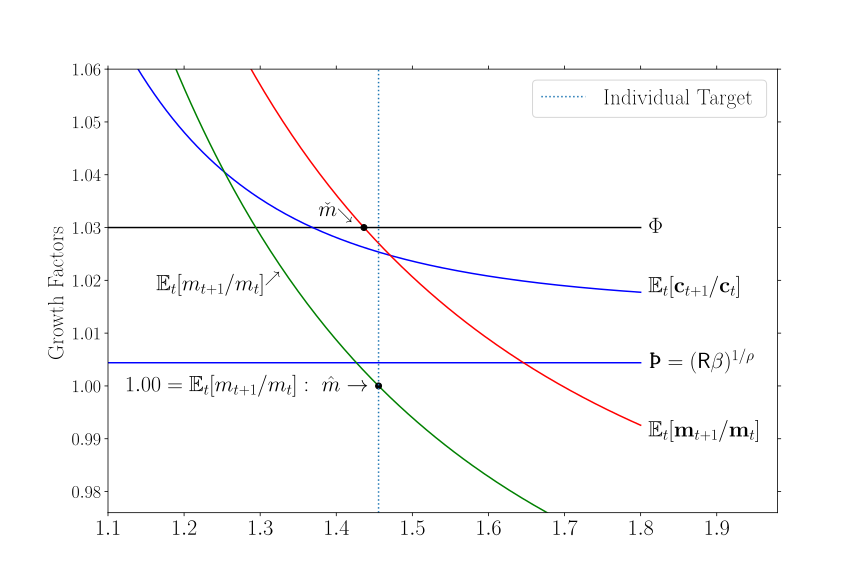
\includegraphics[width=0.8\linewidth]{\FigDir/cNrmTargetFig}} % Web 
\caption{`Stable' $\mNrm$ Values and Expected Growth Rates} % Web 
\label{fig:cNrmTargetFig} % Web
\end{figure} % Web
}{ % Web - no
\begin{figure}[tbp]
\centerline{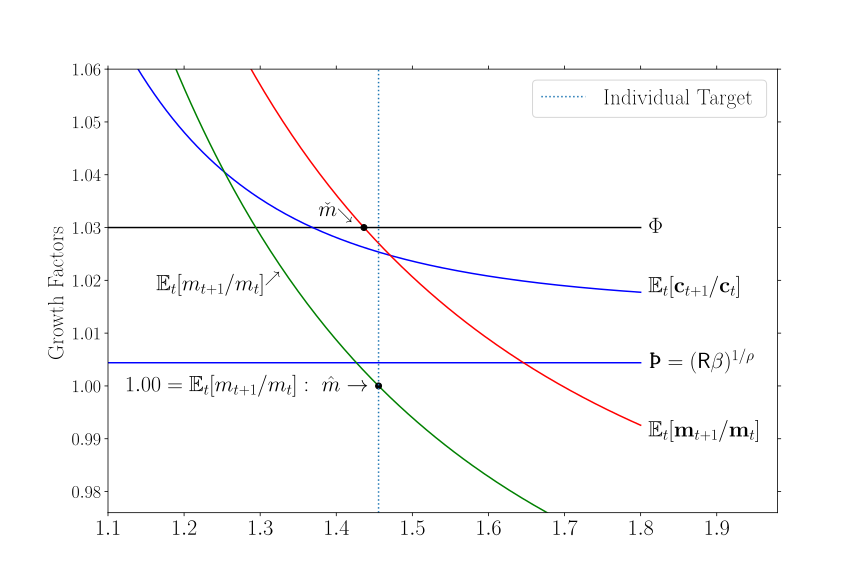
\includegraphics[width=0.8\textwidth]{\FigDir/cNrmTargetFig}}
\caption{Buffer Stock Target and Pseudo-Target}
\label{fig:cNrmTargetFig}
\end{figure}
} % Web


\begin{comment}
  Of course, the constraint never becomes irrelevant if human wealth is
  infinite.
We ruled out infinite human wealth at the beginning of this
  section by assuming $\Rfree> \PermGroFac$.
If this finite human wealth
  condition does not hold, it is possible to show that for any finite
  horizon consumer the marginal propensity to consume approaches the
  finite-horizon perfect foresight MPC as wealth approaches infinity.
  However, as the horizon gets longer, the perfect foresight MPC
  approaches zero.
It can be shown therefore that the limiting MPC for
  the converged consumption function approaches (but never reaches)
  zero.
(This is why we chose $\MPCminmin=0$ if the \FHWC~fails
  in the proofs above.)
\end{comment}

%\end{document}\endinput

\hypertarget{onetarget}{}
\hypertarget{Unique-Stable-Points}{}


\subsection{Unique `Stable' Points}\label{subsec:onetarget}\hypertarget{TheoremTarget}{}

One kind of `stable' point is a `target' value $\mTrgNrm$ such that if $\mNrm_{t}=\mTrgNrm$, then $\Ex_{t}[\mNrm_{t+1}]=\mNrm_{t}$.
Existence of such a target requires the \hyperlink{GICMod}{strong growth impatience} condition.

\begin{verbatimwrite}{Equations/TheoremMTargetIsStable}
  \begin{theorem}\label{thm:target} (Individual Market-Resources-to-Permanent-Income Ratio Target).
% Don't define it if already defined
    Consider the problem defined in Section~\ref{subsec:Setup}.
If \hyperlink{WRIC}{weak return impatience} (Assumption \ref{ass:WRIC}), \hyperlink{FVAC}{finite value of autarky} (Assumption \ref{ass:FVAC}) and \hyperlink{GICMod}{strong growth impatience} (Assumption \ref{ass:GICMod}) hold, then there exists $\mTrgNrm$, with $\mTrgNrm>0$, such that:
    \begin{equation}
      \Ex_t [{\mNrm}_{t+1}/\mNrm_t] = 1 \mbox{~if~} \mNrm_t = \mTrgNrm, 
      \label{eq:mTarget} % Don't define it if already defined
    \end{equation}
    and, 
    \begin{equation}
      \label{eq:stability} % Don't define it if already defined
      \begin{split}
        \forall {\mNrm}_t\in(0,\mTrgNrm),      \,\,& \Ex_t [{\mNrm}_{t+1}] > {\mNrm}_t  \\
        \forall {\mNrm}_t\in(\mTrgNrm,\infty), \,\,& \Ex_t [{\mNrm}_{t+1}] < {\mNrm}_t.
      \end{split}
    \end{equation}
  \end{theorem}
\end{verbatimwrite}
  \begin{theorem}\iflabelexists{thm:target}{}{\label{thm:target}} % Don't define it if already defined
    For the nondegenerate solution to the problem defined in Section~\ref{subsec:Setup} when {\FVAC}, {\WRIC}, and {\GICMod} all hold, there exists a unique cash-on-hand-to-permanent-income ratio $\mTrgNrm>0$ such that
    \begin{equation}
      \Ex_t [{\mNrm}_{t+1}/\mNrm_t] = 1 \mbox{~if~} \mNrm_t = \mTrgNrm.
      \iflabelexists{eq:mTarget}{}{\label{eq:mTarget}} % Don't define it if already defined
    \end{equation}
    Moreover, $\mTrgNrm$ is a point of `stability' in the sense that
    \begin{equation}
      \iflabelexists{eq:stability}{}{\label{eq:stability}} % Don't define it if already defined
      \begin{split}
        \forall {\mNrm}_t\in(0,\mTrgNrm),      \,\,& \Ex_t [{\mNrm}_{t+1}] > {\mNrm}_t  \\
        \forall {\mNrm}_t\in(\mTrgNrm,\infty), \,\,& \Ex_t [{\mNrm}_{t+1}] < {\mNrm}_t.
      \end{split}
    \end{equation}
  \end{theorem}


\begin{proof}\let\qed\relax
See Appendix \ref{subsubsec:AppxIndividTarget} for the proof.

\end{proof}


If $\mTrgNrm$ satisfies \eqref{eq:stability}, we say $\mTrgNrm$ is a point of `stability'.
%\end{document}\endinput

\hypertarget{mTargImplicit}{}
Since $\mNrm_{t+1}= (\mNrm_{t}-\cFunc(\mNrm_{t}))\RNrmByGRnd_{t+1}  +\tranShkAll_{t+1}$, the implicit equation for $\mTrgNrm$ becomes:
%
\begin{equation} \label{eq:mTargImplicit}
  \begin{split}
    \Ex_{t} [(\mTrgNrm-\cFunc(\mTrgNrm))\RNrmByGRnd_{t+1}+\tranShkAll_{t+1}] & = \mTrgNrm     \\   (\mTrgNrm-\cFunc(\mTrgNrm))\underbrace{\RNrmByG\Ex_{t}[\permShk^{-1}]}_{\colon = \bar{\RNrmByGRnd}}+1 & = \mTrgNrm .
  \end{split}
\end{equation}

\hypertarget{Collective-Stability}{}
\hypertarget{pseudo-steady-state}{}

The market-resources-to-permanent-income ratio target is the most restrictive among several competing definitions of stability.
Our least restrictive definition of `stability' derives from a traditional aggregate question in macro models: whether or not there is a `balanced growth' equilibrium in which aggregate variables (income, consumption, market resources) all grow by the same factor $\PermGroFac$.
In particular, if \hyperlink{GIC}{growth impatience} holds, the problem will exhibit a balanced-growth `pseudo-steady-state' point, by which we mean that there is some ${\mBalLvl}$ such that if $\mNrm_{t}>{\mBalLvl}$, then $\Ex_{t}[\mLvl_{t+1}/\mLvl_{t}] < \PermGroFac$.\hypertarget{balgrostable}{}
\hypertarget{balgrostableSolve}{}
Conversely if $\mNrm_{t}<{\mBalLvl}$ then $\Ex_{t}[\mLvl_{t+1}/\mLvl_{t}] > \PermGroFac$.
The target $\mBalLvl$ will be such that $\mLvl$ growth matches $\PermGroFac$, allowing us to write the implicit equation for $\mBalLvl$ as follows:
%
\begin{equation}\label{eq:balgrostable}
  \begin{split}
    \Ex_{t}[\mLvl_{t+1}]/\mLvl_{t} & =\Ex_{t}[\permLvl_{t+1}]/\permLvl_{t}
    \\  \Ex_{t}[\mNrm_{t+1}\PermGroFac\permShk_{t+1}\permLvl_{t}]/(\mNrm_{t}\permLvl_{t}) & =\Ex_{t}[\permLvl_{t}\PermGroFac\permShk_{t+1}]/\permLvl_{t}
    \\ \Ex_{t}\left[\permShk_{t+1}\underbrace{\left((\mNrm_{t}-\usual{\cFunc}(\mNrm_{t})\Rfree/(\PermGroFac\permShk_{t+1}))+\tranShkAll_{t+1}\right)}_{\mNrm_{t+1}}\right]/\mNrm_{t} & = 1
    \\ 
    \Ex_{t}\left[(\mBalLvl-\usual{\cFunc}(\mBalLvl))\overbrace{\Rfree/\PermGroFac}^{\RNrmByG}+\permShk_{t+1}\tranShkAll_{t+1}\right] & = \mBalLvl
    \\  (\mBalLvl-\usual{\cFunc}(\mBalLvl))\RNrmByG + 1 & = \mBalLvl .
  \end{split}
\end{equation}


The only difference between~\eqref{eq:balgrostable} and~\eqref{eq:mTargImplicit} is the substitution of $\RNrmByG$ for $\bar{\RNrmByGRnd}$.\footnote{A third `stable point' is the $\mBalLog$ where $\Ex_{t}[\log \mLvl_{t+1}] = \log \PermGroFac \mLvl_{t}$; this can be conveniently rewritten as $\Ex_{t}\left[\log\left((\mBalLog-\usual{\cFunc}(\mBalLog))\RNrmByGRnd+\permShk_{t+1}\tranShkAll_{t+1}\right)\right]  = \log \mBalLog_{t}$.
Because the expectation of the log of a stochastic variable is less than the log of the expectation, if a solution for $\mBalLog$ exists it will satisfy $\mBalLog > \mBalLvl$; in turn, if $\mTrgNrm$ exists, $\mTrgNrm>\mBalLog$.
The target $\mBalLog$ is guaranteed to exist when the \hyperlink{GICSdl}{log growth impatience} condition is satisfied (see below).
For our purposes, little would be gained by an analysis of this point parallel to those of the other points of stability; but to accommodate potential practical uses,  the {\ARKurl} toolkit computes the value of this point (when it exists) as \texttt{mBalLog}.}$^{,}$\footnote{Our choice to call to this the individual problem's `individual balanced-growth pseudo-steady-state' $\mBalLvl$ is motivated by what happens in the case where all draws of all future shocks just happen to take on their expected value of 1.0.
(They unexpectedly always take on their expected values).
In that infinitely improbable case, the economy \textit{would} exhibit balanced growth:
  \begin{align*}
    \Ex_{t}[\mNrm_{t+1}/\mNrm_{t}|\permShk_{t+1}=\tranShkAll_{t+1}=1] = \frac{\PermGroFac \left((\mBalLvl-\cFunc(\mBalLvl))\RNrmByG + 1 \right)}{\mNrm} = \PermGroFac.
  \end{align*}}
%Theorem~\ref{thm:MSSBalExists}~formally states the relevant proposition.
Under the weaker  \hyperlink{GIC}{growth impatience} condition, we can verify the existence of this pseudo-steady-state market resources to permanent income ratio, $\mBalLvl$.


\begin{verbatimwrite}{Equations/TheoremMSSBalExists}
  \begin{theorem}(Individual Balanced-Growth `Pseudo Steady State').
    \labelsafe{thm:MSSBalExists} % Don't define it if already defined
    Consider the problem defined in Section~\ref{subsec:Setup}.
If \hyperlink{WRIC}{weak return impatience} (Assumption \ref{ass:WRIC}), \hyperlink{FVAC}{finite value of autarky} (Assumption \ref{ass:FVAC}) and \hyperlink{GIC}{growth impatience} (Assumption \ref{ass:GICRaw}) hold, then there exists a unique $\mBalLvl$, with $\mBalLvl>0$ such that:
    \begin{equation}
      \Ex_t [\permShk_{t+1}{\mNrm}_{t+1}/\mNrm_t] = 1 \mbox{~if~} \mNrm_t = \mBalLvl.
      \label{eq:mBalLvl}
    \end{equation}
    Moreover, $\mBalLvl$ is a point of stability in the sense that:
    \begin{equation}
      \label{eq:stabilityStE}
      \begin{split}
        \forall {\mNrm}_t\in(0,\mBalLvl),      \,\,& \Ex_{t}[\mLvl_{t+1}]/\mLvl_{t} > \PermGroFac \\
        \forall {\mNrm}_t\in(\mBalLvl,\infty), \,\,& \Ex_{t}[\mLvl_{t+1}]/\mLvl_{t} < \PermGroFac.
      \end{split}
    \end{equation}
  \end{theorem}
\end{verbatimwrite}
  \begin{theorem}
    \iflabelexists{thm:MSSBalExists}{}{\label{thm:MSSBalExists}} % Don't define it if already defined
    For the nondegenerate solution to the problem defined in Section~\ref{subsec:Setup} when {\FVAC}, {\WRIC}, and {\GICRaw} all hold, there exists a unique pseudo-steady-state cash-on-hand-to-income ratio $\mBalLvl>0$ such that
    \begin{equation}
      \Ex_t [\PermShk_{t+1}{\mNrm}_{t+1}/\mNrm_t] = 1 \mbox{~if~} \mNrm_t = \mBalLvl.
      \iflabelexists{eq:mBalLvl}{}{\label{eq:mBalLvl}} % Don't define it if already defined
    \end{equation}
    Moreover, $\mBalLvl$ is a point of stability in the sense that
    \begin{equation}
      \iflabelexists{eq:stabilityStE}{}{\label{eq:stabilityStE}} % Don't define it if already defined
      \begin{split}
        \forall {\mNrm}_t\in(0,\mBalLvl),      \,\,& \Ex_{t}[\mLvl_{t+1}]/\mLvl_{t} > \PermGroFac \\
        \forall {\mNrm}_t\in(\mBalLvl,\infty), \,\,& \Ex_{t}[\mLvl_{t+1}]/\mLvl_{t} < \PermGroFac.
      \end{split}
    \end{equation}
  \end{theorem}

\begin{proof}
See Appendix \ref{subsubsec:AppxPseudoSS} for the proof.

\end{proof}


\begin{comment}
  \hypertarget{log-pseudo-steady-state}{}
  \subsubsection{The  expected `log-pseudo steady state'}\label{subsubsec:logpseudosteadystate}

  A final point of stability will be indicated by a $\sim$ accent; this is the $\mNrm$ at which the expectation of $\log \mLvl$ is unchanging.

  \begin{verbatimwrite}{Equations/TheoremGroIsStable}
    \begin{theorem}\label{thm:TheoremGroIsStable}{}{\label{thm:TheoremGroIsStable}}
      For the non-degenerate solution to Section~\ref{subsec:Setup}'s problem when {\FVAC}, {\WRIC}, and {\GICRaw} all hold, there exists a unique cash-on-hand-to-permanent-income ratio $\mBalLvl>0$ such that
      \begin{equation}
        \Ex_t [\log {\mLvl}_{t+1} ] = \log \mLvl_t \mbox{~if~} \mLvl_t = \mBalLvl.
        \label{eq:mTarget}
      \end{equation}
      Moreover, $\mBalLvl$ is a point of stability in the sense that
      \begin{equation} \label{eq:stabilityLog}
        \begin{split}
          \forall {\mNrm}_t\in(0,\mBalLvl),      \,\,& \Ex_t [\log {\mLvl}_{t+1}] > \log {\mLvl}_t  \\
          \forall {\mNrm}_t\in(\mBalLvl,\infty), \,\,& \Ex_t [\log {\mLvl}_{t+1}] < \log {\mLvl}_t.
        \end{split}
      \end{equation}
    \end{theorem}
  \end{verbatimwrite}
  \input{Equations/TheoremGroIsStable}

  with two associated Lemmas demonstrating that $\mBalLvl < \mBalLog$ and $\mBalLvl < \$\mTrgNrm$.
\end{comment}


\subsection{Example With Balanced-Growth \texorpdfstring{$\mBalLvl$}{m} But No Target~\texorpdfstring{$\mTrgNrm$}{m}}

Because the equations defining target and pseudo-steady-state $\mNrm$,~\eqref{eq:mTargImplicit} and~\eqref{eq:balgrostable}, differ only by substitution of $\RNrmByG$ for $\bar{\RNrmByGRnd}=\RNrmByG \Ex[\permShk^{-1}]$, if there are no permanent shocks ($\permShk \equiv 1$), the conditions are identical.
For many parameterizations (e.g., under the baseline parameter values used for constructing figure~\ref{fig:cNrmTargetFig}), $\mTrgNrm$ and $\mBalLvl$ will not differ much.

\renewcommand{\figFile}{GICModFailsButGICRawHolds}
\hypertarget{\figFile}{}
% Store the tex for standalone compilation
\ifthenelse{\boolean{Web}}{
\begin{figure}[tbp] % Web
\centerline{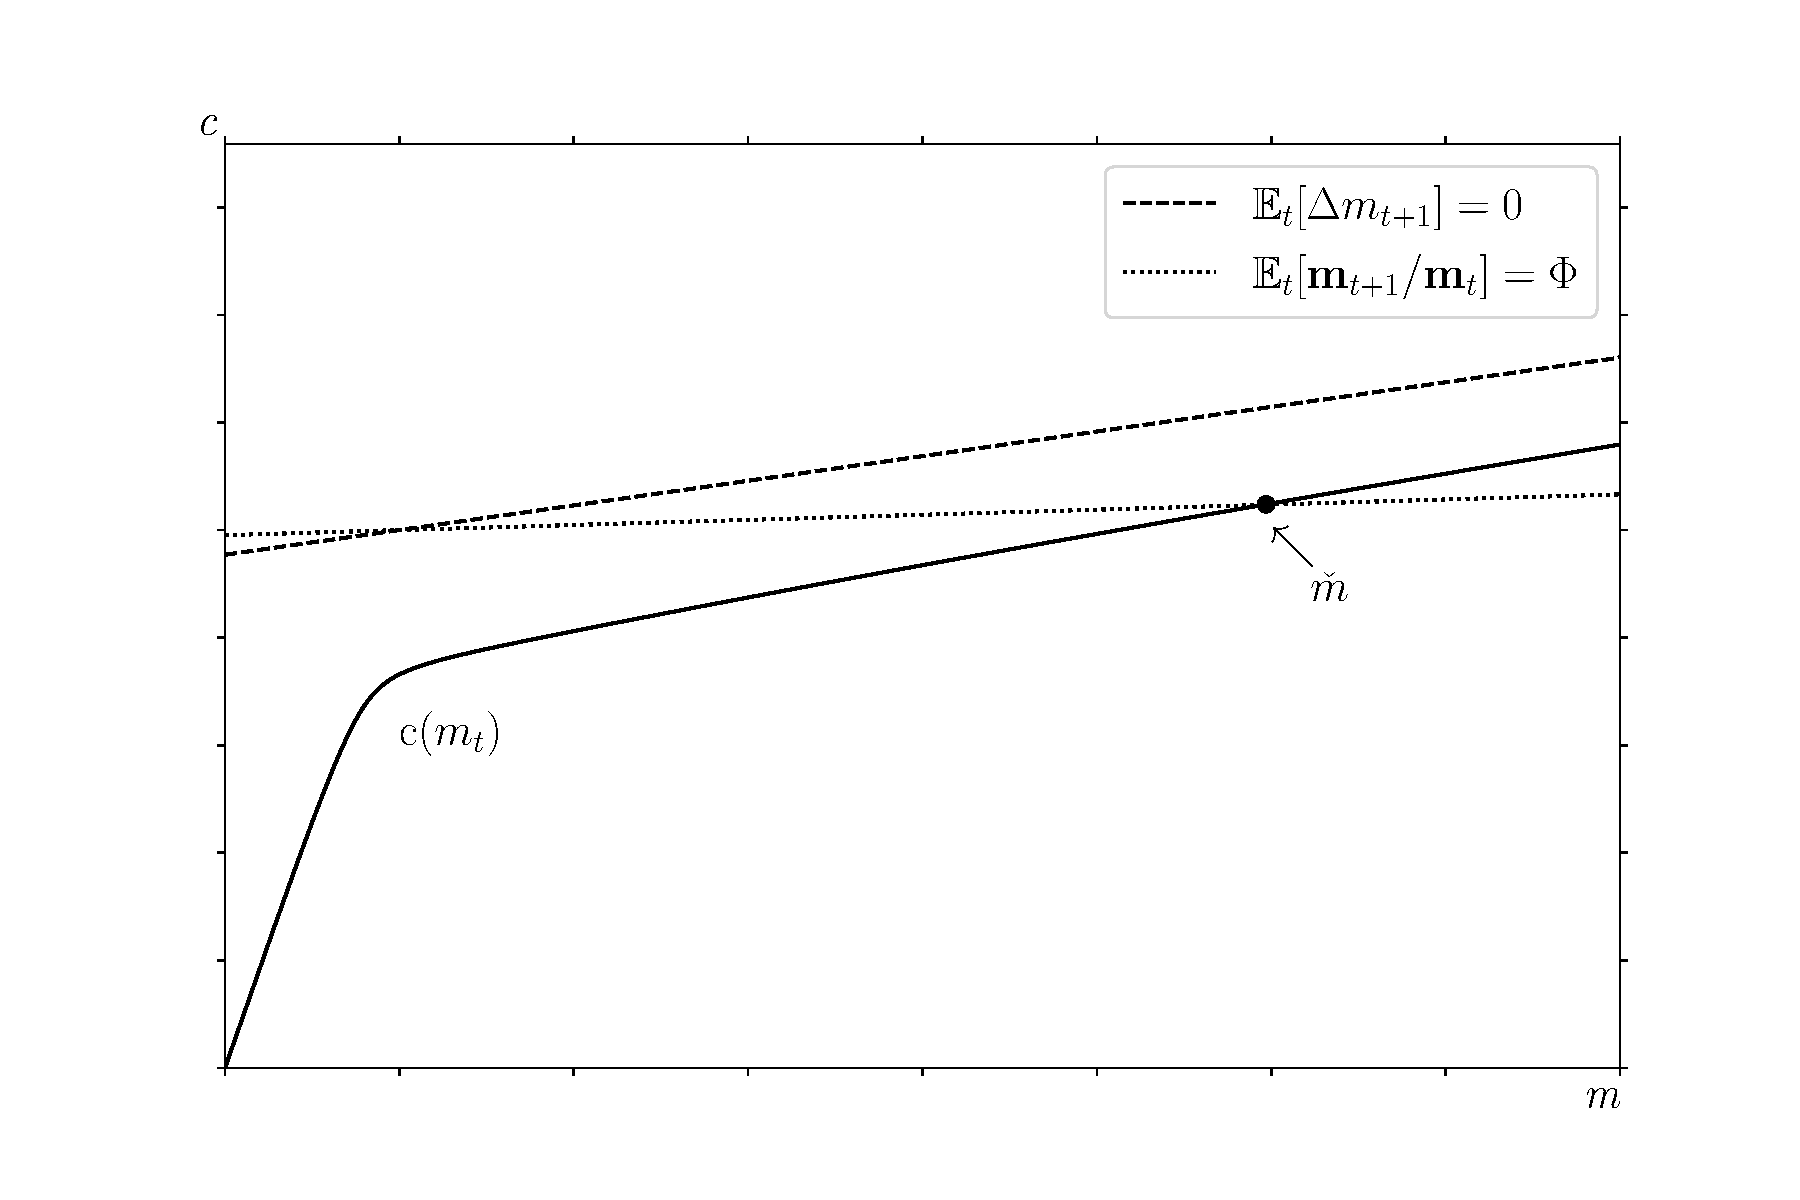
\includegraphics[width=0.8\textwidth]{\FigDir/GICModFailsButGICRawHolds}}
\caption{Convergence of the Consumption Rules} % Web 
\label{fig:GICModFailsButGICRawHolds}
\end{figure} % Web
}{ % Web - no
\begin{figure}[tbp]
\centerline{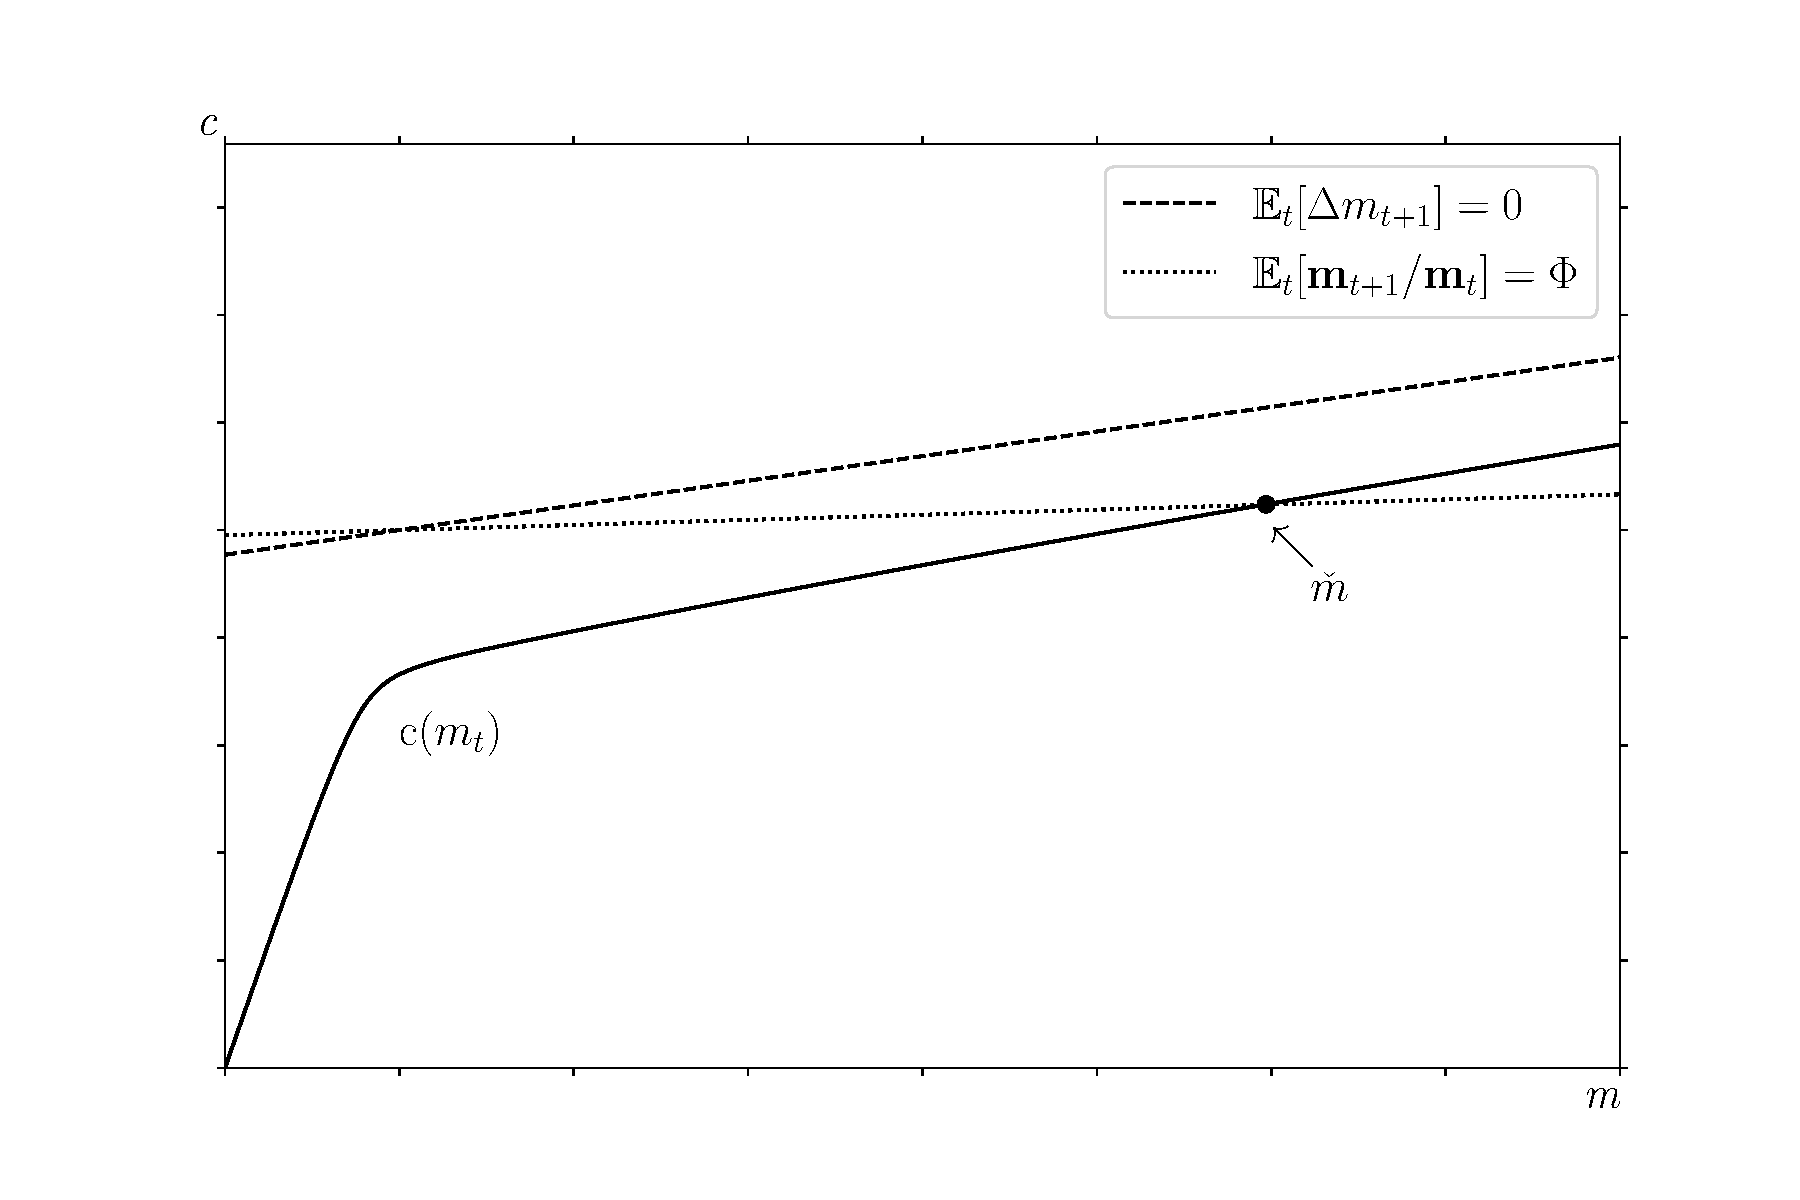
\includegraphics[width=6in]{\FigDir/GICModFailsButGICRawHolds}}
\caption{}
%\centering{\{{FVAC},{GIC},\cncl{GIC-Mod}\}: No $\TargetNrm{\mNrm}$ Exists But $\BalGroFac{\mNrm}$ Does}
\caption{Finite value of autarky and growth impatience hold but strong growth impatience fails: No Individaul Target Exists But Aggregate Target Does}
\label{fig:GICModFailsButGICRawHolds}
\end{figure}
} % Web - no


An illuminating exception is exhibited in Figure~\ref{fig:GICModFailsButGICRawHolds}, which modifies the baseline parameter values by quadrupling the variance of the permanent shocks, enough to cause failure of \hyperlink{GICMod}{strong growth impatience}; now there is no target level of market resources $\mTrgNrm$.
Nonetheless, the pseudo-steady-state still exists because it turns off realizations of the permanent shock.
It is tempting to conclude that the reason target $\mTrgNrm$ does not exist is that the increase in the size of the shocks induces a precautionary motive that increases the consumer's effective patience.
The interpretation is not correct because as market resources approach infinity, precautionary saving against noncapital income risk becomes negligible (as the proportion of consumption financed out of such income approaches zero).
The correct explanation is more prosaic: The increase in uncertainty boosts the expected uncertainty-modified rate of return factor from $\RNrmByG$ to $\bar{\RNrmByGRnd}>\RNrmByG$ which reflects the fact that in the presence of uncertainty the expectation of the inverse of the growth factor increases: $\PermGroFacAdj > \PermGroFac$.
That is, in the limit as $\mNrm \rightarrow \infty$ the increase in effective impatience reflected in $\GPFacMod < \GPFacRaw$ is entirely due to the certainty-equivalence growth adjustment, not to a (limiting) change in precaution.
In fact, the next section will show that an aggregate balanced growth equilibrium will exist even when realizations of the permanent shock are not turned off: The required condition for aggregate balanced growth is the regular \hyperlink{GIC}{growth impatience}, which ignores the magnitude of permanent shocks.\footnote{\cite{szeidlInvariant}'s impatience condition, discussed below, also tightens as uncertainty increases, but this is also not a consequence of a precaution-induced increase in patience -- it represents an increase in the tightness of the requirements of the `mixing condition' used in his proof.}

\begin{comment}
again, removed FHWC above since GIC holds.
double check.

\end{comment}

Before we get to the formal arguments, the key insight can be understood by considering an economy that starts, at date $t$, with the entire population at $\mNrm_{t}=\mBalLvl$, but then evolves according to the model's assumed dynamics between $t$ and $t+1$.
Equation~\eqref{eq:balgrostable} will still hold, so for this first period, at least, the economy will exhibit balanced growth: the growth factor for aggregate $\MLvl$ will match the growth factor for permanent income $\PermGroFac$.
It is true that there will be people for whom financial balances, $\bNrm_{t+1}$, where $\bNrm_{t+1} = \kNrm_{t+1}\Rfree/(\PermGroFac\permShk_{t+1})$, are boosted by a small draw of $\permShk_{t+1}$.
However, their contribution to the \textit{level} of the aggregate variable is given by $\bLvl_{t+1}=\bNrm_{t+1}\pLvl_{t}\permShk_{t+1}$, so their $\bNrm_{t+1}$ is reweighted by an amount that exactly unwinds that divisor-boosting.
This means that it is possible for the consumption-to-permanent-income ratio for every consumer to be small enough that their market resources ratio is expected to rise, and yet for the economy as a whole to exhibit a balanced growth equilibrium with a finite aggregate balanced growth steady state $\BalGroFac{\MNrm}$ (this is not numerically the same as the individual \hyperlink{pseudo-steady-state}{pseudo-steady-state} ratio $\mBalLvl$ because the problem's nonlinearities have consequences when aggregated).\footnote{Still, the pseudo-steady-state can be calculated from the policy function without any simulation, and therefore serves as a low-cost starting point for the numerical simulation process; see \href{https://econ-ark.org/materials/harmenberg-aggregation?launch}{Harmenberg-Aggregation} for an example.}


\begin{comment}
 **** candidate for deletion****
\hypertarget{LimitsAsmtToInfty}{}
\subsection{Limits as \texorpdfstring{$\mNrm$}{m} Approaches Infinity}\label{subsec:LimitsAsmtToInfty}

Define
\begin{align*}
  \Min{\cFunc}(\mNrm)  & = \MPCmin \mNrm
\end{align*}
which is the solution to an infinite-horizon problem with no noncapital income ($\tranShkAll_{t+n} = 0~\forall~n\geq1$); clearly $\Min{\cFunc}(\mNrm) < \usual{\cFunc}(\mNrm)$, since allowing the possibility of future noncapital income cannot reduce current consumption.
Our imposition of the {\RIC} guarantees that $\MPCmin > 0$, so this solution satisfies our definition of nondegeneracy, and because this solution is always available it defines a lower bound on both the consumption and value functions.%\footnote{We will assume the \RIC~holds here and subsequently so that $\MPCmin > 0$; the situation is a bit more complex when the \RIC~does not hold.  In that case the bound on consumption is given by the spending that would be undertaken by a consumer who faced binding liquidity constraints.}

Assuming the {\FHWC}~holds, the infinite-horizon perfect foresight solution~\eqref{eq:cFuncPFUnc} constitutes an upper bound on consumption in the presence of uncertainty, since the introduction of uncertainty strictly decreases the level of consumption at any $\mNrm$ (\cite{ckConcavity}).
Thus,
\begin{equation} \label{eq:lowerltupper}
  \begin{split}
    \Min{\cFunc}(\mNrm) < & \usual{\cFunc}(\mNrm)  < \bar{\cFunc}(\mNrm)  \\
    1 < & \usual{\cFunc}(\mNrm)/\Min{\cFunc}(\mNrm)  < \bar{\cFunc}(\mNrm)/\Min{\cFunc}(\mNrm).
  \end{split}
\end{equation}
But
\begin{align*}%  \label{eq:limitlowerupper}
  \lim_{m \rightarrow \infty} \bar{\cFunc}(\mNrm)/\Min{\cFunc}(\mNrm)
  & = \lim_{m \rightarrow \infty} (\mNrm -1+ \hNrm)/\mNrm  \\
  & = 1,
\end{align*}
so as $\mNrm \rightarrow \infty, \usual{\cFunc}(\mNrm)/\Min{\cFunc}(\mNrm) \rightarrow 1$, and the continuous differentiability and strict concavity of $\usual{\cFunc}(\mNrm)$ therefore implies
\begin{equation*} % \label{eq:limxtoinftycp}
  \lim_{m \rightarrow \infty} \usual{\cFunc}^{\prime}(\mNrm) =
  \Min{\cFunc}^{\prime}(\mNrm) = \bar{\cFunc}^{\prime}(\mNrm) = \MPCmin
\end{equation*}
because any other fixed limit would eventually lead to a level of consumption either exceeding $\bar{\cFunc}(\mNrm)$ or lower than $\Min{\cFunc}(\mNrm)$.
Figure~\ref{fig:mpclimits} illustrates these limits by plotting the numerical solution.


\hypertarget{LimitsAsmtToZero}{}
\subsection{Limits as \texorpdfstring{m}{m} Approaches Zero}
\label{subsec:LimitsAsmtToZero}

Equation~\eqref{eq:MPCmaxInvApndxIter} shows that the limiting value of
$\MPCmax$ is
\begin{align*}
  \MPCmax  & = 1-{\Rfree}^{-1}{(\pZero  \Rfree\DiscFac)}^{1/\CRRA}.
\end{align*}

Defining $\eFunc(\mNrm)=\cFunc(\mNrm)/\mNrm$ we have
\begin{align*}
  \lim_{m \rightarrow 0} \eFunc(\mNrm)  & = (1-\pZero^{1/\CRRA}\RPFac) = \MPCmax .
\end{align*}

Now using the continuous differentiability of the consumption function along with L'H\^opital's rule, we have
\begin{align*}
  \lim_{m \rightarrow 0} \usual{\cFunc}^{\prime}(\mNrm)  & = \lim_{m \rightarrow 0}
                                                          \eFunc(\mNrm) = \MPCmax.
\end{align*}

Figure~\ref{fig:mpclimits} visually confirms that the numerical solution obtains this limit for the MPC as $\mNrm$ approaches zero.
\end{comment}


\hypertarget{The-Aggregate-and-Idiosyncratic-Relationship-Between-Consumption-Growth-and-Income-Growth}{}
\section{Aggregate Invariant Relationships}
In this section, we move from characterizing the individual decision rule to properties of a distribution of individuals following the converged non-degenerate consumption rule $\cFunc$.
Assume a continuum of \textit{ex ante} identical buffer-stock households, with constant total mass normalized to one and indexed by $i$.
Szeidl~\citeyearpar{szeidlInvariant} proved that such a population, following the consumption rule $\cFunc$, will be characterized by invariant distributions of $\mNrm$, $\cNrm$, and $\aNrm$ under the log growth impatience condition:\footnote{\cite{szeidlInvariant}'s equation (9), in our notation, is:
  \begin{align*}
    \Ex \log \Rfree (1-\MPC) & < \Ex \log \PermGroFac \permShk
    \\  \Ex \log \Rfree \RPFac  &  < \Ex \log \PermGroFac \permShk
    \\ \log \GPFacRaw & < \Ex \log \permShk
  \end{align*}
  which, exponentiated, yields~\eqref{eq:GICSdl}.}
\hypertarget{GICSdl}{}
\begin{align}
   \log~\GPFacRaw & < \Ex [\log \permShk] \label{eq:GICSdl}
\end{align}
which is stronger than our \hyperlink{GICRaw}{growth impatience} ($\GPFacRaw < 1$), but weaker than our \hyperlink{GICMod}{strong growth impatience}  ($\GPFacMod < 1$).\footnote{Under our default (though not required) assumption that $\log \permShk \sim \mathcal{N}(-\sigma^{2}_{\permShk}/2,\sigma^{2}_{\permShk})$; \hyperlink{GICMod}{strong growth impatience} in this case, is $\GPFacRaw < \exp(-\sigma^{2})$, so if \hyperlink{GICMod}{strong growth impatience} holds then Szeidl's condition will hold.}

\hypertarget{Growth-Rates-of-Aggregate-Income-and-Consumption}{}

\cite{harmenbergInvariant} substitutes a clever change of probability-measure into Szeidl's proof, with the implication that under \hyperlink{GIC}{growth impatience}, invariant \emph{permanent-income-weighted} distributions of $\mNrm$ and $\cNrm$ exist.
In particular, let $\CDF_{\mNrm_{t},\permLvl_{t}}$ be the joint CDF of normalized market resources and permanent income at time $t$.\footnote{In the notation in \cite{harmenbergInvariant}, the \emph{permanent-income-weighted} measures are denoted as $\tilde{\psi}^{\mNrm}$.} The permanent-income-weighted CDF of $\mNrm_{t}$, $\Harm{\CDF}_{\mNrm_{t}}$, will be:
%
\begin{equation}\label{eq:HarmCDF}
\Harm{\CDF}_{\mNrm_{t}}(x) = \PermGroFac^{-t}\int_{0}^{x}\int_{0}^{\infty} \permLvl\CDF_{\mNrm_{t},\permLvl_{t}}(d\mNrm,d\permLvl)
\end{equation}

Simply put, the permanent-income-weighted CDF shows how the total `mass' of permanent income is distributed along normalized market resources.\footnote{The change of variables is analogous to weighting the mass of objects by coordinates and integrating to calculate the center of gravity.
\cite{wolf2021play} also use a similar approach to compare the relative dependence on labour and capital income across the wealth distribution.} The change of variables allows \cite{harmenbergInvariant} to prove a conjecture from an earlier draft of this paper (\cite{BufferStockTheoryQESubmit}) that under \hyperlink{GIC}{growth impatience}, aggregate consumption grows at the same rate $\PermGroFac$ as aggregate noncapital income in the long run (with the corollary that aggregate assets and market resources grow at that same rate).\hypertarget{test-Harmenbergs-method}{} \cite{harmenbergInvariant} also shows how the reformulation can reduce costs of calculation by over a factor of 100.\footnote{The Harmenberg method is implemented in the {\ARKurl}; see the last part of \href{https://github.com/econ-ark/BufferStockTheory/blob/master/Code/Python/test_Harmenbergs_method.sh}{\texttt{test\_Harmenbergs\_method.sh}}.
Confirming the computational advantage of Harmenberg's method, \href{https://econ-ark.org/materials/harmenberg-aggregation}{this notebook} finds that the Harmenberg method reduces the simulation size required for a given degree of accuracy by two orders of magnitude under the baseline parameter values defined above.} The remainder of this section draws out the implications of these points for aggregate balanced growth factors.



% Commented out text from the first part of this section is all collected below. 

% A large (infinite) collection of small (infinitesimal) buffer-stock consumers with identical parameter values can be thought of as a subset of the population within a single country (say, members of a given education or occupation group), or as the whole population in a small open economy with an exogenous (constant) interest rate.\footnote{It is also possible, and only slightly more difficult, to solve for the steady-state of a closed-economy version of the model where the interest rate is endogenous.}

% Until now for convenience we have assumed infinite-horizons, with the implicit understanding that white noise mortality could be handled by adjusting the effective discount factor.  On that basis, Section~\ref{subsec:cGroEqPermGroFacIndQ} continues to omit mortality.  But a reason mortality may be useful will appear at the end of Section~\ref{subsec:cGroEqPermGroFacQ}, so alternative mortality treatments are briefly examined in section~\ref{sec:Mortality-And-Redistribution}.

% Attanasio and Weber~\citeyearpar{aw95} point out that concavity of the consumption function can imply that it is quantitatively important to distinguish between the growth factor of average consumption and the average growth factor of  consumption.\footnote{Since we assume number of the households are   normalized to 1, aggregate and average variables are identical.}  We have just examined the average growth factor; we now examine the growth factor of the average.

% Microeconomic distributional relationships are increasingly central to macroeconomic research (see, e.g., \cite{violante_marginal_2021}'s recent Laffont lectures on relationship between the marginal propensity to consume and the distribution of assets).  But mapping from micro data to macro models can be subtle.  Hence this final section's aim of carefully describing those relationships in the paper's simple model.


%In a nutshell:\footnote{See \ref{sec:ApndxHarKmenberg} for a less abbreviated treatment in this paper's notation.} If $\permShk$ is described by density function $f_\permShk(\permShk)$, Harmenberg defines the \emph{permanent-income-neutral measure} by $\Harm{f}_\permShk(\permShk) \equiv \permShk f_\permShk(\permShk)$.  Following derivations parallel to those in the previous footnote, the condition for the existence of invariant permanent-income-weighted distributions is\hypertarget{GICHarm}{}
% \begin{align} 
%    \text{\GICHarm:~~} \log \GPFacRaw  & < \Harm{\Ex}[ \log \permShk] \label{eq:GICHarm}
% \end{align}
% where the {$\sim$} over the expectations operator indicates that the expectation is being taken with respect to $\Harm{f}_{\permShk}(\permShk)$.  Under our baseline assumption that the permanent shocks are lognormally distributed, it is possible to show that $\Harm{\Ex} [\log \permShk] = \permShkStd^{2}/2,$ so exponentiating both sides of this equation turns it into $\GPFacRaw < e^{\permShkVar/2}$ which is \textit{weaker} than the {\GICRaw} because $1 < e^{\permShkVar/2}$.\footnote{{\GICHarm} is always weaker than the {\GICRaw} because $x \log x$ is a convex function, so the expectation of the permanent-income-weighted distribution is always greater when there is risk than in the absence of risk (thanks again to the invaluable Mr Jensen).}$^{,}$\footnote{The fact that }


% Given the terminology developed earlier, the natural designation for the stable ratio of aggregate market resources to noncapital income is the `aggregate steady state' ratio, $\BalGroFac{M}$.  This is not numerically the same as the individual \hyperlink{pseudo-steady-state}{pseudo-steady-state} ratio $\mBalLvl$ because the nonlinearities involved in simulation and aggregation will have consequences.\footnote{Still, the pseudo-steady-state can be calculated immediately from the policy function without any simulation, and therefore would likely serve as an excellent and low-cost starting point for the numerical simulation process.}

% The idea also appears to be promisingly generalizable: For any statistic $\mathcal{S}$ that is the key focus of an analysis, it should be possible to improve the efficiency of simulations aimed at calculating that statistic by constructing an $\mathcal{S}$-weighted distribution rather than a neutral distribution.

%Such an economy will exhibit an \textit{aggregate} `steady-state' ratio of market resources to income $\MBalLvl$ (different from the individual `pseudo-steady-state' $\mBalLvl$).  Corresponding ratios for $\CLvl$ and other also exist even if the {\GICRaw} fails (so that the idiosyncratic pseudo-steady-state does not exist).


\hypertarget{Growth-Rates-of-Individual-Income-and-Consumption}{}
\subsection{Aggregate Balanced Growth of  Income, Consumption, and Wealth}\label{subsec:cGroEqPermGroFacQ}

Define $\Mean$ to yield the expected value operator with respect to the empirical distribution of a variable across the population (as distinct from the operator $\Ex$ which represents beliefs about the future for a given individual).\footnote{Formally, fix an individual $i$ and let $\{\tilde{c}^{i}_{t}\}_{t=0}^{\infty}$ and $\{\tilde{m}^{i}_{t}\}_{t=0}^{\infty}$ be a stochastic recursive sequence generated by the converged consumption rule as follows, $\tilde{c}^{i}_{t} = \cFunc(\tilde{\mNrm}^{i}_{t})$ and $\tilde{\mNrm}^{i}_{t+1} = \RNrmByGRnd^{i}_{t+1}(\tilde{\mNrm}^{i}_{t} -\cFunc(\tilde{\mNrm}^{i}_{t})) + \tranShkAll^{i}_{t+1}$, where the sequence of exogenous shocks are each defined on a \textit{theoretical probability space} $(\Omega, \Sigma, \mathbb{P})$.
Integration with respect to the measure $\mathbb{P}$ in the expected value operator $\Ex$ will be equivalent to \textit{empirical} integration $\mathbb{M}$ with respect to a suitable measure of agents on a nonatomic agent space.
In particular, for all $j$, $\Ex\gFunc(\tilde{\cNrm}_{t}^{j})  = \int \tilde{\cNrm}_{t}\,d\mathbb{P} =  \Mean\gFunc(\tilde{c}_{t})\colon = \int \gFunc(\tilde{\cNrm}_{t}^{i}) \lambda(di)$, where $\lambda$ is the measure of agents and  for any measurable function $\gFunc$.
For technical steps required to assert this claim, see \cite{Shanker2017a}, which utilizes  relatively recent results by \cite{Sun2009} and also the detailed construction by \cite{Cao2020}.} Using boldface capitals for aggregates, the growth factor for aggregate noncapital income becomes:
\begin{equation*}
  \YLvl_{t+1}/\YLvl_{t}  = \Mean\left[\tranShkAll_{t+1}\PermGroFac \permShk_{t+1}\permLvl_{t}\right]/\Mean\left[\permLvl_{t}\tranShkAll_{t}\right] = \PermGroFac
\end{equation*}
because of the independence assumptions we have made about the shocks $\tranShkAll$ and $\permShk$.

Consider an economy that satisfies the Szeidl impatience condition~\eqref{eq:GICSdl} and has existed for long enough by date~$t$ that we can consider it as Szeidl-converged.
In such an economy a microeconomist with a population-representative panel dataset could calculate the growth factor of consumption for each individual household, and take the average:
\begin{equation}\label{eq:MeanDeltaLogC}
  \begin{split}
    \Mean\left[\Delta \log \cLvl_{t+1}\right]  & = \Mean\left[ \log {\cNrm}_{t+1}\permLvl_{t+1} - \log c_{t}\permLvl_{t}\right]  \\
        %                            & = \Mean\left[ \log \permLvl_{t+1}- \log \permLvl_{t} + \log {\cNrm}_{t+1} - \log c_{t}\right]  \notag \\
    & = \Mean\left[ \log \permLvl_{t+1}- \log \permLvl_{t}\right] + \Mean\left[ \log {\cNrm}_{t+1} - \log c_{t}\right].
  \end{split}
\end{equation}

Because this economy is Szeidl-converged, distributions of $\cNrm_{t}$ and $\cNrm_{t+1}$ will be identical, so that the second term in  \eqref{eq:MeanDeltaLogC} disappears; hence, mean cross-sectional growth factors of consumption and permanent income are the same:
\begin{align}
  \Mean\left[\Delta \log \cLvl_{t+1}\right]  & = \Mean\left[ \Delta \log \permLvl_{t+1}\right] = \log \PermGroFac \label{eq:MeanDeltaLogCeqMeanDeltaLogP}.
\end{align}

In a Harmenberg-invariant economy (and therefore also any Szeidl-invariant economy), a similar proposition holds in the cross-section as a direct implication of the fact that a constant proportion of total permanent income is accounted for by the successive sets of consumers with any particular $\mNrm$ (recall Equation \eqref{eq:HarmCDF}).
This fact is one way of interpreting Harmenberg's definition of the density of the permanent-income-weighted invariant distribution of $\mNrm$; call this density~$\Harm{f}$.
To understand $\Harm{f}$, we can see how total aggregate market resources held by people with given $\mNrm$ will be:
%
%
\begin{equation}
\MLvl_{t}=\PermLvlAgg_{t}\Harm{f}(m)m
\end{equation}
%
%
By implication of Theorem \ref{thm:MSSBalExists}, $\MLvl_{t}$ grows at a rate $\PermGroFac$.
We will now use this property of $\Harm{f}$ to show that aggregate consumption also grows at rate $\PermGroFac$.
Call $\CLvl_{t}(\mNrm)$ the total amount of consumption at date $t$ by persons with market resources $\mNrm$, and note that in the invariant economy this is given by the converged consumption function $\cFunc(\mNrm)$ multiplied by the amount of permanent income accruing to such people $\Harm{f}(\mNrm)\PermLvlAgg_{t}$.
Since $\Harm{f}(\mNrm)$ is invariant and aggregate permanent income grows according to $\PermLvlAgg_{t+1} = \PermGroFac \PermLvlAgg_{t}$, for any $\mNrm$, the following characterizes the growth of total consumption:
%
%
\begin{equation*}
  \begin{split}
    \log \CLvl_{t+1}(\mNrm) - \log \CLvl_{t}(\mNrm) &  \notag
    = \log \cFunc(\mNrm) \Harm{f}(\mNrm)\PermLvlAgg_{t+1} - \log \cFunc(\mNrm)\Harm{f}(\mNrm)\PermLvlAgg_{t} \\
    & = \log \PermGroFac.
  \end{split}
\end{equation*}



\hypertarget{Balanced-Growth-Of-Covariances}{}
\subsection{Aggregate Balanced Growth and Idiosyncratic Covariances}\label{subsec:Covariances}

Harmenberg shows that the covariance between the individual consumption ratio $\cNrm$ and the idiosyncratic component of permanent income $\permLvl$ does not shrink to zero; thus, covariances are another potential measurement for construction of microfoundations.
% Here we draw out some of those implications.

Consider a date-$t$ Harmenberg-converged economy, and define the mean value of the consumption ratio as $\cNrmAvg_{t+n} \equiv \Mean[\cNrm_{t+n}]$.
Normalizing period-$t$ aggregate permanent income to $\PermLvlAgg_{t}=1$, total consumption at $t+1$ and $t+2$ are
\begin{equation}\label{eq:atp2vsatp1}
  \begin{split}
      %       \CLvl_{t}  % & l= \bar{\tilde{\cNrm}}_{t} = \Mean[\cNrm_{t}\permLvl_{t}] = \Mean[\cNrm_{t}]\Mean[\permLvl_{t}] + \cov_{t}(\cNrm_{t}, \permLvl_{t}) \\
        %                            & = %\bar{\tilde{\cNrm}}_{t} =
                                       %                                        \Mean[\cNrm_{t}\permLvl_{t}] = \Mean[\cNrm_{t}]\overbrace{\Mean[\permLvl_{t}]}^{=1} + \cov_{t}(\cNrm_{t}, \permLvl_{t})  \\
    \CLvl_{t+1} & = \Mean[\cNrm_{t+1}\permLvl_{t+1}] = \cNrmAvg_{t+1}\PermGroFac^{1} + \cov_{t+1}(\cNrm_{t+1}, \permLvl_{t+1})
    \\  \CLvl_{t+2} & = \Mean[\cNrm_{t+2}\permLvl_{t+2}] = \cNrmAvg_{t+2}\PermGroFac^{2} + \cov_{t+2}(\cNrm_{t+2}, \permLvl_{t+2})
  \end{split}
\end{equation}
and Harmenberg's proof that $\CLvl_{t+2}-\PermGroFac \CLvl_{t+1}=0$ allows us to obtain:
\begin{equation} \label{eq:cNrmvsCov}\begin{split}
                      %                       0 & = \cNrmAvg_{t+2}\PermGroFac^{2} + \cov_{t+2}-\PermGroFac\left(\PermGroFac\cNrmAvg_{t+1} + \cov_{t+1}\right)\\ %
        %         \cNrmAvg_{t+2}\PermGroFac^{2} + \cov_{t+2}   & =\cNrmAvg_{t+1}\PermGroFac^{2} + \PermGroFac \cov_{t+1}\\
    \left(\cNrmAvg_{t+2} - \cNrmAvg_{t+1}\right)\PermGroFac^{2} & = \PermGroFac \cov_{t+1} - \cov_{t+2} .
  \end{split}\end{equation}

In a Szeidl-invariant economy, $\cNrmAvg_{t+2} = \cNrmAvg_{t+1}$, so the economy exhibits balanced growth in the covariance:
\begin{align}
  \cov_{t+2} & = \PermGroFac \cov_{t+1}.
\end{align}

The more interesting case is when the economy is Harmenberg- but not Szeidl-invariant.
In that case, if the $\cov$ and the $\cNrmAvg$ terms have constant growth factors $\GroFac_{\cov}$ and $\GroFac_{\cNrmAvg}$,\footnote{This `if' is a conjecture, not something proven by Harmenberg (or anyone else).
But see appendix~\ref{sec:ApndxBalancedGrowthcNrmAndCov} for an example of a Harmenberg-invariant economy in which simulations suggest this proposition holds.} an equation corresponding to \eqref{eq:cNrmvsCov} will hold in $t+n$:
\begin{equation} \label{eq:aNrmGrovsCovGronm1}
  \begin{split}
    (\overbrace{\GroFac_{\cNrmAvg}^{n}\cNrmAvg_{t}}^{\cNrmAvg_{t+n}}-\GroFac^{n-1}_{\cNrmAvg}\cNrmAvg_{t})\PermGroFac^{n} & = \left(\PermGroFac\GroFac_{\cov}^{n-1} -\GroFac_{\cov}^{n}\right)\cov_{t}
    \\ (\GroFac_{\cNrmAvg}\PermGroFac)^{n-1} (\GroFac_{\cNrmAvg}-1)\cNrmAvg_{t}\PermGroFac & = \GroFac_{\cov}^{n-1}(\PermGroFac - \GroFac_{\cov}) \cov_{t}
  \end{split}
\end{equation}
so for the LHS and RHS to grow at the same rates we need
\begin{align}
  \GroFac_{\cov}  & = \GroFac_{\cNrmAvg}\PermGroFac \label{eq:aNrmGrovscovGro}.
\end{align}
This is intuitive:  In the Szeidl-invariant economy, it just reproduces our result above that the covariance exhibits balanced growth because $\GroFac_{\cNrmAvg}=1$.
The revised result just says that in the Harmenberg case where the mean value $\cNrmAvg$ of the consumption ratio $\cNrm$ can grow, the covariance must rise in proportion to any ongoing expansion of $\cNrmAvg$ (as well as in proportion to the growth in $\permLvl$).

\begin{comment}
  \begin{align*}
    \overbrace{\GroFac_{\cNrmAvg}^{n} \cNrmAvg_{t}}^{\cNrmAvg_{t+n}}(\GroFac_{\cNrmAvg} - 1)\PermGroFac^{n} & =(\GroFac_{\cov} - \PermGroFac) \overbrace{\cov_{t}\GroFac_{\cov}^{n}}^{\cov_{t+n}}
    \\
    (\GroFac_{\cNrmAvg}\PermGroFac/\GroFac_{\cov})^{n} \cNrmAvg_{t}(\GroFac_{\cNrmAvg} - 1) & =(\GroFac_{\cov} - \PermGroFac) \cov_{t}
  \end{align*}
  and a corresponding equation will hold in $t+1$:
  \begin{align*}
    \\  \overbrace{\GroFac_{\cNrmAvg} \cNrmAvg_{t}}^{\cNrmAvg_{t+1}}(\GroFac_{\cNrmAvg} - 1)\PermGroFac & =(\GroFac_{\cov} - \PermGroFac) \overbrace{\cov_{t}\GroFac_{\cov}}^{\cov_{t+1}}
  \end{align*}
  \begin{align*}
    (\GroFac_{\cNrmAvg} - 1)\cNrmAvg_{t}(\GroFac_{\cNrmAvg} - 1)\PermGroFac & =(\GroFac_{\cov} - \PermGroFac) \cov_{t}(\GroFac_{\cov} - 1)
  \end{align*}

  \begin{align*}
    (\GroFac_{\cNrmAvg} - 1)\cNrmAvg_{t}(\GroFac_{\cNrmAvg} - 1)\PermGroFac & =(\GroFac_{\cov} - \PermGroFac) \cov_{t}(\GroFac_{\cov} - 1)
  \end{align*}
  \begin{align}
                                                                              %                                                                               \GroFac_{\cNrmAvg} - 1 & = \GroFac_{\cov} - \PermGroFac \\
        %         \GroFac_{\cNrmAvg} + \PermGroRte & = \GroFac_{\cov}  \\
    \GroFac_{\cov} & = \GroFac_{\cNrmAvg} + (\PermGroFac - 1) \label{eq:aNrmGroVscov}
  \end{align}
  \begin{align*}
    \CLvl_{t}  % & l= \bar{\tilde{\cNrm}}_{t} = \Harm{\Mean}_{t+1}[\cNrm_{t}\permLvl_{t}] = \Harm{\Mean}_{t+1}[\cNrm_{t}]\Harm{\Mean}_{t+1}[\permLvl_{t}] + \cov_{t}(\cNrm_{t}, \permLvl_{t}) \\
                 & = %\bar{\tilde{\cNrm}}_{t} =
                   \Harm{\Mean}_{t\phantom{+1}}[\cNrm]\phantom{\PermGroFac} = \Mean[\cNrm_{t\phantom{t+1}}]\phantom{\PermGroFac} + \cov_{t}(\cNrm_{t}, \permLvl_{t})  \\
    \CLvl_{t+1} & = \Harm{\Mean}_{t         +1 }[\cNrm]         \PermGroFac  = \cNrmAvg_{t+1}\PermGroFac  + \cov_{t+1}(\cNrm_{t+1}, \permLvl_{t+1})
  \end{align*}

  Still, both of these quantitites are in priniciple measurable in microdata.
%Indeed, in principle, the Harmenberg-invariant distribution itself could be measured in such data.

\end{comment}

\begin{comment}
  which is the point where $\HarmWide{\cov}_{t}$ is the covariance calculated according to the Harmenberg measure.

  As Harmenberg points out, a convenient feature of his measure is that $\Harm{\Mean}_{t+n}[\permLvl_{t+n}]=\PermGroFac^{n}$.
Using this, if by date $t=0$ the economy had achieved a Harmenberg-invariant state then we could define $\cNrmAvg=\Harm{\Mean}_{t}[\cNrm_ {t}]$ and use the fact that thereafter assets grow at the constant rate $\PermGroFac$ to obtain
  \begin{equation}
    \begin{split}\label{eq:covProblem}
      \CLvl_{t+1} & = \PermGroFac \CLvl_{t}\notag \\
      \cNrmAvg\PermGroFac +\HarmWide{\cov}(\cNrm_{t+1},\permLvl_{t+1})   & = \PermGroFac \left( \cNrmAvg    +  \HarmWide{\cov}(\cNrm_{t},\permLvl_{t})\right)
      \\  \HarmWide{\cov}(\cNrm_{t+1},\permLvl_{t+1})   & = \HarmWide{\cov}(\cNrm_{t},\permLvl_{t})  \notag
    \end{split}
  \end{equation}

  A corresponding argument shows that $\cov(\mNrm,\permLvl)$ also grows by $\PermGroFac$.
\end{comment}


\hypertarget{microfounding-macro-needs-ergodicity}{}
\subsection{Implications for Microfoundations}\label{subsec:microfoundations}

Thus we have microeconomic propositions, for both growth factors and for covariances of observable variables,\footnote{Parallel results to those for consumption can be obtained for other measures like market assets.} that can be tested in either cross-section or panel microdata to judge (and calibrate) the microfoundations that should hold for any macroeconomic analysis that requires balanced growth for its conclusions.

At first blush, these points are reassuring; one of the most persuasive arguments for the agenda of building microfoundations of macroeconomics is that newly available `big data' allow us to measure cross-sectional covariances with great precision, so that we can use microeconomic natural experiments to disentangle questions that are hopelessly entangled in aggregate time-series data.
Knowing that such covariances ought to be a stable feature of a stably growing economy is therefore encouraging.

But this discussion also highlights an uncomfortable point: In the model as specified, permanent income does not have a limiting distribution; it becomes ever more dispersed as the economy with infinite-horizon consumers continues to exist indefinitely.

A few microeconomic data sources attempt direct measurement of `permanent income'; \cite{cstwMPC}, for example, show that their assumptions about the magnitude of permanent shocks (and mortality; see below) yield a simulated distribution of permanent income that roughly matches answers in the U.S.\ \emph{Survey of Consumer Finances} (`SCF') to a question designed to elicit a direct measure of respondents' permanent income.
They use those results to calibrate a model to match empirical facts about the distribution of permanent income and wealth, showing that the model also does fits empirical facts about the marginal propensity to consume.
The quantitative credibility of the argument depends on the model's match to the distribution of permanent income inequality, which would not be possible in a model without a non-degenerate steady-state distribution of permanent income.

For macroeconomists who want to build microfoundations by comparing the microeconomic implications of their models to micro data (directly -- not in ratios to difficult-to-meaure `permanent income'), it would be something of a challenge to determine how to construct empirical-data-comparable simulated results from a model with no limiting distribution of permanent income.

\begin{comment}
  \hypertarget{Consumption-and-Income-Growth-at-the-Household-Level}{}
  \subsection{Identical Growth in Income, Consumption, and Wealth}\label{subsec:cGroEqPermGroFacIndQ}

  Unfortunately, the \hyperlink{GICMod}{strong growth impatience} condition that we imposed which yielded all of these intuitive propositions at once is rather restrictive.
Modeling experience indicates that it is not always possible to find plausible combinations of parameter values that satisfy that condition.
Furthermore, while the {\GICRaw} is a considerably looser condition, as noted above (and as

  % The foregoing analysis is motivated by the emerging realization of the importance of understanding of covariance relationships in microeconomic populations (between the marginal propensity to consume and the level of wealth, e.g.).
\end{comment}

Death can solve this problem.


\hypertarget{Mortality}{}
\subsection{Mortality Yields Invariance}\label{sec:Mortality}

\hypertarget{Blanchard-Lives}{}
Most heterogeneous-agent models incorporate a constant positive probability of death, following \cite{blanchardFinite} and \cite{yaari1965uncertain}.
In the Blanchardian model, if the probability of death exceeds a threshold that depends on the size of the permanent shocks,~\cite{cstwMPC} show that the limiting distribution of permanent income has a finite variance.
\cite{blanchardFinite} assumes a universal annuitization scheme in which estates of dying consumers are redistributed to survivors in proportion to survivors' wealth, giving the recipients a higher effective rate of return.
This treatment has considerable analytical advantages, most notably that the effect of mortality on the time preference factor is the exact inverse of its effect on the (effective) interest factor.
That is, if the `pure' time preference factor is $\DiscFacRaw$ and probability of remaining alive (not dead) is $\Alive$, then the assumption that no utility accrues after death makes the effective discount factor $\DiscFacLiv=\DiscFacRaw\Alive$  while the enhancement to the rate of return from the annuity scheme yields an effective interest factor $\RfreeEff=\Rfree/\Alive$ (recall that because of white-noise mortality, the average wealth of the two groups is identical).
Combining these, the effective patience factor in the new economy $\DiscFacLiv \RfreeEff$ is unchanged from its value in the infinite-horizon model:% chktex 2
\begin{equation}
  \DiscFacLiv \RfreeEff = {\left(\DiscFac \Alive \Rfree / \Alive\right)}^{1/\CRRA} = {\left(\Rfree \DiscFacRaw\right)}^{1/\CRRA} = \APFac.
\end{equation}

The only adjustments this requires to the analysis above are therefore to the few elements that involve a role for the interest factor distinct from its contribution to $\APFac$ (principally, the {\RIC}, which becomes $\APFac/\RfreeEff$).
%These would need to be adjusted to incorporate in interest factor with a higher rate of return.  %For example, the {\RIC}~($\APFac/(\Rfree /\Alive) < 1$) will be somewhat easier to satisfy because $\Rfree/\Alive > \Rfree$.

% The numerical finding that the covariance term above is approximately zero allows us to conclude again that the key requirement for aggregate balanced growth is presumably the {\GICRaw}.

\hypertarget{Modigliani-Lives}{}

\cite{blanchardFinite}'s innovation was valuable not only for the insight it provided but also because when he wrote, the principal alternative, the Life Cycle model of~\cite{modiglianiWealth}, was computationally challenging given then-available technologies.
Despite its (considerable) conceptual value, Blanchard's analytical solution is now rarely used because essentially all modern modeling incorporates uncertainty, constraints, and other features that rule out analytical solutions anyway.% chktex 2  %Modern models can can easily handle assumptions more realistic than Blanchard's about the disposition of assets at death.

The simplest alternative to Blanchard is to follow Modigliani in constructing a realistic description of income over the life cycle and assuming that any wealth remaining at death occurs accidentally (not implausible, given the robust finding that for the great majority of households, bequests amount to less than 2 percent of lifetime earnings,~\cite{hendricksBequests,hendricksSmallBequests}).

Even if bequests are accidental, a macroeconomic model must make some assumption about how they are disposed of: As windfalls to heirs, estate tax proceeds, etc.
We again consider the simplest choice, because it represents something of a polar alternative to Blanchard.
Without a bequest motive, there are no behavioral effects of a 100 percent estate tax; we assume such a tax is imposed and that the revenues are effectively thrown in the ocean:  The estate-related wealth effectively vanishes from the economy.

The chief appeal of this approach is the simplicity of the change it makes in the condition required for the economy to exhibit a balanced growth equilibrium (for consumers without a life cycle income profile).
If $\Alive$ is the probability of remaining alive, the condition changes from the plain \hyperlink{GIC}{growth impatience} to a looser mortality-adjusted version of \hyperlink{GIC}{growth impatience}:
\hypertarget{GICLivModDefn}{}
\begin{align}
  \Alive  \APFac_{\PermGroFac} & < 1. \label{eq:GICLivMod}
\end{align}

With no income growth, what is required to prohibit unbounded growth in aggregate wealth is the condition that prevents the per-capita wealth-to-permanent-income ratio of surviving consumers from growing faster than the rate at which mortality diminishes their collective population.
With income growth, the aggregate wealth-to-income ratio will head to infinity only if a cohort of consumers is patient enough to make the desired rate of growth of wealth fast enough to counteract combined erosive forces of mortality and productivity.

\hypertarget{Discussion-Growth-Impatience}{}
\section{Consumer Patience and Limiting Consumption}\label{sec:GICdiscussion}

\renewcommand{\figName}{cFuncsConverge} 
 % Store the tex for standalone compilation
 \ifthenelse{\boolean{Web}}{
\begin{figure}[tbp] % Web
\centerline{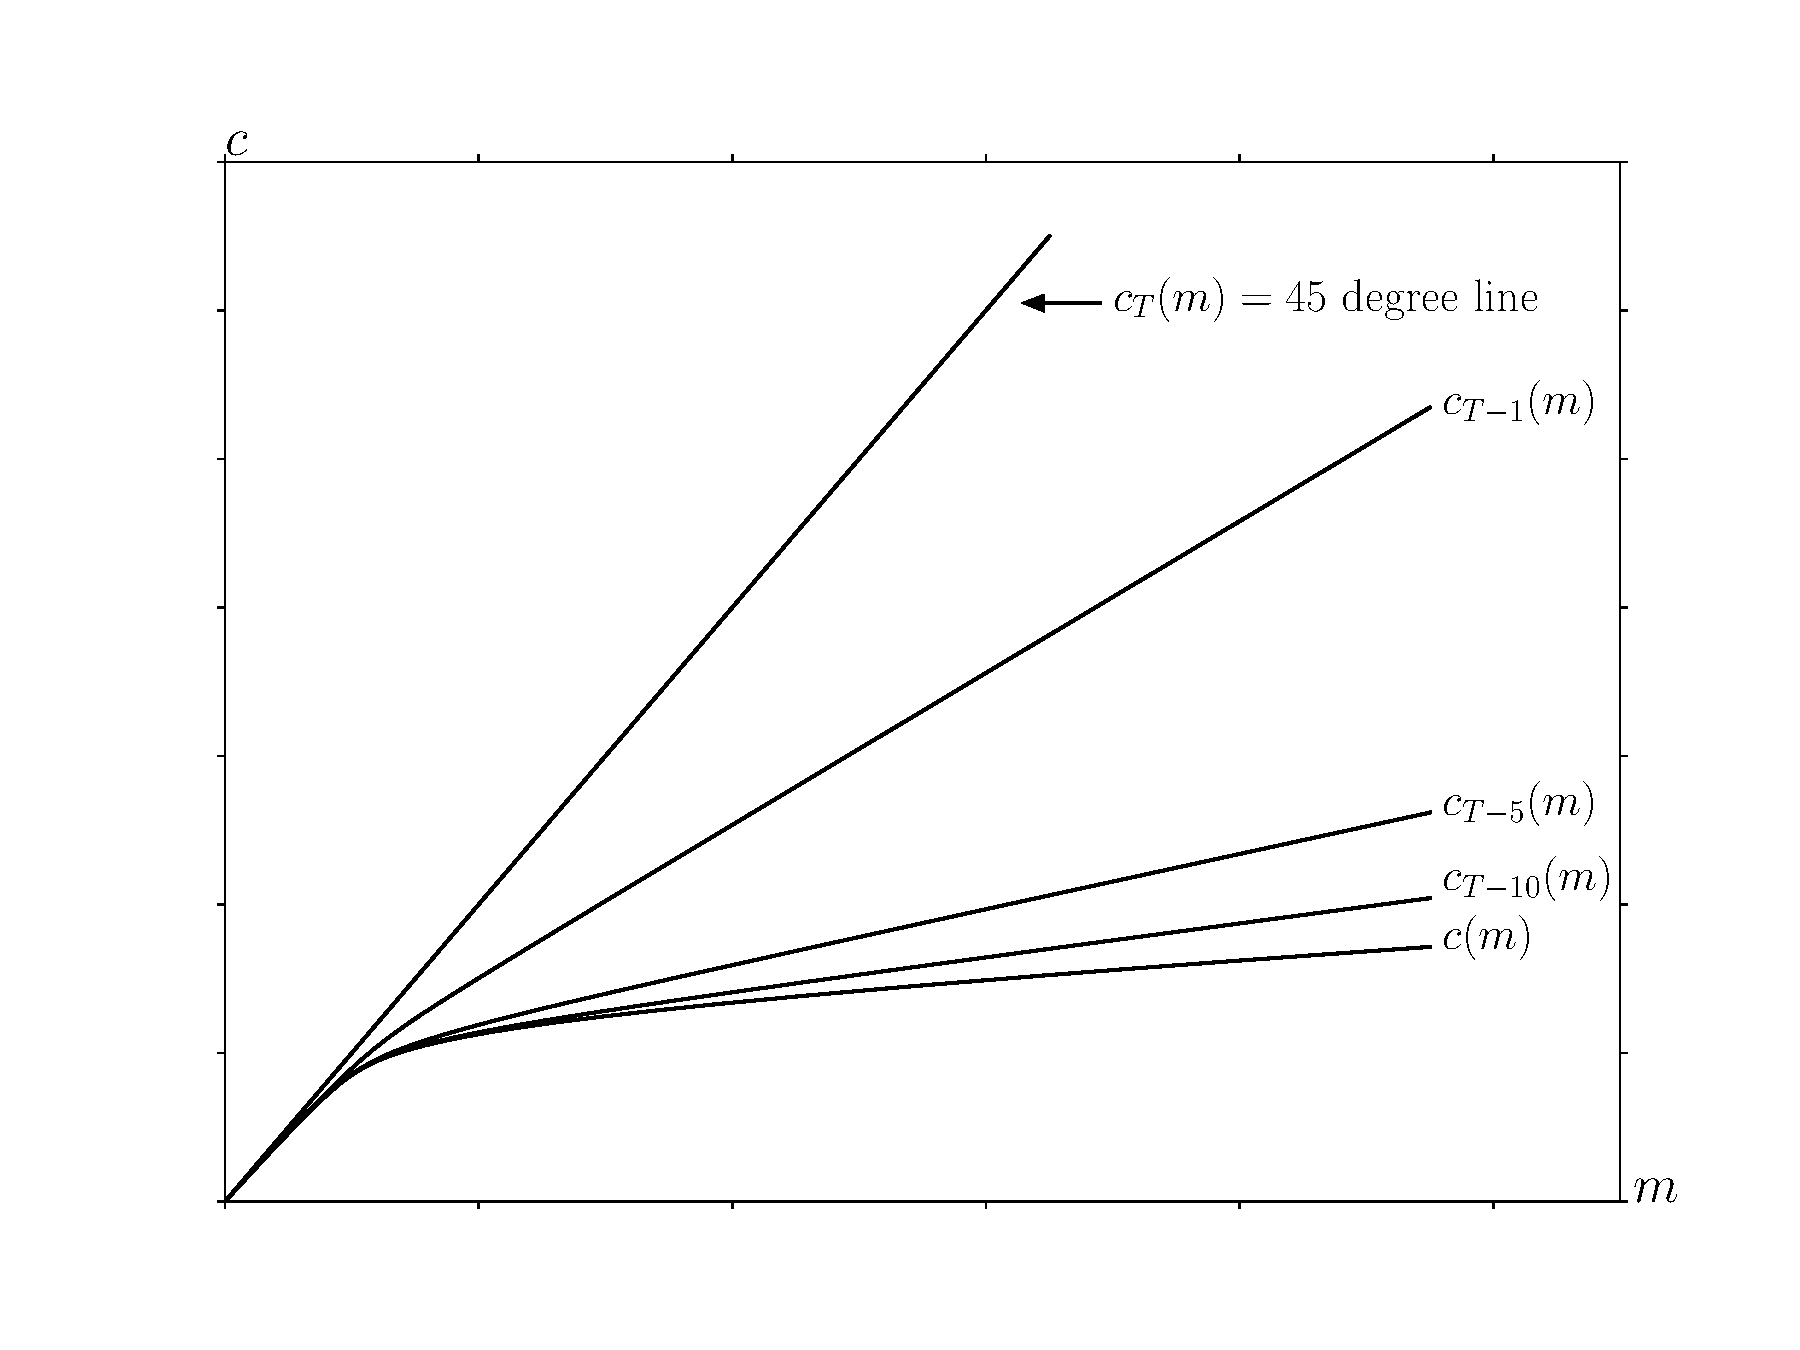
\includegraphics[width=0.7\linewidth]{\FigDir/cFuncsConverge}} % Web 
\caption{Convergence of the Consumption Rules} % Web 
\label{fig:cFuncsConverge} % Web 
\end{figure} % Web
}{ % Web - no
\begin{figure}[tbp]
\centerline{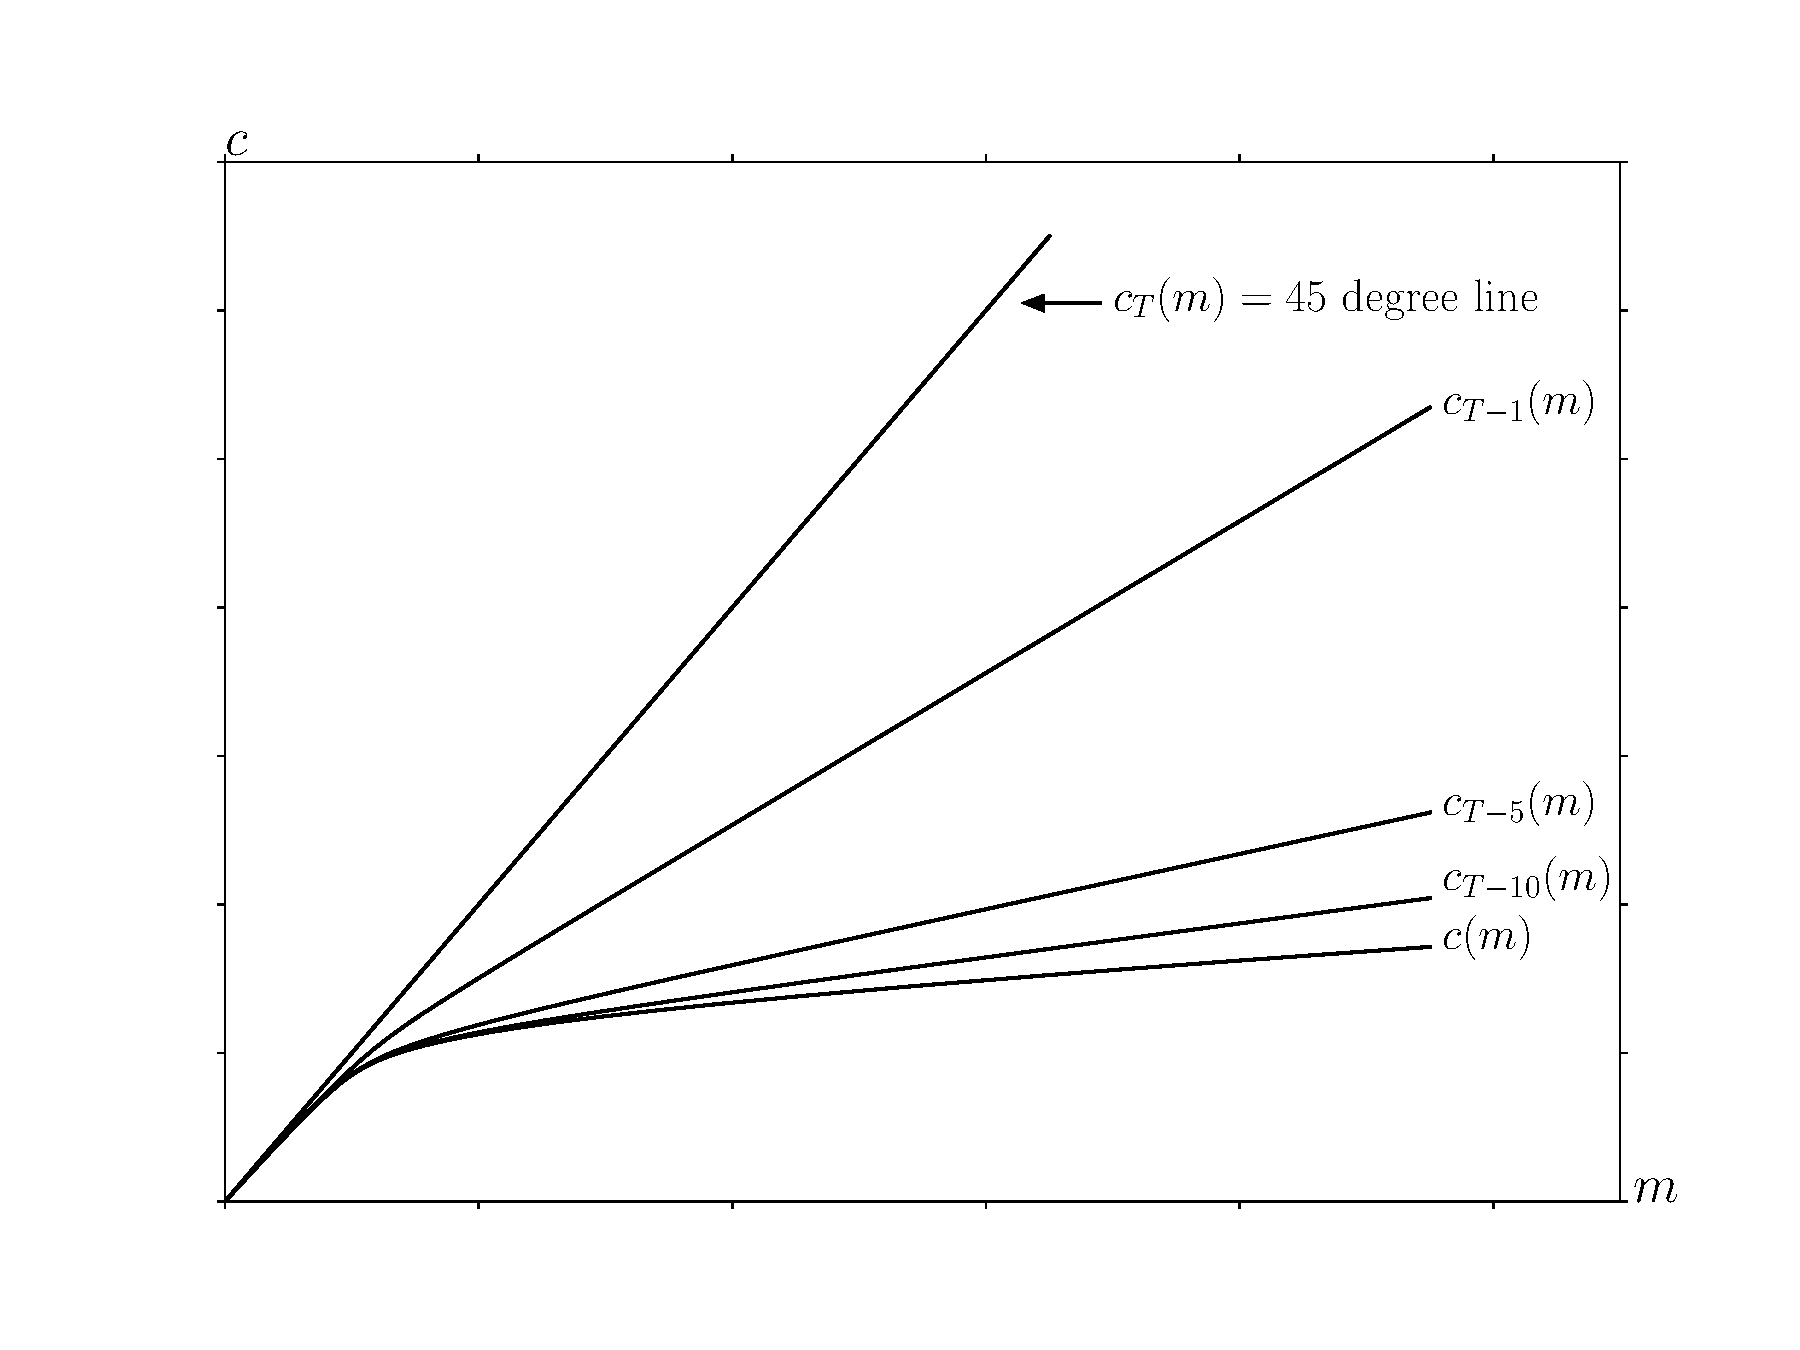
\includegraphics[width=5.25in]{\FigDir/cFuncsConverge}}
\caption{Convergence of the Consumption Rules}
\label{fig:cFuncsConverge}
\end{figure}
} % Web - no
 

Having established our formal results, we are ready to describe how the various patience conditions determine the characteristics of the limiting consumption function.
To fix ideas, we start with a quantitative example using the familiar benchmark case where \hyperlink{RIC}{return impatience}, \hyperlink{GIC}{growth impatience} and \hyperlink{FHWC}{finite human wealth} all hold, shown by Figure~\ref{fig:cFuncsConverge}.
The figure depicts the successive consumption rules that apply in the last period of life $(\cFunc_{T})$, the second-to-last period, and earlier periods under parameter values listed in Table~\ref{table:Calibration}.
(The 45 degree line is $\cFunc_{T}(\mNrm) = m$ because in the last period of life it is optimal to spend all remaining resources.)

Under the same parameter values, Figures~\ref{fig:mpclimits}--\ref{fig:cFuncBounds} capture the theoretical bounds and MPCs of the converged consumption rule.
In Figure~\ref{fig:mpclimits}, as $\mNrm$ rises, the marginal propensity to consume approaches $\MPCmin=(1-\RPFac)$ as $m \rightarrow \infty$, the same as the perfect foresight MPC.
Moreover, as $\mNrm$ approaches zero, the MPC approaches $\MPCmax=(1-\pZero^{1/\CRRA}\RPFac)$.


\renewcommand{\figFile}{mpclimits}
\hypertarget{\figFile}{}
\hypertarget{MPCLimits}{}
 \ifthenelse{\boolean{Web}}{
\begin{figure} % Web
\centerline{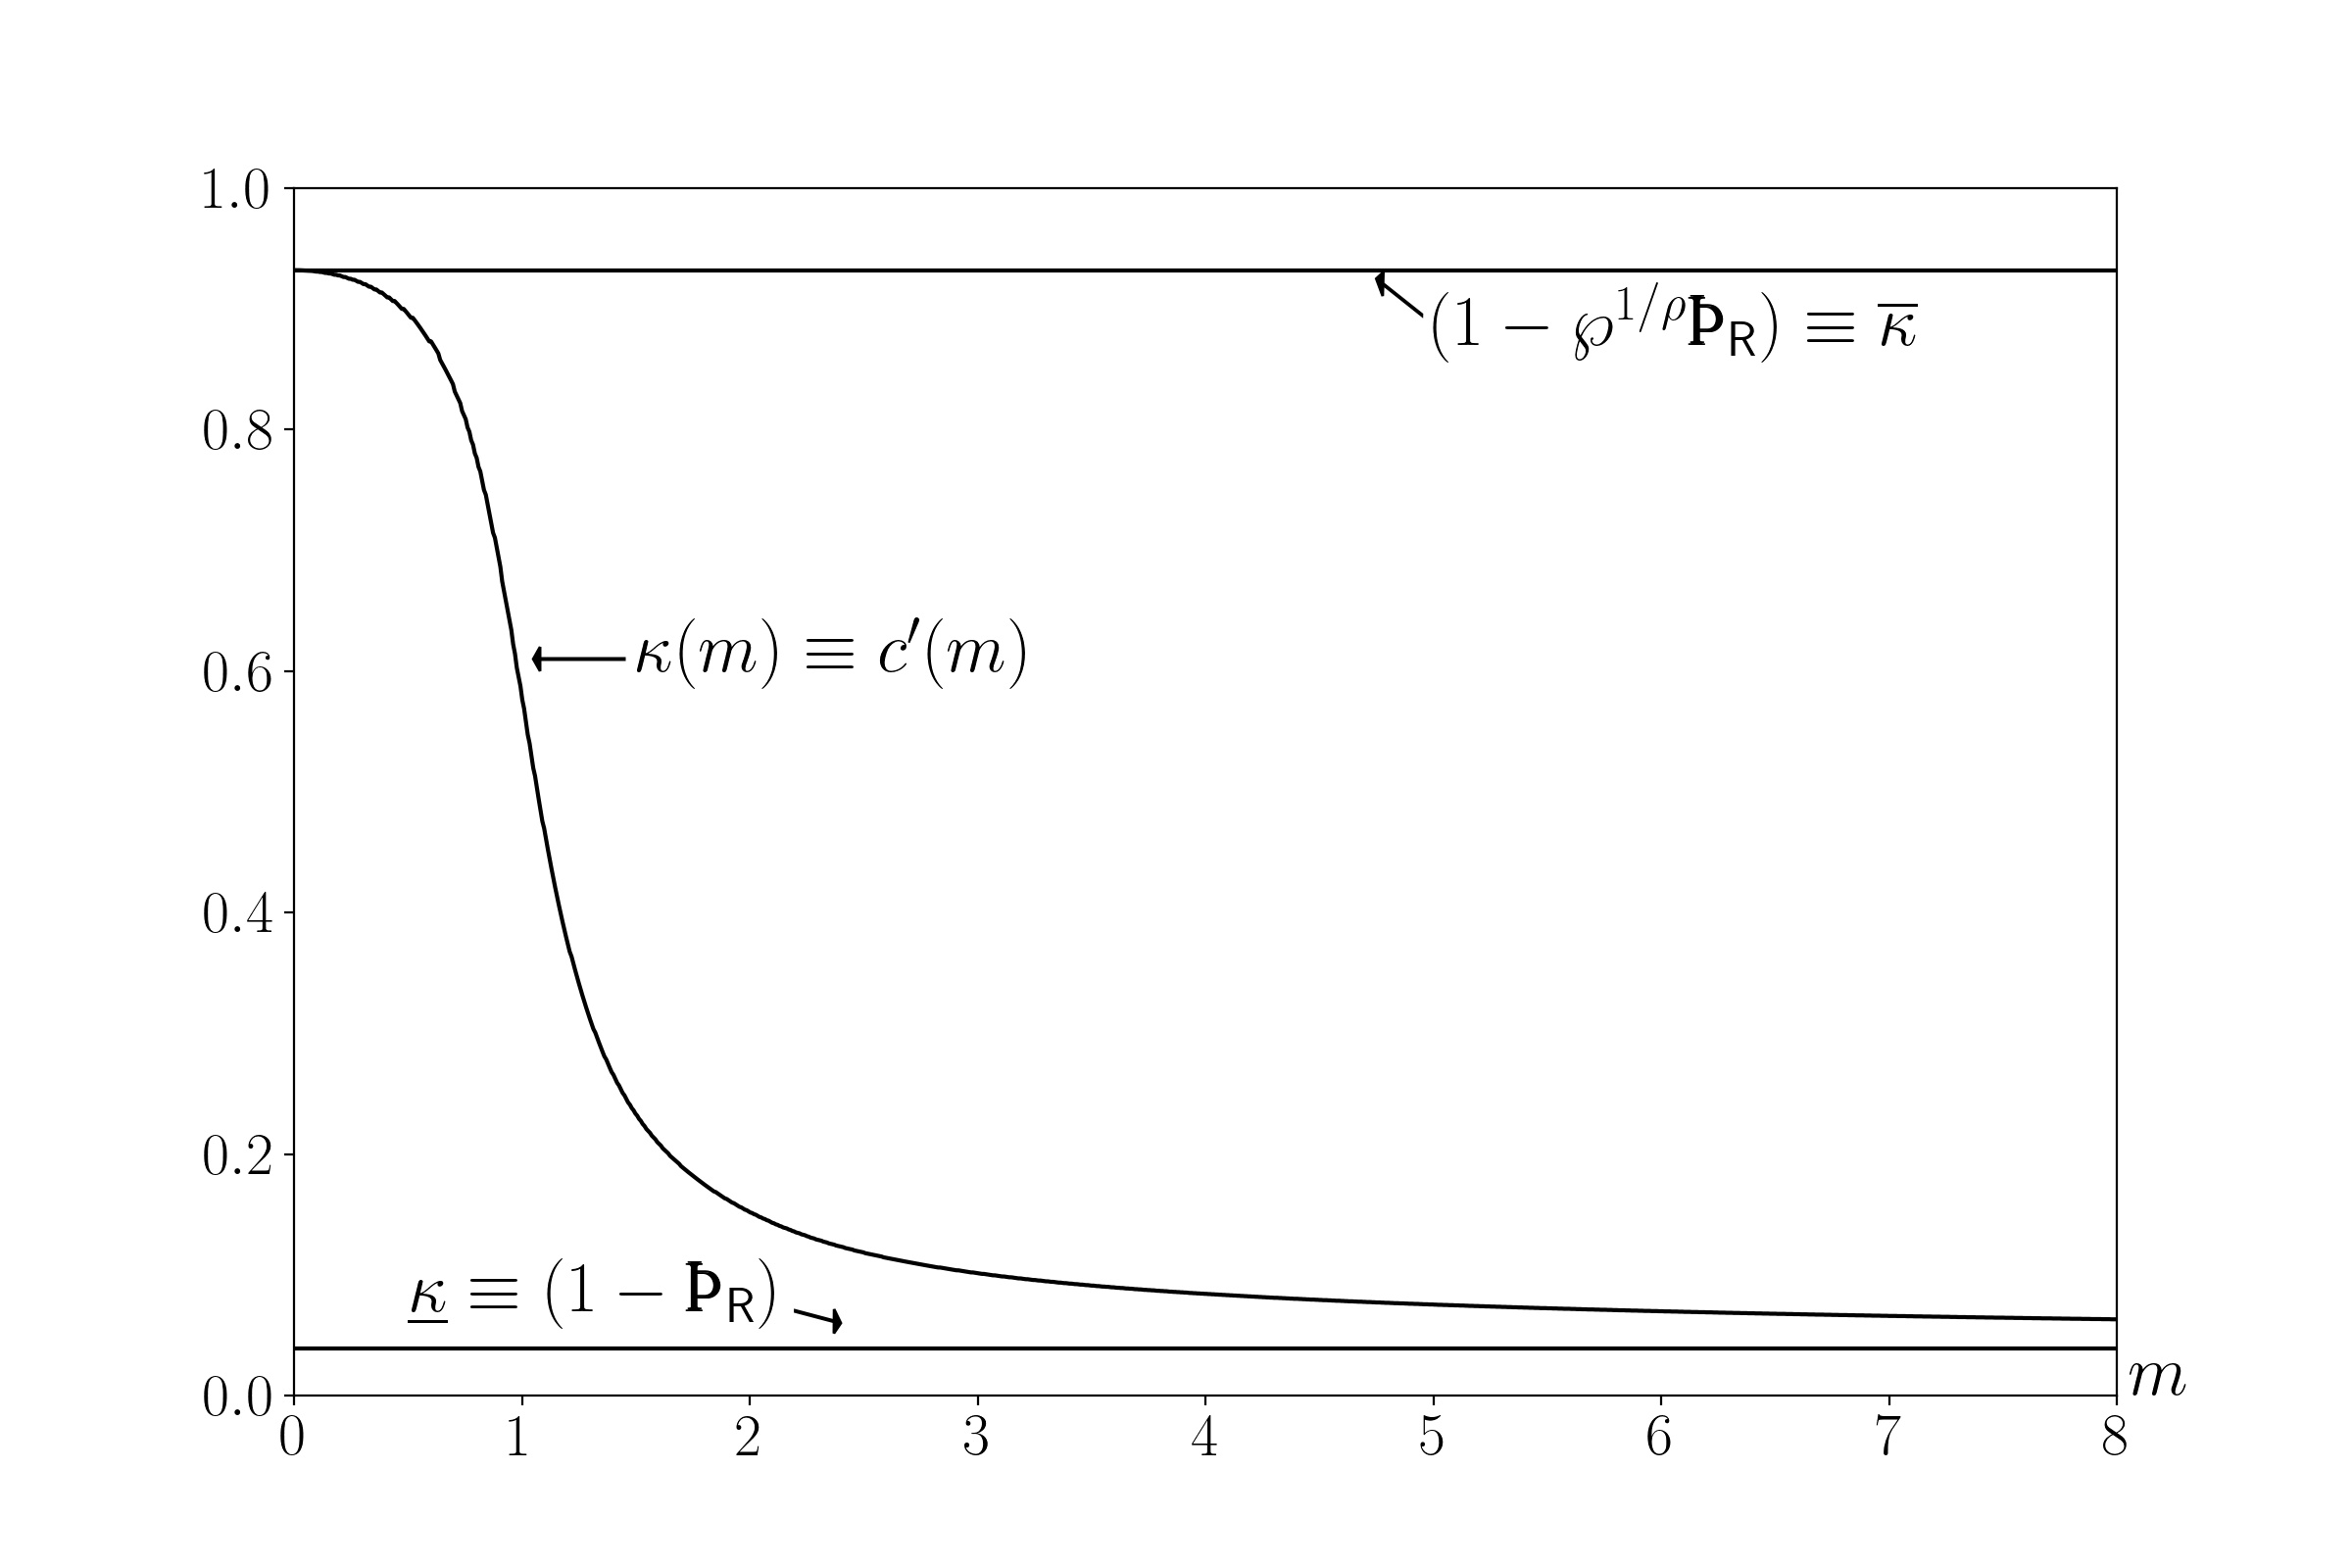
\includegraphics[width=0.8\linewidth]{\FigDir/MPCLimits}}  % Web 
\caption{Limiting MPC's} % Web 
\label{fig:mpclimits} % Web
\end{figure} % Web
}{ % Web - no
\begin{figure}
\centerline{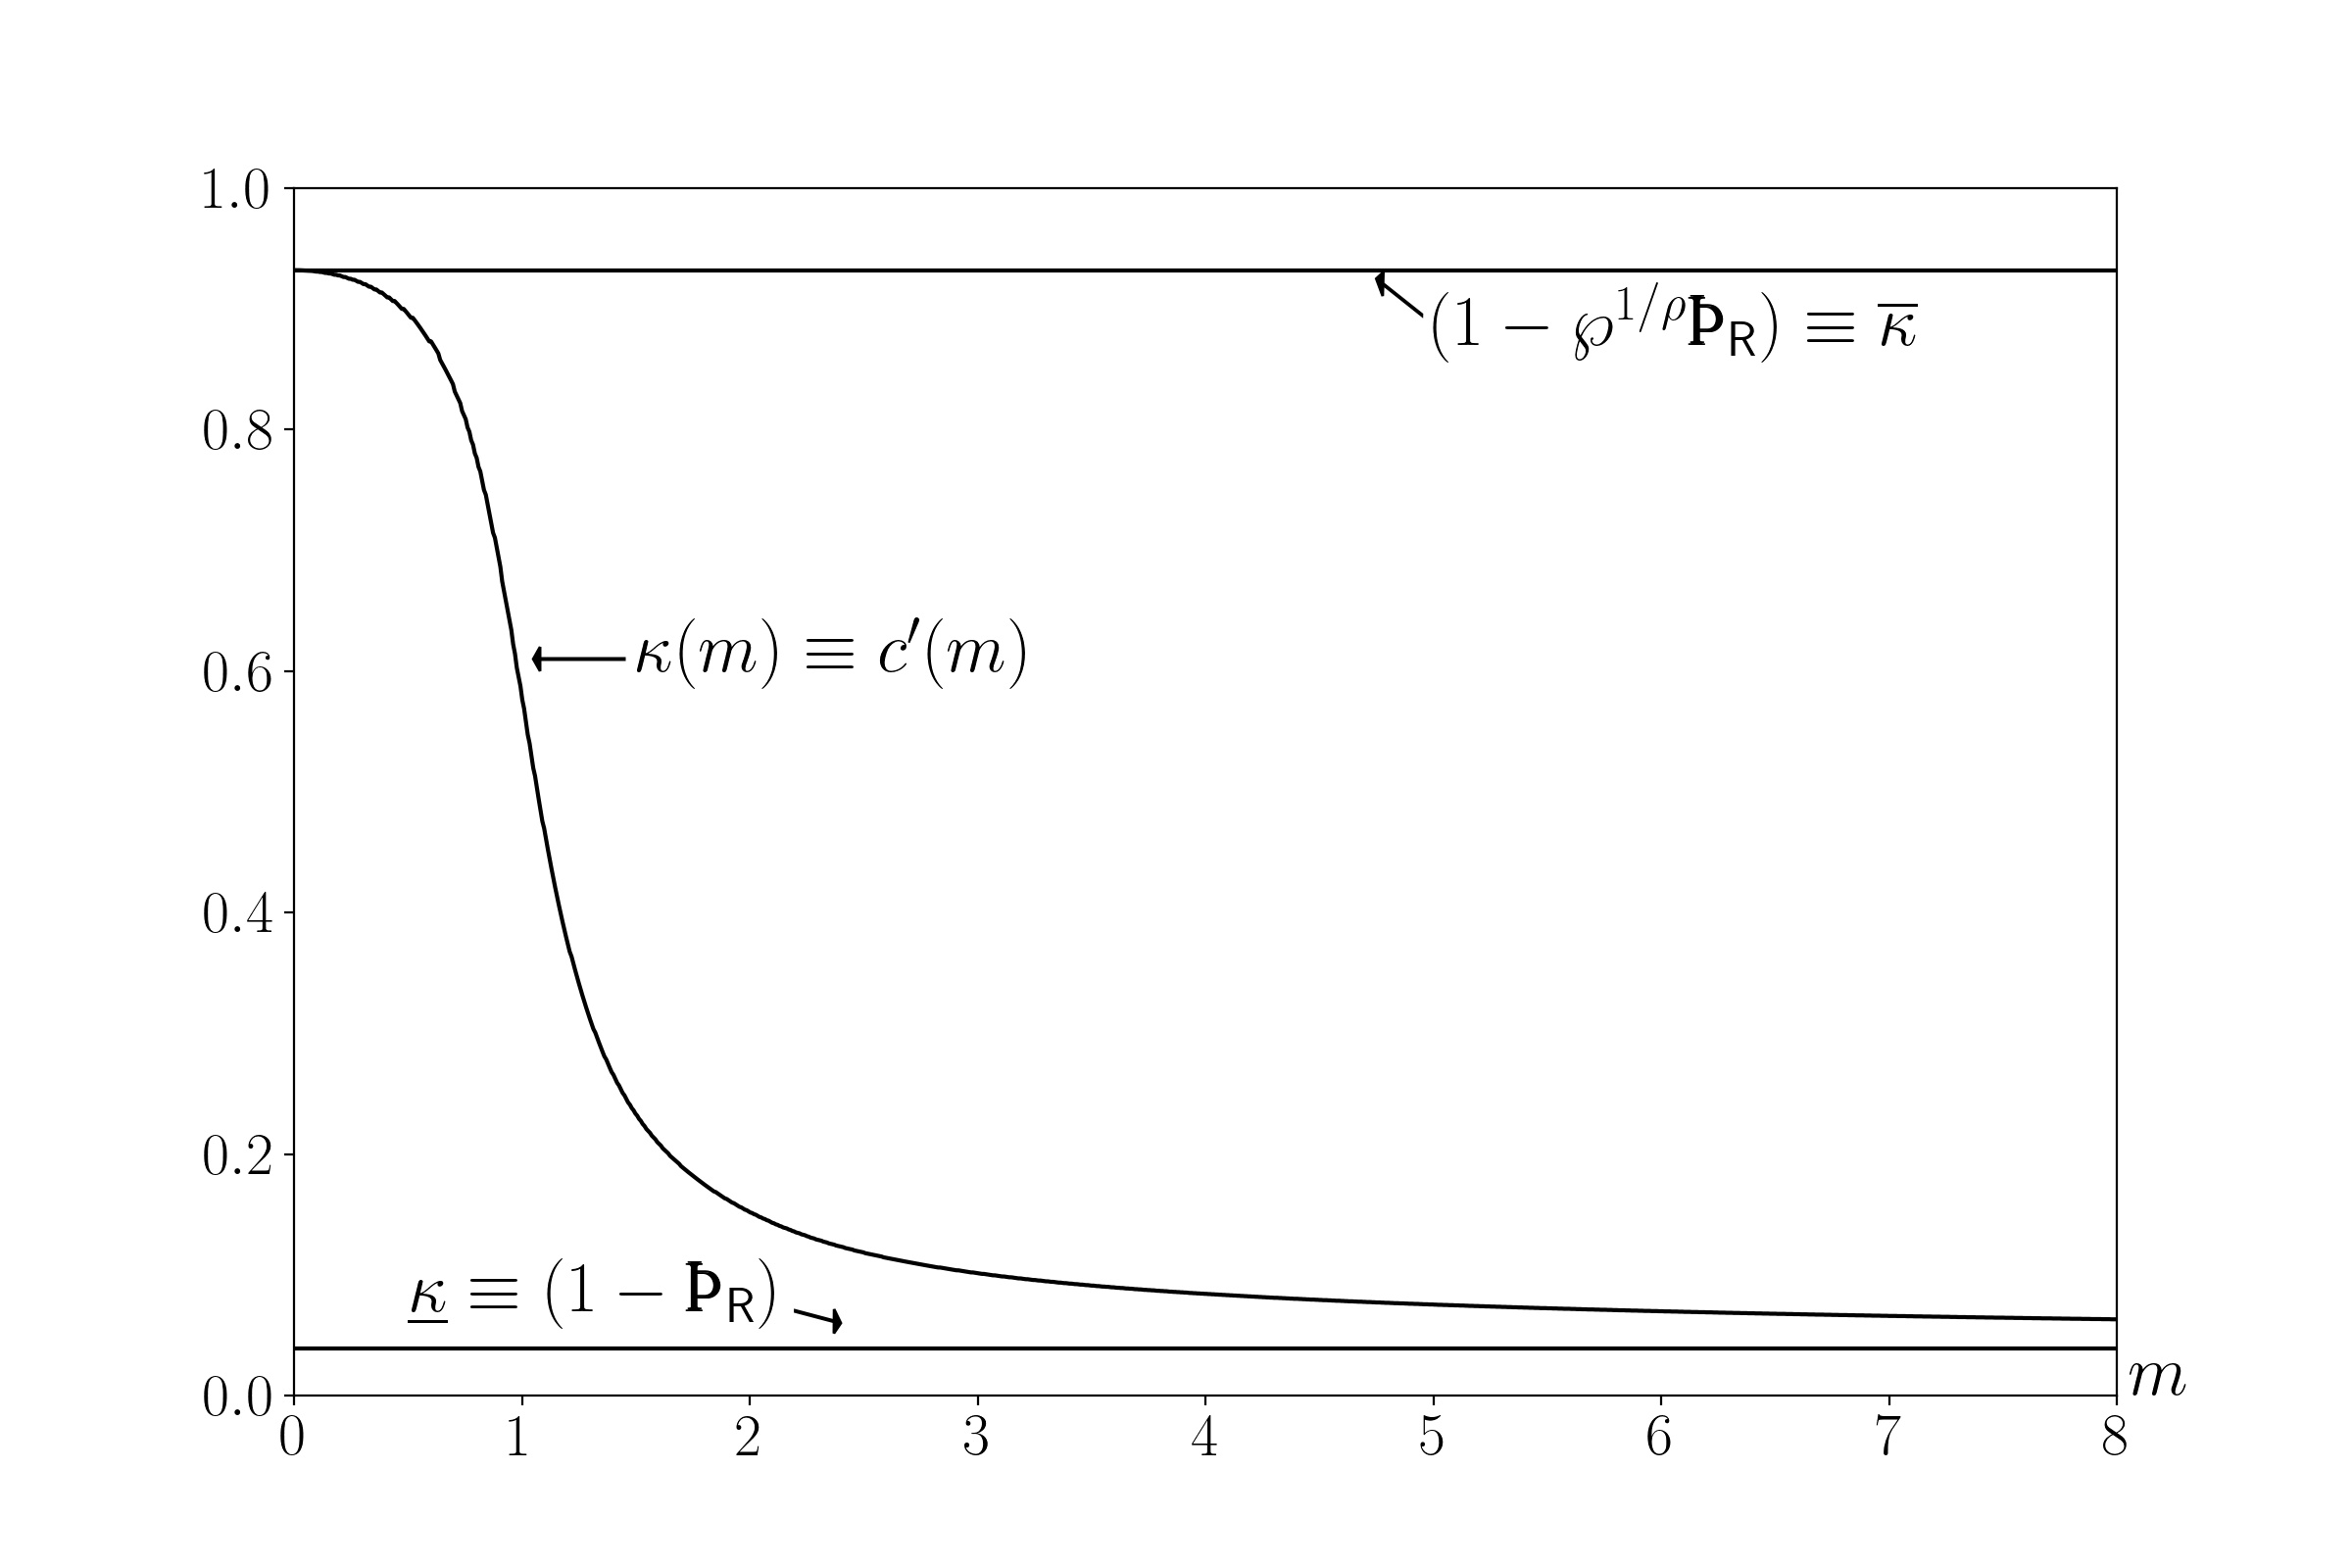
\includegraphics[width=6in]{\FigDir/MPCLimits}}
\caption{Limiting MPC's}
\label{fig:mpclimits}
\end{figure}
} % Web - no

\renewcommand{\figFile}{cFuncBounds}
\hypertarget{\figFile}{}
 \ifthenelse{\boolean{Web}}{
\begin{figure} % Web  
\centering % Web 
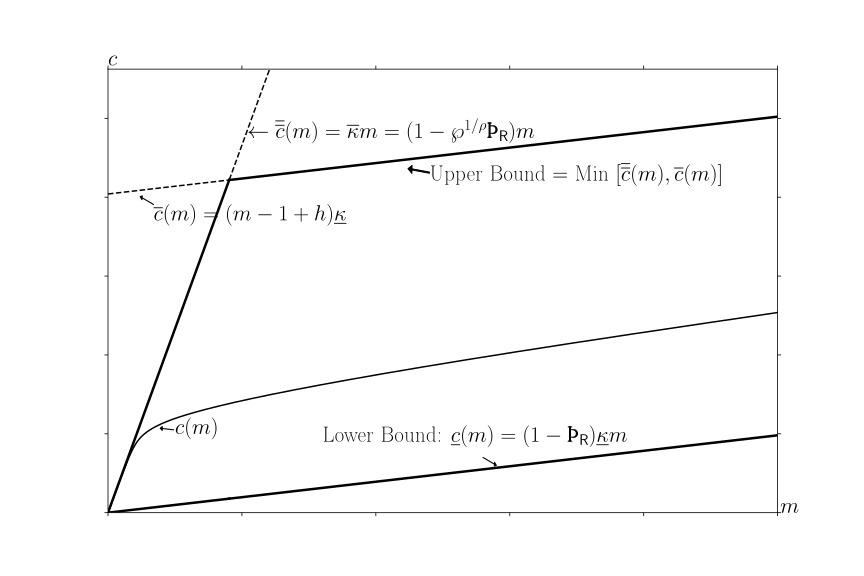
\includegraphics[width=0.7\linewidth]{\FigDir/cFuncBounds} % Web  
\caption{Upper and Lower Bounds on the Consumption Function} % Web  
\label{fig:cFuncBounds} % Web  
\end{figure} % Web  
}{ % Web  - no
\begin{figure}
\centering
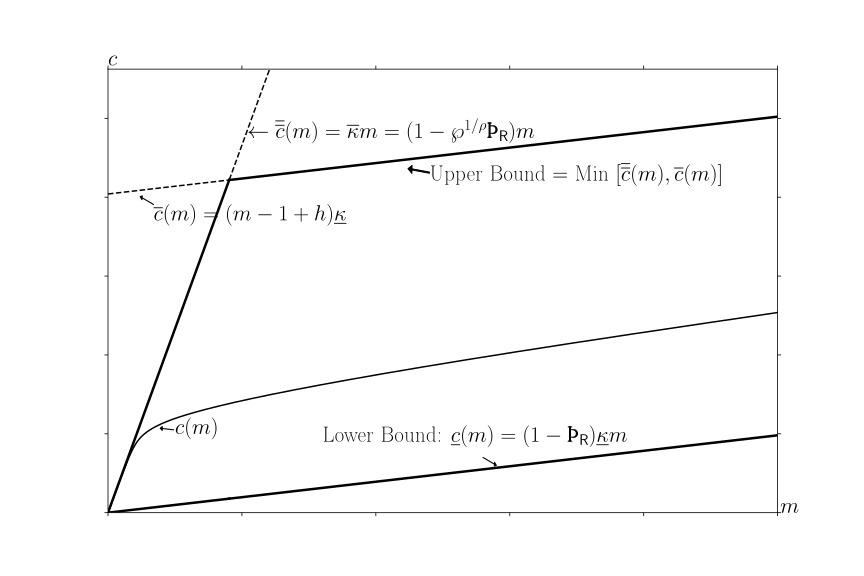
\includegraphics[width=6in]{\FigDir/cFuncBounds}
\caption{Upper and Lower Bounds on the Consumption Function}
\label{fig:cFuncBounds}
\end{figure}
}   % Web  -no


While in the presence of a constraint neither \hyperlink{RIC}{return impatience} nor \hyperlink{GIC}{growth impatience} is individually necessary for nondegeneracy of $\cFunc(m)$, a key conclusion of this section is that if \emph{both} \hyperlink{RIC}{return impatience} and \hyperlink{GIC}{growth impatience} fail, the consumption function \emph{will} be degenerate (limiting either to $\cFunc(m)=0$ or $c(\mNrm)=\infty$ as the horizon recedes).
So, for a useful solution, at least one of these conditions must hold.\footnote{Recall Claim \ref{claim:noRICGIC} showing that a double-impatience failure implies autarky value is not finite; and see } The case with \hyperlink{GIC}{growth impatience} but \hyperlink{RIC}{return \emph{patience}} is particularly surprising, because it is not immediately clear what prevents our earlier conclusion (in other circumstances) that return patience leads $\cFunc(m)$ to asymptote to zero.
The trick is to note that if return patience holds, $\Rfree < \APFac$, while failure of growth impatience means $\APFac < \PermGroFac$; together these inequalities tell us that $\Rfree < \PermGroFac$ so (limiting) human wealth is infinite.\footnote{This logic holds even if both $\Rfree$ and $\PermGroFac$ are less than one -- in this case, because the agent can \emph{borrow} at a negative interest rate and always repay with income that shrinks more slowly than their debt.}
But, if at any $\mNrm$ human wealth is unbounded, what prevents $\cFunc$ from asymptoting to $\cFunc(m)=\infty$ as the horizon gets arbitrarily long?
This is where the natural borrowing constraint comes in.
We will show that \hyperlink{GIC}{growth impatience} is sufficient, at any fixed $\mNrm$, to guarantee an upper bound to $\cFunc(m)$.
The insight is best understood by first abstracting from uncertainty and studying the perfect foresight case (with and without constraints).

\subsection{Model with Perfect Foresight}\label{subsec:PFBdiscussion}

\begin{comment}
Should we define the unconstrained problem?
\end{comment}

\hypertarget{ValuePFAnalytical}{}
\hypertarget{Autarky-Value-PF}{}

%\footnote{This is related to the key impatience condition in~\cite{asHomogeneous}.} % chktex 13<-- how(akshay)$

Claims \ref{claim:noRICGIC}-\ref{claim:PFConspC} established the relationship between the \hyperlink{PFFVAC}{finite value of autarky}, \hyperlink{RIC}{return impatience} and \hyperlink{GIC}{growth impatience} in the context of a model with uncertainty.
The easiest way to grasp the relations among these conditions is by studying Figure~\ref{fig:RelatePFGICFHWCRICPFFVAC}.
Each node represents a quantity defined above.
The arrow associated with each inequality imposes the condition, which is defined by the originating quantity being smaller than the arriving quantity.
For example, one way we wrote the \hypertarget{PFFVAC}{finite value of autarky} (under perfect foresight) in Equation~\eqref{eq:PFFVAC} is $\APFac < \Rfree^{1/\CRRA} \PermGroFac^{1-1/\CRRA}$, so imposition of \hypertarget{PFFVAC}{finite value of autarky} is captured by the diagonal arrow connecting $\APFac$ and $\Rfree^{1/\CRRA}\PermGroFac^{1-1/\CRRA}$.
Traversing the boundary of the diagram clockwise starting at $\APFac$ involves imposing first \hyperlink{GIC}{growth impatience} ($\APFac < \PermGroFac$) then \hypertarget{FHWC}{finite human wealth} ($\PermGroFac < \PermGroFac(\Rfree/\PermGroFac)^{1/\CRRA} \longleftrightarrow \PermGroFac < \Rfree $), and the consequent arrival at the bottom right node tells us that these two conditions jointly imply \hypertarget{PFFVAC}{perfect-foresight-finite-value-of-autarky}.
Reversal of a condition reverses the arrow's direction; so, for example, the bottom-most arrow going rightwards to $\Rfree^{1/\CRRA}\PermGroFac^{1-1/\CRRA}$ implies  \hypertarget{FHWC}{finite human wealth} fails; but we can cancel the cancellation and reverse the arrow.
This would allow us to traverse the diagram clockwise from $\APFac$  through $\PermGroFac$ to $\Rfree^{1/\CRRA}\PermGroFac^{1-1/\CRRA}$ to $\Rfree$, revealing that imposition of \hyperlink{GIC}{growth impatience} and \hypertarget{FHWC}{finite human wealth} (and, redundantly, \hypertarget{FHWC}{finite human wealth} again) let us conclude that \hyperlink{RIC}{return impatience} holds because the starting point is $\APFac$ and the endpoint is $\Rfree$ (and we have traversed a chain of `is greater than' relations).\footnote{Consult Appendix~\ref{sec:ApndxConditionDiagrams} for an exposition of diagrams of this type, which are a simple application of Category Theory~(\cite{riehl2017category}).}

% \figName allows generic definition of hypertargets based on title of figure
\renewcommand{\figName}{RelatePFGICFHWCRICPFFVAC} 
\hypertarget{\figName}{}
\input{Figures/\figName} % Read in the tex to generate the figure

In the unconstrained case, \hyperlink{FHWC}{finite human wealth} was necessary since, without constraints, only  this condition could prevent infinite borrowing in the limit (Proposition \ref{prop:pfUCFHWC}).
Looking at Figure~\ref{fig:RelatePFGICFHWCRICPFFVAC}, following the diagonal from $\APFac$ to the bottom-right corner corresponds to the direct of imposition of the \hyperlink{PFFVAC}{finite value of autarky}, which implies that the existence of a non-degenerate solution \textit{requires} \hyperlink{RIC}{return impatience} to hold.
To see why, if \hyperlink{RIC}{return impatience} failed, proceeding clockwise from the bottom left node of $\Rfree$ would lead to $\Rfree> \Rfree^{1/\CRRA}\PermGroFac^{1-1/\CRRA}$, (equivalently $(\PermGroFac/\Rfree)^{1-{1/\CRRA}}<1$) which corresponds to failure of \hyperlink{FHWC}{finite human wealth} (see also Case 3 in Section \ref{subsubsec:casesUC}).


We can understand how failure of \hyperlink{FHWC}{finite human wealth} leads to infinite borrowing thinking about \hyperlink{GIC}{growth impatience}.
From Figure~\ref{fig:RelatePFGICFHWCRICPFFVAC}, let \hyperlink{PFFVAC}{finite value of autarky} hold (traverse the diagonal from $\APFac$)  and then reverse the downward arrow from $\PermGroFac$, signifying the failure of \hyperlink{FHWC}{finite human wealth}, so that as the horizon extends and income grows faster than the rate at which it is discounted, there is no upper bound to the present discounted value of future income (cf.\ Equation \eqref{eq:LiqConstrBinds}).
But the cancellation of \hyperlink{FHWC}{finite human wealth} also indirectly implies that \hyperlink{GIC}{growth impatience} holds $\APFac > \Rfree^{1/\CRRA}\PermGroFac^{1-\CRRA} > \PermGroFac$ which tells us that this is a consumer who wants to spend out of their human wealth.
And therefore, at any fixed level of market resources, there is no upper bound to how much the consumer would choose to borrow as the horizon recedes.


\begin{comment}
An argument similar to the discussion pertaining to Equation \eqref{eq:LiqConstrBinds}, \textit{any} arbitrarily low (negative) constraint on $\bNrm_{t}$ becomes relevant.
Relaxing any constraint becomes always preferred and since income is guaranteed to grow faster than the rate of return, the consumer can continue to borrow without violating the no-ponzi condition (Equation \eqref{eq:NoDebtAtDeath}).
\end{comment}

Thus, in the perfect foresight unconstrained model, \hyperlink{RIC}{return impatience} is the only condition at our disposal that can prevent consumption from limiting to zero as the terminal period recedes.
However, when we impose a liquidity constraint, the range of admissible parameters becomes more interesting.

\hypertarget{PF-Constrained-Solution}{}
\hypertarget{Constrained-Solution}{}
\subsubsection{Perfect Foresight Constrained Solution}\label{subsec:PFCon}

We now sketch the perfect foresight constrained solution and demonstrate that a solution can exist either under \hyperlink{RIC}{return impatience} or without \hyperlink{RIC}{return impatience} but with \hyperlink{GIC}{growth impatience} (Proposition \ref{prop:PFCExist}).
Our discussion proceeds by examining implications of possible configurations of the patience conditions.
(Tables~\ref{table:Comparison} and~\ref{table:Required} codify.)


\paragraph{Case 1: Growth impatience fails and return impatience holds.} If \hyperlink{GIC}{growth impatience} fails but \hyperlink{RIC}{return impatience} holds, Appendix~\ref{sec:ApndxLiqConstr} shows that, for some $\mNrm_{\#}$, with $0 < \mNrm_{\#} < 1$, an unconstrained consumer behaving according to the perfect foresight solution~\eqref{eq:cFuncPFUnc} would choose $\cNrm < \mNrm$ for all $\mNrm > \mNrm_{\#}$.
In this case the solution to the constrained consumer's problem is simple; for any $\mNrm \geq \mNrm_{\#}$ the constraint does not bind (and will never bind in the future).
For such $\mNrm$ the constrained consumption function is identical to the unconstrained one.
If the consumer were somehow\footnote{``Somehow'' because $\mNrm<1$ could only be obtained by entering the period with $\bNrm < 0$ which the constraint forbids.} to arrive at an $\mNrm_{\#}$ such that $\mNrm < \mNrm_{\#} < 1$ the constraint would bind and the consumer would consume $\cNrm=\mNrm$.
Using $\cnstr{\cFunc}$ for the perfect foresight consumption function in the presence of constraints  (and analogously for all other functions):
\begin{equation*}
  \cnstr{\cFunc}(\mNrm)=
  \begin{cases}
    \mNrm & \text{if $\mNrm < \mNrm_{\#}$} \\
    \bar{\cFunc}(\mNrm)  & \text{if $\mNrm \geq \mNrm_{\#}$}
  \end{cases}
\end{equation*}
where $\bar{\cFunc}(\mNrm)$ is the unconstrained perfect foresight solution.


\paragraph{Case 2: Growth impatience holds and return impatience holds.}
When  \hyperlink{RIC}{return impatience} and  \hyperlink{GIC}{growth impatience} both hold, Appendix~\ref{sec:ApndxLiqConstr} shows that the limiting constrained consumption function is piecewise linear, with $\cnstr{\cFunc}(\mNrm)=\mNrm$ up to a first `kink point' at $\mNrm_{\#}^{0}>1$, and with discrete declines in the MPC at a set of kink points $\{\mNrm_{\#}^{1},\mNrm_{\#}^{2},\ldots\}$.
As $\mNrm \rightarrow \infty$ the constrained consumption function $\cnstr{\cFunc}(\mNrm)$ becomes arbitrarily close to the unconstrained $\bar{\cFunc}(\mNrm)$, and the marginal propensity to consume, $\cnstr{\cFunc}^{\prime}(\mNrm)$, limits to $\MPCmin$.\footnote{See~\cite{chkLiqConstr} for details.}
Similarly, the value function $\cnstr{\vFunc}(\mNrm)$ is non-degenerate and limits to the value function of the unconstrained consumer.


This logic holds even when \hyperlink{FHWC}{finite human wealth fails}, because the constraint prevents the (limiting) consumer\footnote{That is, one obeying $\cFunc(\mNrm) = \lim\limits_{n \rightarrow \infty} \cFunc_{t-n}(\mNrm)$.} from borrowing against unbounded human wealth to finance unbounded current consumption.
Under these circumstances, the consumer who starts with any $\bNrm_{t} > 0$ will, over time, run those resources down so that after some finite number of periods $\tau$ the consumer will reach $\bNrm_{t+\tau} = 0$, and thereafter will set $\cLvl = \permLvl$ for eternity (which \hypertarget{PFFVAC}{finite value of autarky} says yields finite value).
Using the same steps as for Equation~\eqref{eq:ValuePFAnalyticalAutarky}, value of the interim program is also finite: \hypertarget{PFFVAC}{}
\begin{align*}
  \vLvl_{t+\tau} 
  & = \PermGroFac^{\tau(1-\CRRA)} \uFunc(\permLvl_{t})\left(\frac{1-{(\DiscFac \PermGroFac^{1-\CRRA})}^{T-(t+\tau)+1}}{1-\DiscFac \PermGroFac^{1-\CRRA}}\right).
\end{align*}
% Note that the last version of the \PFFVAC~in~\eqref{eq:PFFVAC} implies the \GICRaw~$\GPFacRaw < 1$ whenever \cncl{\FHWC} ($\Rfree < \PermGroFac$) holds.
So, even when \hyperlink{FHWC}{finite human wealth fails}, the limiting consumer's value for any finite $\mNrm$ will be the sum of two finite numbers: One due to the unconstrained choice made over the finite-horizon leading up to $\bNrm_{t+\tau} = 0$, and one reflecting the value of consuming $\permLvl_{t+\tau}$ thereafter.

\hypertarget{RICandFHWCFail}{}
\paragraph{Case 3: Growth impatience holds and return impatience fails.} The most peculiar possibility occurs only when \hyperlink{RIC}{return impatience} fails.
As noted above, this possibility is unavailable to us without a constraint.
Without return impatience, \hyperlink{FHWC}{finite human wealth} must also fail (Appendix~\ref{sec:ApndxLiqConstr}), and the constrained consumption function is (surprisingly) non-degenerate.
(See appendix Figure~\ref{fig:PFGICHoldsFHWCFailsRICFails} for a numerical example).
Even though human wealth is unbounded at any given level of $\mNrm$, since borrowing is ruled out, consumption cannot become unbounded at that $\mNrm$ in the limit as the horizon recedes.
However, the failure of return impatience does have some power: It means that as $\mNrm$ rises without bound, the MPC approaches zero ( $\lim\limits_{m \rightarrow \infty} \cnstr{\cFunc}^{\prime}(\mNrm) = 0$).
Nevertheless $\cnstr{\cFunc}(\mNrm)$ is finite, strictly positive, and strictly increasing in $\mNrm$.
This result reconciles the conflicting intuitions from the unconstrained case, where failure of \hyperlink{RIC}{return impatience} would suggest a degenerate limit of $\cnstr{\cFunc}(\mNrm)=0$ while failure of \hyperlink{FHWC}{finite human wealth} would suggest a degenerate limit of $\cnstr{\cFunc}(\mNrm)=\infty$.





\hypertarget{model-with-uncertainty}{}
\subsection{Model with Uncertainty}\label{subsec:TheModelUncertainty}

We now examine the case with uncertainty but without constraints, which we argued was a close parallel to the model with constraints but without uncertainty (recall Section \ref{subsubsec:deatonIsLimit}).
\hypertarget{Calibration}{}
\newlength\TableWidth
\newsavebox{\Parameters}
\begin{table}
  \centering
\renewcommand{\arraystretch}{1.2}
  \caption{Microeconomic Model Calibration}\label{table:Parameters}
\sbox{\Parameters}{
\begin{tabular}{|c|ccl|c|}
\hline
\multicolumn{5}{|l|}{Calibrated Parameters}  \\ \hline
Description                     & \multicolumn{1}{c}{Parameter} & Value & \multicolumn{2}{c|}{Source}\\ \hline
Permanent Income Growth Factor  & \multicolumn{1}{c}{$\PermGroFac$} & 1.03 & \multicolumn{2}{c|}{PSID: Carroll (1992)} \\
Interest Factor                 & \multicolumn{1}{c}{$\Rfree$} & 1.04 & \multicolumn{2}{c|}{Conventional} \\
Time Preference Factor          & \multicolumn{1}{c}{$\beta$} & 0.96 & \multicolumn{2}{c|}{Conventional} \\
Coefficient of Relative Risk Aversion & \multicolumn{1}{c}{$\CRRA$} & 2 & \multicolumn{2}{c|}{Conventional} \\
Probability of Zero Income      & \multicolumn{1}{c}{$\pZero$} & 0.005 & \multicolumn{2}{c|}{PSID: Carroll (1992)} \\
Std Dev of Log Permanent Shock  & \multicolumn{1}{c}{$\sigma_{\PermShk}$} & 0.1 & \multicolumn{2}{c|}{PSID: Carroll (1992)} \\
Std Dev of Log Transitory Shock & \multicolumn{1}{c}{$\sigma_{\theta}$} & 0.1 & \multicolumn{2}{c|}{PSID: Carroll (1992)} \\ \hline
\end{tabular}
} % End \sbox

\settowidth\TableWidth{\usebox{\Parameters}}
\usebox{\Parameters}
\end{table}


\hypertarget{Symbols}{}

  \begin{table}
    \centering
    \renewcommand{\arraystretch}{1.3}
    \caption{Model Characteristics Calculated from Parameters}\label{table:Calibration}
    \sbox{\TblBox}{
      \begin{tabular}{|c|ccl|c|}
        \hline
        % \multicolumn{5}{|l|}{Model Characteristics Calculated From Parameters}  \\ \hline
        & \multicolumn{3}{c|}{}                                      & Approximate \\
        & \multicolumn{3}{c|}{}                                       & Calculated \\
        Description                                 & \multicolumn{3}{c|}{Symbol and Formula}                       & Value \\ \hline
        \hyperlink{FHWFacDefn}{Finite Human Wealth Factor}                 & $\RNrmByGRnd^{-1}$ & $\equiv$ & $\PermGroFac/\Rfree$                    & 0.990 \\
        \hyperlink{VAFacDefn}{PF Value of Autarky Factor} & $\beth$ & $\equiv$ & $\DiscFac \PermGroFac^{1-\CRRA}$                    & 0.932 \\
        \hyperlink{InvEPermShkEInv}{Growth Compensated Permanent Shock}            & $\InvEPermShkInv $ & $\equiv$ & $ (\EPermShkInv)^{-1}$               & 0.990 \\
        \hyperlink{PermGroFacAdj}{Uncertainty-Adjusted Growth}                 & $\PermGroFacAdj $ & $\equiv$ & $ \PermGroFac \InvEPermShkInv$        & 1.020 \\
        \hyperlink{uInvEuPermShk}{Utility Compensated Permanent Shock}                & $\uInvEuPermShk $ & $\equiv$ & $ (\Ex[\permShk^{1-\CRRA}])^{1/(1-\CRRA)}$ & 0.990 \\
        \hyperlink{PermGroFacAdj}{Utility Compensated Growth}                     & $\PermGroFacAdj $ & $\equiv$ & $ \PermGroFac \uInvEuPermShk$        & 1.020 \\
        \hyperlink{APFacDefn}{Absolute Patience Factor}                    & $\APFac_{\phantom{\Rfree}} $ & $\equiv$ & $ (\Rfree \DiscFac)^{1/\CRRA}$                & 0.999 \\
        \hyperlink{RPFacDefn}{Return Patience Factor}                      & $\RPFac$ & $\equiv$ & $\APFac/\Rfree $     & 0.961 \\
        \hyperlink{GPFacRawDefn}{\phantom{Modified }Growth Patience Factor}    & $\GPFacRaw$ & $\equiv$ & $\APFac/\PermGroFac $      & 0.970 \\
        \hyperlink{GPFacRawDefn}{Modified Growth Patience Factor}                      & $\GPFacMod$ & $\equiv$ & $ \APFac/\PermGroFacAdj$& 0.980 \\
        \hyperlink{VAFacDefn}{Value of Autarky Factor}         & $\DiscAltuAdj $ & $\equiv$ & $ \DiscFac \PermGroFac^{1-\CRRA}\uInvEuPermShk^{1-\CRRA}$       & 0.941 \\
        \hyperlink{WRIC}{Weak Return Impatience Factor}         & $\pZero^{1/\CRRA} \APFac $ & $\equiv$ & $ (\pZero \DiscFac \Rfree)^{1/\CRRA}$       & 0.071 \\ \hline
      \end{tabular}
    } % End \sbox

    \settowidth\TableWidth{\usebox{\TblBox}}
    \savebox{\TblShrunkBox}{
      \settowidth{\TblShrunk}{\usebox{\TblBox}}
      \resizebox{0.9\textwidth}{!}{\begin{minipage}{\TblShrunk}
          \usebox{\TblBox}
        \end{minipage}}
    }

    \usebox{\TblShrunkBox}


%    \parbox{\textwidth}{\footnotesize The \href{https://econ-ark.org/materials/bufferstocktheory-dashboard?launch}{dashboard} permits experimentation with alternative parameter values.}
  \end{table}


%\hypertarget{Relations-Between-Parametric-Restrictions}{}
%\subsubsection{Relations Between Parametric Restrictions}

Tables~\ref{table:Parameters} and~\ref{table:Calibration} present calibrations and values of model conditions in the case with uncertainty, where \hyperlink{RIC}{return impatience}, \hyperlink{GICRaw}{growth impatience} and \hyperlink{FVAC}{finite value of autarky} all hold.
The full relationship among conditions is represented in Figure~\ref{fig:Inequalities}.
Though the diagram looks complex, it is merely a modified version of the earlier simple diagram (Figure~\ref{fig:RelatePFGICFHWCRICPFFVAC}) with further (mostly intermediate) inequalities inserted.
(Arrows with a ``because'' now label relations that always hold under the model's assumptions.)\footnote{Again, readers unfamiliar with such diagrams should see Appendix~\ref{sec:ApndxConditionDiagrams} for a more detailed exposition.}

\renewcommand{\figName}{Inequalities} 
\renewcommand{\figFile}{\figName} 
\hypertarget{\figFile}{}
\input{Figures/\figName} % Read in the tex to generate the figure

Beyond \hyperlink{FVAC}{finite value of autarky},
the additional condition sufficient for contraction, \hyperlink{WRIC}{weak return impatience}, can be seen to be weak by asking `under what circumstances would the \hyperlink{FVAC}{finite value of autarky} hold but the \hyperlink{WRIC}{weak return impatience} fail?'  Algebraically, the requirement becomes:
%
\begin{align}
  \DiscFac \PermGroFac^{1-\CRRA}\uInvEuPermShk^{1-\CRRA} & < ~ 1 ~ <  {(\pZero \DiscFac)}^{1/\CRRA}/\Rfree^{1-1/\CRRA}. \label{eq:WRICandFVAC}
\end{align}
%
where $\uInvEuPermShk \colon = (\Ex[\permShk^{1-\CRRA}])^{1/(1-\CRRA)} < 1$.
If we require $\Rfree \geq 1$, the \hyperlink{WRIC}{weak return impatience} is `redundant' because now $\DiscFac <1<\Rfree^{\CRRA-1}$, so that (with $\CRRA > 1$ and $\DiscFac<1$) \hyperlink{RIC}{return impatience} (and \hyperlink{WRIC}{weak return impatience}) must hold.
But neither theory nor evidence demand that $\Rfree \geq 1$.
We can therefore approach the question of the relevance of \hyperlink{WRIC}{weak return impatience}  by asking just how low $\Rfree$ must be for the condition to be relevant.
Suppose for illustration that $\CRRA=2$, $\uInvEuPermShk^{1-\CRRA}=1.01$, $\PermGroFac^{1-\CRRA}=1.01^{-1}$ and $\pZero = 0.10$.
In that case~\eqref{eq:WRICandFVAC} reduces to:
\begin{align*}
  \DiscFac  & < 1 < {(0.1 \DiscFac/\Rfree)}^{1/2},
\end{align*}
but since $\DiscFac < 1$ by assumption, the binding requirement becomes:
\begin{align*}
  \Rfree  & < \DiscFac/10, \notag
\end{align*}
so that for example if $\DiscFac=0.96$ we would need $\Rfree < 0.096$ (that is, a perpetual riskfree rate of return of worse than -90 percent a year) in order for \hyperlink{WRIC}{weak return impatience} to be nonredundant.


Perhaps the best way of thinking about this is to note that the space of parameter values for which the \hyperlink{WRIC}{weak return impatience}  remains relevant shrinks out of existence as $\pZero \rightarrow 0$, which Section~\ref{subsubsec:deatonIsLimit} showed was the precise limiting condition under which behavior becomes arbitrarily close to the liquidity constrained solution (in the absence of other risks).
On the other hand, when $\pZero = 1$, the consumer has no noncapital income (so \hyperlink{FHWC}{finite human wealth} holds) and with $\pZero=1$ \hyperlink{WRIC}{weak return impatience} is identical to \hyperlink{WRIC}{weak return impatience}.
However, \hyperlink{WRIC}{weak return impatience} is the only condition required for a solution to exist for a perfect foresight consumer with no noncapital income.
Thus \hyperlink{WRIC}{weak return impatience} forms a sort of `bridge' between the liquidity constrained and the unconstrained problems as $\pZero$ moves from 0 to 1.

\subsubsection{Behavior Under Cases of Conditions}\label{subsubsec:casesUC}

\hypertarget{IntuitionRIC}{}
%\subsubsection{When the {RIC}~Fails}\label{subsubsec:WhenTheRICFails}
\paragraph{Case 1: Return impatience fails and growth impatience holds} 

In the unconstrained perfect foresight problem (Section~\ref{subsec:PFBbenchmark}), \hyperlink{RIC}{return impatience} was necessary for existence of a non-degenerate solution.
It is surprising, therefore, that in the presence of uncertainty, the much weaker \hyperlink{WRIC}{weak return impatience} is sufficient for nondegeneracy (assuming that \hyperlink{FVAC}{finite value of autarky}  holds).
Given \hyperlink{FVAC}{finite value of autarky}, we can derive the features the problem must exhibit for \hyperlink{RIC}{return impatience} to fail (that is, $\Rfree < {(\Rfree \DiscFac)}^{1/\CRRA}$) (given that growth impatience holds) as follows:
%
\begin{equation}\label{eq:RICimplies}
  \begin{split}
    \Rfree   & < {(\Rfree \DiscFac)}^{1/\CRRA} ~ < ~ {(\Rfree {(\PermGroFac \uInvEuPermShk)}^{\CRRA-1})}^{1/\CRRA}
    \\ \Rightarrow \Rfree   & < {(\Rfree/\PermGroFac)}^{1/\CRRA}\PermGroFac \uInvEuPermShk^{1-1/\CRRA}
                   %         \\  \Rfree/\PermGroFac  & < {(\Rfree/\PermGroFac)}^{1/\CRRA}\uInvEuPermShk^{1-1/\CRRA}
    \\  \qquad\qquad\qquad \Rightarrow  \Rfree/\PermGroFac  & < \uInvEuPermShk
  \end{split}
\end{equation}
%
but since $\uInvEuPermShk < 1$ (for $\CRRA>1$ and non-degenerate $\permShk$), this requires $\Rfree/\PermGroFac < 1$.
Thus, given \hyperlink{FVAC}{finite value of autarky}, \hyperlink{RIC}{return impatience} can fail only if human wealth is unbounded and \hyperlink{GIC}{growth impatience} holds.\footnote{This algebraically complicated conclusion could be easily reached diagrammatically in Figure~\ref{fig:Inequalities} by starting at the $\Rfree$ node and imposing the failure of \hyperlink{RIC}{return impatience}, which reverses the \hyperlink{RIC}{return impatience} arrow and lets us traverse the diagram along any clockwise path to the \hyperlink{PFFVAC}{perfect foresight finite value of autarky} node at which point we realize that we \textit{cannot} impose \hyperlink{FHWC}{finite human wealth} because that would let us conclude $\Rfree > \Rfree$.}

As in the perfect foresight constrained problem, unbounded limiting human wealth here does not lead to a degenerate limiting consumption function (finite human wealth is not required for Theorem \ref{thm:convgtobellman}).
But, from equation~\eqref{eq:PFMPCminInv} and the discussion surrounding it, an implication of the failure of \hyperlink{RIC}{return impatience} is that $\lim\limits_{m \rightarrow \infty} \usual{\cFunc}^{\prime}(\mNrm) = 0$.
Thus, interestingly, in this case (unavailable in the perfect foresight unconstrained) model the presence of uncertainty both permits unlimited human wealth (in the $n\rightarrow\infty$ limit) and at the same time prevents unlimited human wealth from resulting in (limiting) infinite consumption (at any finite $\mNrm$).
Intuitively, the utility-imposed `natural constraint' that arises from the possibility of a zero income event prevents infinite borrowing and at the same time allows infinite human wealth to prevent patience from resulting, as it does under other conditions, in the degenerate $\usual{\cFunc}(\mNrm)=0$ as the terminal period recedes.
Thus, in presence of uncertainty of the kind we assume, pathological patience (which in the perfect foresight model results in a limiting consumption function of $\usual{\cFunc}(\mNrm)=0$) plus unbounded human wealth (which the perfect foresight model prohibits because it leads to a limiting consumption function $\usual{\cFunc}(\mNrm)=\infty$ for any finite $\mNrm$) combine to yield a unique finite limiting (as $n \rightarrow \infty$) level of consumption and MPC for any finite value of $\mNrm$.


Note the close parallel to the conclusion in the perfect foresight liquidity constrained model in the case where \hyperlink{RIC}{return impatience} fails (Case 3 in Section \ref{subsec:PFCon}).
There, too, the tension between infinite human wealth and pathological patience was resolved with a non-degenerate consumption function whose limiting MPC was zero.\footnote{\cite{maTodaRich} derive conditions under which the limiting MPC is zero in an even more general case where there is also capital income risk.}

\hypertarget{When-the-RIC-Holds}{}
%\subsubsection{When the {RIC} Holds}\label{subsubsec:WhenTheGICModFails}\label{subsubsec:WhenTheRICHolds}
\paragraph{Case 2: Return impatience holds and growth impatience holds with finite human wealth} 
This is the benchmark case we presented at the start of the Section.
If \hyperlink{RIC}{return impatience}  and \hyperlink{FHWC}{finite human wealth} both hold, a perfect foresight solution exists (Section \ref{subsec:PFBbenchmark}).
As $\mNrm \rightarrow \infty$ the limiting $\cFunc$ and $\vFunc$ functions become arbitrarily close to those in the perfect foresight model, because human wealth pays for a vanishingly small portion of spending (Section \ref{subsubsec:cFuncBounds}).

\paragraph{Case 3: Return impatience holds and growth impatience holds with infinite human wealth} The more exotic case is where \hyperlink{FHWC}{finite human wealth} fails but both \hyperlink{GIC}{growth impatience} and \hyperlink{RIC}{return impatience} also hold.
In the unconstrained perfect foresight model, this is the degenerate case with limiting $\bar{\cFunc}(\mNrm)=\infty$.
Here, \hyperlink{FHWC}{infinite human wealth} and \hyperlink{FVAC}{finite value of autarky} implies that \hyperlink{FVAC}{(perfect foresight) finite value of autarky} holds and that $ \APFac < \PermGroFac$.
To see why, traverse Figure~\ref{fig:Inequalities} clockwise from $\APFac$ by imposing \hyperlink{FVAC}{finite value of autarky} to reach the \hyperlink{PFFVAC}{PF-FVAF}  node.
Because the bottom arrow pointing to the right, connecting the $\Rfree$ and \hyperlink{PFFVAC}{perfect foresight finite value of autarky} nodes imposes the failure of finite human wealth (and here we are assuming that condition holds), we can reverse the bottom arrow and traverse the resulting clockwise path from {FVAC} to see that 
%
\begin{align*}
  & \APFac < {(\Rfree/\PermGroFac)}^{1/\CRRA}\PermGroFac \Rightarrow  \APFac < \PermGroFac
\end{align*}
%
where the transition from the first to the second lines is justified because failure of \hyperlink{FHWC}{finite human wealth} implies $\Rightarrow {(\Rfree/\PermGroFac)}^{1/\CRRA}<1$.
So, under \hyperlink{RIC}{return impatience} and \hyperlink{FHWC}{finite human wealth}, we must have \hyperlink{GIC}{growth impatience}.

However, we are not entitled to conclude that \hyperlink{GICMod}{strong growth impatience} holds: $\APFac < \PermGroFac$ does not imply $\APFac < \InvEPermShkInv \PermGroFac$ where $\InvEPermShkInv<1$.
 
 \begin{comment}
 (traverse Figure~\ref{fig:Inequalities} clockwise from $\APFac$ by imposing {\FVAC} and continue to the {\PFVAFacDefn} node):  Reversing the arrow connecting the $\Rfree$ and {\PFVAFacDefn} nodes implies that under $\cncl{\FHWC}$:
\begin{align*}
  & \overbrace{\APFac < {(\Rfree/\PermGroFac)}^{1/\CRRA}\PermGroFac}^{\PFFVAC}
  \\ & \APFac < \PermGroFac
\end{align*}
where the transition from the first to the second lines is justified because $\cncl{\FHWC} \Rightarrow {(\Rfree/\PermGroFac)}^{1/\CRRA}<1$.
So, \{\RIC, \cncl{\FHWC}\} implies the {\GICRaw} holds.

\end{comment}

We have now established the principal points of comparison between the perfect foresight solutions and the solutions under uncertainty; these are codified in the remaining parts of Tables~\ref{table:Comparison} and~\ref{table:Required}.

\hypertarget{Factors-Defined-And-Compared}{}
  \begin{table}[!th]
    \centering
\caption{Definitions and Comparisons of Conditions}
  \iflabelexists{table:Comparison}{}{\label{table:Comparison}} % Don't define it if already defined
  \sbox{\TblBox}{
\begin{tabular}{|c|c|}\hline
Perfect Foresight Versions & Uncertainty Versions\\ \hline
\multicolumn{2}{|c|}{Finite Human Wealth Condition (\FHWC)} \\ \hline
$\PermGroFac/\Rfree < 1$                                                          & $\PermGroFac/\Rfree < 1$ \\
\multirow{3}{75mm}{\thead{The growth factor for permanent income \\ $\PermGroFac$ must be smaller than the discounting \\ factor $\Rfree$ for human wealth to be finite. }} &
\multirow{3}{75mm}{\thead{The model's risks are mean-preserving \\ spreads, so the PDV of future income is \\ unchanged by their introduction.}} \\
&  \\
&  \\
&  \\ \hline
\multicolumn{2}{|c|}{Absolute Impatience Condition (\AIC)} \\ \hline
$\APFac < 1$                                        &  $\APFac < 1$ \\
\multirow{4}{75mm}{\thead{The unconstrained consumer is \\ sufficiently impatient that the level of \\ consumption will be declining over time:}} &
\multirow{4}{75mm}{\thead{\textit{If wealth is large enough,} the \textit{expectation} \\ of consumption next period will be \\ smaller than this period's consumption:}} \\
& \\
& \\
& \\
$\cLvl_{t+1} < \cLvl_{t}$ & $\displaystyle \lim_{m_{t} \rightarrow \infty} \Ex_{t} [\cLvl_{t+1}] < \cLvl_{t}$ \\
& \\ \hline
\multicolumn{2}{|c|}{Return Impatience Conditions} \\ \hline
\multicolumn{1}{|c|}{Return Impatience Condition (\RIC)} & \multicolumn{1}{c|}{Weak \RIC~(\WRIC)} \\ \hline
$\APFac/\Rfree < 1$                                          & $\pZero^{1/\CRRA}\APFac/\Rfree < 1$ \\
\multirow{3}{75mm}{\thead{The growth factor for consumption $\APFac$ \\ must be smaller than the discounting \\ factor $\Rfree$, so that the PDV of current and \\ future consumption will be finite:}}  &
\multirow{3}{75mm}{\thead{If the probability of the zero-income \\ event is $\pZero=1$ then income is always zero \\ and the condition becomes identical to \\ the \RIC.  Otherwise, weaker.}} \\
& \\
& \\
& \\
& \\
$\cFunc^{\prime}(m) = 1-\APFac/\Rfree < 1$              & $\cFunc^{\prime}(m) < 1-\pZero^{1/\CRRA}\APFac/\Rfree < 1$ \\
& \\ \hline
\multicolumn{2}{|c|}{Growth Impatience Conditions} \\ \hline
\multicolumn{1}{|c|}{\GICRaw} & \multicolumn{1}{c|}{\GICMod} \\ \hline
$\APFac/\PermGroFac < 1$                                         & $\APFac\Ex[\PermShk^{-1}]/\PermGroFac < 1 $ \\
\multirow{4}{75mm}{\thead{For an unconstrained PF consumer, the \\ ratio of $\cLvl$ to $\PermLvl$ will fall over time.  For \\ constrained, guarantees the constraint \\ eventually binds. Guarantees \\ ~~~~~~$\displaystyle \lim_{\mNrm_{t}\rightarrow\infty} \mNrm_{t+1}/\mNrm_{t} = \GPFacRaw$}} &
\multirow{4}{75mm}{\thead{By Jensen's inequality stronger than \GICRaw.\\  Ensures consumers will not expect to \\ accumulate $\mNrm$ unboundedly.}} \\
& \\
& \\
& \\
& $\displaystyle \lim_{\mNrm_{t} \rightarrow \infty} \Ex_{t}[\mNrm_{t+1}/\mNrm_{t}] = \GPFacNrm $
 \\
&  \\ \hline
\multicolumn{2}{|c|}{Finite Value of Autarky Conditions} \\ \hline
\multicolumn{1}{|c|}{\PFFVAC} & \multicolumn{1}{c|}{\FVAC} \\ \hline
$\beta \PermGroFac^{1-\CRRA} < 1$                                                 & $\beta \PermGroFac^{1-\CRRA}\Ex[\PermShk^{1-\CRRA}] < 1$  \\
equivalently $\APFac  < \Rfree^{1/\CRRA}\PermGroFac^{1-1/\CRRA}$ & \\
\multirow{3}{75mm}{\thead{The discounted utility of constrained \\ consumers who spend their permanent \\ income each period should be finite.}} &
\multirow{3}{75mm}{\thead{By Jensen's inequality, stronger than the \\ \PFFVAC~because for $\CRRA>1$ and \\ nondegenerate $\PermShk$, $\Ex[\PermShk^{1-\CRRA}] > 1$.} } \\
& \\
                           & \\
&  \\ \hline
\end{tabular}
} % End \sbox

    \settowidth\TableWidth{\usebox{\TblBox}}
    \savebox{\TblShrunkBox}{
      \settowidth{\TblShrunk}{\usebox{\TblBox}}
      \resizebox{0.9\textwidth}{!}{\begin{minipage}{\TblShrunk}
          \usebox{\TblBox}
        \end{minipage}}
    }

    \usebox{\TblShrunkBox}

\end{table}


\hypertarget{Required}{}

  \begin{table}
%    \centering
    \caption{Sufficient Conditions for Nondegenerate$^{\ddagger}$ Solution}
%    \iflabelexists{table:Required}{}{\label{table:Required}} % Don't define it if already defined
    \label{table:Required}
    \sbox{\TblBox}{
      \begin{tabular}{|l|l|l|} \hline
        \multicolumn{1}{|l|}{Consumption Model(s)}                                                                             & \multicolumn{1}{c|}{Conditions}         & \multicolumn{1}{c|}{Comments}
        % \\\multicolumn{1}{|r|}{ Reference            }                                                                         &                                         & \multicolumn{1}{c|}{Logic}
        \\ \hline
        \multicolumn{1}{|l|}{$\bar{\cFunc}(m)$: PF Unconstrained}                                                              & \RIC, \FHWC$^{\circ}$                   & \RIC$\Rightarrow |\vFunc(\mNrm)|< \infty$; \FHWC$ \Rightarrow 0 < |\vFunc(\mNrm)|$
        \\ {$\underline{\cFunc}(m)=\MPCmin \mNrm$}                                                                &                                         & PF model with no human wealth ($h=0$)
        \\\multicolumn{1}{|l|}{}                                                                         &                                          \multicolumn{1}{c|}{} &                                          \multicolumn{1}{c|}{}
        \\ \multicolumn{1}{|r|}{\hyperlink{PF-Unconstrained-Solution}{Section \ref{subsubsec:PFUncon}:}}         &                                         & {\RIC} prevents { $\bar{\cFunc}(\mNrm)=\underline{\cFunc}(\mNrm)=0$}
        \\ \multicolumn{1}{|r|}{\hyperlink{PF-Unconstrained-Solution}{Section \ref{subsubsec:PFUncon}:}}         &                                         & {\FHWC} prevents $\bar{\cFunc}(\mNrm)=\infty$
        \\ \multicolumn{1}{|r|}{Eq \eqref{eq:FHWCandPFFVACimplyRIC} in \hyperlink{PFBProofs}{Appendix \ref{sec:PFBProofs}}:}                                                                              &                                         & {\PFFVAC}+{\FHWC} $\Rightarrow$ {\RIC}
        \\ \multicolumn{1}{|r|}{{Eq \eqref{eq:GICandFHWCimplyPFFVAC} in \hyperlink{PFBProofs}{Appendix \ref{sec:PFBProofs}}:}}                                                                              &                                         & {\GICRaw}+{\FHWC} $\Rightarrow$ {\PFFVAC}
        \\ \hline\hline \multicolumn{1}{|l|}{$\cnstr{\cFunc}(m)$: PF Constrained}                                              & \cncl{\GICRaw}, \RIC                    & {\FHWC} holds $(\PermGroFac < \APFac < \Rfree \Rightarrow \PermGroFac < \Rfree)$
        \\
        \multicolumn{1}{|r|}{\hyperlink{PF-Constrained-Solution}{Section \ref{subsec:PFCon}:}}                &                                         & $\cnstr{\cFunc}(\mNrm)=\bar{\cFunc}(\mNrm)$ for $\mNrm > \mNrm_{\#} < 1$
        \\                                                                                                                        &                                         & (\cncl{\RIC} would yield $\mNrm_{\#}=0$ so $\cnstr{\cFunc}(\mNrm)=0$)
        % \\ \cline{2-3} \hyperlink{ApndxLiqConstr}{Appendix \ref{sec:ApndxLiqConstr}} & \GICRaw,\RIC                            & $\lim_{\mNrm \rightarrow \infty} \cnstr{\cNrm}(\mNrm)=\bar{\cNrm}(\mNrm), \lim_{\mNrm \rightarrow \infty} \cnstr{\MPCFunc}(\mNrm)=\MPCmin$
        \\ \cline{2-3}  \multicolumn{1}{|r|}{\hyperlink{ApndxLiqConstr}{Appendix \ref{sec:ApndxLiqConstr}}:} & \GICRaw,\RIC                            & $\lim_{\mNrm \rightarrow \infty} \cnstr{\cNrm}(\mNrm)=\bar{\cNrm}(\mNrm), \lim\limits_{\mNrm \rightarrow \infty} \cnstr{\MPCFunc}(\mNrm)=\MPCmin$
        \\                                                                                                                        &                                         & kinks where horizon to $b=0$ changes$^{\ast}$
        \\ \cline{2-3}\multicolumn{1}{|r|}{\hyperlink{ApndxLiqConstr}{Appendix \ref{sec:ApndxLiqConstr}}:}  & \GICRaw,\cncl{\RIC}                     & $\lim\limits_{\mNrm \rightarrow \infty}  \cnstr{\MPCFunc}(\mNrm)=0$
        \\                                                                                                                        &                                         & kinks where horizon to $b=0$ changes$^{\ast}$
        \\ \hline\hline \multicolumn{1}{|l|}{$\usual{\cFunc}(\mNrm)$:  \hyperlink{Uncertainty-Modified-Conditions}{Friedman/Muth}
        }                                                                                                                       & Section \ref{subsubsec:cFuncBounds} \& \ref{subsubsec:eventuallyCauchy} & $\underline{\cFunc}(\mNrm) < \usual{\cFunc}(\mNrm) < \bar{\cFunc}(\mNrm)$ %\phantom{\RIC, \FHWC$^{\ast\ast}$  }
        \\                                                                                                                      &    & $\underline{\vFunc}(\mNrm) < \usual{\vFunc}(\mNrm) < \bar{\vFunc}(\mNrm)$ %
        % \\ \hline\hline \multicolumn{1}{|l|}{$\usual{\cFunc}(\mNrm)$: Friedman/Muth}                                          & \FVAC, \WRIC                            & \WRIC is weaker than \RIC
        % \\ {``Buffer Stock'' Subset}                                                                                       &                                         & \GICMod $\Rightarrow \exists $ `individual target' $\mTrgNrm$
        % \\ { Section \ref{subsec:onetarget}}                                                                             &                                         & \GICRaw $\Rightarrow \exists $ `individual steady-state' $\mBalLvl$

        \\ \cline{2-3}\multicolumn{1}{|r|}{Section \ref{subsubsec:eventuallyCauchy}:}                            & \FVAC, \WRIC                      & Sufficient for Contraction
        \\ \multicolumn{1}{|r|}{Section \ref{subsec:TheModelUncertainty}:}                               &                      & {\WRIC}{ is} weaker than \RIC
        \\  \multicolumn{1}{|r|}{Figure \ref{fig:Inequalities}:}                                        &                                 & {\FVAC}{ is} stronger than \PFFVAC
        \\ \multicolumn{1}{|r|}{Section \ref{subsubsec:casesUC}: Case 3}
                                                                                                                               &                                 & \cncl{\FHWC}+{\RIC} $\Rightarrow ${\GICRaw}$, \lim\limits_{\mNrm \rightarrow \infty} \usual{\MPCFunc}(\mNrm)=\MPCmin$
        \\  \multicolumn{1}{|r|}{Section \ref{subsubsec:casesUC}: Case 1}                                        &                                 & \cncl{\RIC}  $\Rightarrow $\cncl{\FHWC}$, \lim\limits_{\mNrm \rightarrow \infty} \usual{\MPCFunc}(\mNrm)=0$
        \\ \cline{3-3}\multicolumn{1}{|r|}{Section \ref{subsec:onetarget}:}                                        &                                 & ``Buffer Stock Saving'' Conditions
        \\ \multicolumn{1}{|r|}{Theorem \ref{thm:target}:}                                        &                                 & \phantom{-Nrm}{\GICRaw} $\Rightarrow  \exists\phantom{~}\mBalLvl \phantom{~}\text{s.t.}\phantom{~} 0 < \mBalLvl < \infty$ %: Steady-State
        \\ \multicolumn{1}{|r|}{Theorem \ref{thm:MSSBalExists}:}                                        &                                 & {\GICMod} $\Rightarrow \exists \phantom{~} \mTrgNrm \phantom{~} \text{s.t.}\phantom{~} 0 < \mTrgNrm < \infty$ %: Target
        % \\ \hline\hline \multicolumn{1}{|l|}{$\usual{\cFunc}(\mNrm)$: Friedman/Muth} & \RIC, \FHWC                      & $\underline{\cFunc}(\mNrm) < \usual{\cFunc}(\mNrm) < \bar{\cFunc}(\mNrm)$
        % \\ {``Buffer Stock'' Subset}                                         &                                 & \GICMod $\Rightarrow \exists $ `individual target' $\mTrgNrm$
        % \\ { Section \ref{subsec:onetarget}}                                         &                                 & \GICRaw~$\Rightarrow \exists $ `individual steady-state' $\mBalLvl$

        \\ \hline \multicolumn{3}{c}{}
      \end{tabular}
    } % End \sbox

    \settowidth\TableWidth{\usebox{\TblBox}}
    \savebox{\TblShrunkBox}{
      \settowidth{\TblShrunk}{\usebox{\TblBox}}
      \resizebox{\textwidth}{!}{\begin{minipage}{\TblShrunk}
          \usebox{\TblBox}
        \end{minipage}}
    }

    \usebox{\TblShrunkBox}


    \parbox{\textwidth}{\raggedright \footnotesize         $^{\ddagger}$For feasible $\mNrm$ satisfying $0 < \mNrm < \infty$, a nondegenerate limiting consumption function defines a unique optimal value of $\cNrm$ satisfying $0 < \cNrm(m) < \infty$; a nondegenerate limiting value function defines a corresponding unique value of $-\infty < \vFunc(\mNrm) < 0$ .\\
      ~~$^{\circ}${\RIC}, \FHWC~are necessary as well as sufficient for the perfect foresight case.~~$^{\ast}$That is, the first kink point in $\cNrm(\mNrm)$ is $\mNrm_{\#}$ s.t. for $\mNrm < \mNrm_{\#}$ the constraint will bind now, while for $\mNrm > \mNrm_{\#}$ the constraint will bind one period in the future.  The second kink point corresponds to the $\mNrm$ where the constraint will bind two periods in the future, etc.\\
      ~~$^{\ast\ast}$In the Friedman/Muth model, the {\RIC}+{\FHWC} are sufficient, but \textit{not} necessary for nondegeneracy}
  \end{table}



\newpage 
\hypertarget{Conclusions}{}
\section{Conclusions}

Numerical solutions to optimal consumption problems, in both life cycle and infinite-horizon contexts, have become standard tools since the first reasonably realistic models were constructed in the late 1980s.
One contribution of this paper is to show that finite-horizon (`life cycle') versions of the simplest such models, with assumptions about income shocks (transitory and permanent) dating back to~\cite{friedmanATheory} and standard specifications of preferences --- and without plausible (but computationally and mathematically inconvenient) complications like liquidity constraints --- have attractive properties (like continuous differentiability of the consumption function, and analytical limiting MPC's as resources approach their minimum and maximum possible values).%, and that (more widely used) models with liquidity constraints can be viewed as a particular limiting case of this simpler model.

The main focus of the paper, though, is on the limiting solution of the finite-horizon model as the time horizon approaches infinity.
This simple model has other appealing features: A \hyperlink{FVAC}{`Finite Value of Autarky'} condition guarantees convergence of the consumption function, under the mild additional requirement of a \hyperlink{WRIC}{`Weak Return Impatience Condition'} that will never bind for plausible parameterizations, but provides intuition for the bridge between this model and models with explicit liquidity constraints.
The paper also provides a roadmap for the model's relationships to the perfect foresight model without and with constraints.
The constrained perfect foresight model provides an upper bound to the consumption function (and value function) for the model with uncertainty, which explains why the conditions for the model to have a non-degenerate solution closely parallel those required for the perfect foresight constrained model to have a non-degenerate solution.

The main use of infinite-horizon versions of such models is in heterogeneous-agent macroeconomics.
The paper articulates intuitive `Growth Impatience Conditions' under which populations of such agents, with Blanchardian (tighter) or Modiglianian (looser) mortality will exhibit balanced growth.
Finally, the paper provides the analytical basis for many results about buffer-stock saving models that are so well understood that even without analytical foundations researchers uncontroversially use them as explanations of real-world phenomena like the cross-sectional pattern of consumption dynamics in the Great Recession.






% documentclass is {article} or something else when main is compiling 
\ifSubfilesClassLoaded{ 
    % Content you want to compile only when standalone.
    \bibliography{\econtexRoot/\texname}
}{} % end ifSubfilesClassLoaded


% Do not include appendix figures and tables in ToC unless for Web version
\ifthenelse{\boolean{Web}}{}{
\notinsubfile{\captionsetup[figure]{list=no}} % Web 
\notinsubfile{\captionsetup[table]{list=no}}  % Web
} % end Web
\end{document}\endinput

% If you are editing in Emacs-AucTeX, modify the lines below for your system (otherwise ignore)
% What do they do (beyond what is obvious)?
% - replace the default in which the user is required on every recompilation to choose between bibtex and biber
%   - hard wire use of bibtex
% - set the PDF viewer:
%   - on MacOS, use Skim
%   - on unix, use evince
% 
% Local Variables:
% eval: (setq TeX-command-list  (assq-delete-all (car (assoc "BibTeX" TeX-command-list)) TeX-command-list))
% eval: (setq TeX-command-list  (assq-delete-all (car (assoc "BibTeX" TeX-command-list)) TeX-command-list))
% eval: (setq TeX-command-list  (assq-delete-all (car (assoc "BibTeX" TeX-command-list)) TeX-command-list))
% eval: (setq TeX-command-list  (assq-delete-all (car (assoc "Biber"  TeX-command-list)) TeX-command-list))
% eval: (add-to-list 'TeX-command-list '("BibTeX" "bibtex %s" TeX-run-BibTeX nil t                                                                              :help "Run BibTeX") t)
% eval: (add-to-list 'TeX-command-list '("BibTeX" "bibtex %s" TeX-run-BibTeX nil (plain-tex-mode latex-mode doctex-mode ams-tex-mode texinfo-mode context-mode) :help "Run BibTeX") t)
% TeX-PDF-mode: t
% TeX-file-line-error: t
% TeX-debug-warnings: t
% LaTeX-command-style: (("" "%(PDF)%(latex) %(file-line-error) %(extraopts) -output-directory=. %S%(PDFout)"))
% TeX-source-correlate-mode: t
% TeX-parse-self: t
% eval: (cond ((string-equal system-type "darwin")    (progn (setq TeX-view-program-list '(("Skim" "/Applications/Skim.app/Contents/SharedSupport/displayline -b %n %o %b"))))))
% eval: (cond ((string-equal system-type "gnu/linux") (progn (setq TeX-view-program-list '(("Evince" "evince --page-index=%(outpage) %o"))))))
% eval: (cond ((string-equal system-type "gnu/linux") (progn (setq TeX-view-program-selection '((output-pdf "Evince"))))))
% eval: (prettify-symbols-mode 1)
% eval: (setq prettify-symbols-unprettify-at-point 'right-edge)
% TeX-parse-all-errors: t
% eval: (setq debug-on-error t)
% End:
